\documentclass[aspectratio=169,11pt]{beamer}

% Shared style (ib-tutorials.sty at the repo root).
\makeatletter\def\input@path{{./}{../}}\makeatother
\usepackage{ib-tutorials}

\usepackage[utf8]{inputenc}
\usepackage{amsmath,amssymb}
\usepackage{booktabs}
\usepackage{array}
\usepackage{graphicx}
\usepackage{xcolor}
\usepackage{listings}
\usepackage{tikz}
\usetikzlibrary{arrows.meta,positioning,shapes.geometric,fit,calc}
\usepackage{hyperref}

\newcommand{\sourcecredit}[1]{\vfill\begin{flushright}\tiny\textcolor{DarkGray}{#1}\end{flushright}}
\newcolumntype{L}[1]{>{\raggedright\arraybackslash}p{#1}}

% Part X: every slide carries the legacy label.
\setbeamertemplate{background}{\begin{tikzpicture}[remember picture,overlay]
  \node[anchor=north east,font=\tiny\sffamily,text=DarkGray,fill=LightGray!50,rounded corners=1pt,inner sep=2pt]
    at ([xshift=-2mm,yshift=-1.2mm]current page.north east) {LEGACY \textbullet\ Part X, archive};
\end{tikzpicture}}

% The label above every historical listing: where it comes from, and that it is not to be run.
% An em dash where a command needs two hyphens: printed red and proportional, so that it cannot be mistaken for a hyphen.
\newcommand{\emdashmark}{\textcolor{RubineRed}{\rmfamily\textemdash}}
% Curly quotes where a command needs straight ones: printed red, as the em dash.
\newcommand{\curlyopen}{\textcolor{RubineRed}{\rmfamily\textquotedblleft}}
\newcommand{\curlyclose}{\textcolor{RubineRed}{\rmfamily\textquotedblright}}
\newcommand{\hist}[1]{{\tiny\sffamily\textcolor{DarkGray}{#1\ \textbullet\ historical, do not run}}\par\nointerlineskip\vspace{0.3mm}}

\lstset{
  basicstyle=\ttfamily\scriptsize\color{BlackGray},
  keywordstyle=\color{NavyBlue}\bfseries,
  commentstyle=\color{DarkGray}\itshape,
  stringstyle=\color{OliveGreen},
  showstringspaces=false,
  columns=fullflexible,
  keepspaces=true,
  frame=single,
  framerule=0.4pt,
  rulecolor=\color{LightGray},
  backgroundcolor=\color{LightGray!30},
  xleftmargin=0.25em,
  xrightmargin=0.25em,
  breaklines=true,
  breakatwhitespace=true,
  literate={—}{{\textcolor{RubineRed}{\rmfamily\textemdash}}}1 {–}{{\textcolor{RubineRed}{\rmfamily\textendash}}}1 {“}{{\textcolor{RubineRed}{\rmfamily\textquotedblleft}}}1 {”}{{\textcolor{RubineRed}{\rmfamily\textquotedblright}}}1 {’}{{\textquoteright}}1 {␣}{{\textvisiblespace}}1
}
% Historical commands: tiny type; a line too long for the column wraps with a hook, so a wrapped line is never read as a new command.
\lstdefinestyle{hist}{morecomment=[l]{\#},basicstyle=\ttfamily\tiny\color{BlackGray},breakatwhitespace=false,
  postbreak=\mbox{$\hookrightarrow$\space}}
% The same, a little smaller: for a listing whose long lines would otherwise wrap.
\lstdefinestyle{histsmall}{style=hist,basicstyle=\ttfamily\fontsize{5.4}{6.2}\selectfont\color{BlackGray}}
\lstdefinestyle{shell}{morecomment=[l]{\#}}

\title[X2 Historical install recipes]{X2. Historical install recipes, 2011--2019}
\subtitle{Every hand-built IBAMR install of the course and the lab, from the lab servers of 2012 to Dogwood in 2019: the commands as they were written, their versions, their slips, and what replaced them; labelled legacy}
\author[Miller]{Laura A. Miller}
\institute[UArizona]{Department of Mathematics, University of Arizona}
\date{Using IB Software \textbullet\ Part X, archive \textbullet\ Chapter X2}


\begin{document}

% 1
\begin{frame}[plain]
\maketutorialtitlepanel{%
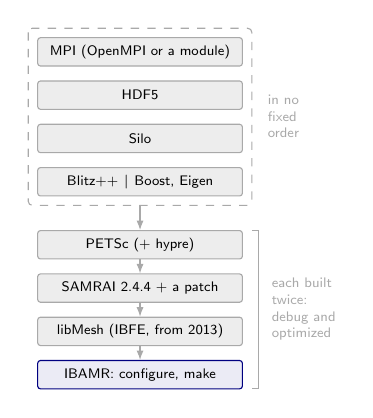
\begin{tikzpicture}[every node/.style={font=\tiny\sffamily}, lib/.style={draw=DarkGray, fill=LightGray!40, rounded corners=1pt, minimum width=2.6cm, minimum height=0.36cm, inner sep=1.5pt}, ar/.style={-{Latex[length=1.2mm]},DarkGray}]
  \node[lib] (mpi) at (0,0) {MPI (OpenMPI or a module)};
  \node[lib] (hdf) at (0,-0.55) {HDF5};
  \node[lib] (silo) at (0,-1.1) {Silo};
  \node[lib] (bl) at (0,-1.65) {Blitz++ \textbar\ Boost, Eigen};
  \draw[DarkGray, dashed, rounded corners=1.5pt] (-1.42,0.3) rectangle (1.42,-1.95);
  \node[font=\tiny\sffamily,text=DarkGray,align=left,anchor=west] at (1.5,-0.82) {in no\\fixed\\order};
  \node[lib] (pet) at (0,-2.45) {PETSc (+ hypre)};
  \node[lib] (sam) at (0,-3.0) {SAMRAI 2.4.4 + a patch};
  \node[lib] (lm) at (0,-3.55) {libMesh (IBFE, from 2013)};
  \node[lib,draw=NavyBlue,fill=NavyBlue!8] (ib) at (0,-4.1) {IBAMR: configure, make};
  \draw[ar] (0,-1.95) -- (pet);
  \foreach \a/\b in {pet/sam,sam/lm,lm/ib} \draw[ar] (\a) -- (\b);
  \draw[DarkGray] (1.42,-2.27) -- (1.5,-2.27) -- (1.5,-4.28) -- (1.42,-4.28);
  \node[font=\tiny\sffamily,text=DarkGray,align=left,anchor=west] at (1.55,-3.27) {each built\\twice:\\debug and\\optimized};
\end{tikzpicture}}
\end{frame}

% 2
\begin{frame}{Why keep these recipes, and what to use instead}
\label{fr:why}
\begin{columns}[T,onlytextwidth]
\begin{column}{0.53\textwidth}
\small
\begin{itemize}\setlength{\itemsep}{0.5pt}
  \item \al{What this is.} From 2011 to 2019 every IBAMR install was built by hand: eight to ten libraries, each configured, compiled and tested, PETSc, SAMRAI, libMesh and IBAMR usually twice. The course and the lab kept a recipe for each machine and year. This chapter keeps all of them, with the commands as written.
  \item \al{Why keep them.} Old papers, theses and course folders name these versions; the recipes say what a result was computed with, and why old code looks the way it does (chapter X3).
  \item \al{Legacy.} Every listing here is marked ``historical, do not run'': many download addresses are dead, the versions (even those still on GitHub) are a decade old, and several commands have slips that this chapter points out.
\end{itemize}
\end{column}
\begin{column}{0.44\textwidth}
\begin{punchbox}
\small To install IBAMR today, use autoibamr (chapter 2): one script builds the whole stack, IBAMR 0.19.0 by default. To build a program, use CMake (chapter 3).
\end{punchbox}
\vspace{1mm}
\footnotesize \al{Who wrote them.} The instructor's course and lab notes (2011--2020); Boyce Griffith's notes and e-mailed advice, summarized here (2013, 2016); Nick Battista's KillDevil notes (2016); Alex Hoover's module-based build (2015); notes whose author is not recorded or not verified (the Miller lab's 2012 ReadMe and its 2012--13 forces notes and deck, the 2014 undergraduate guide, the 2019 Dogwood PDF); and two sets of Mac notes, kept unattributed.
\end{column}
\end{columns}
\sourcecredit{The recipes of this chapter, compared in October 2026; slide \ref{fr:recipes} lists them by date, machine and author.}
\end{frame}

% 3
\begin{frame}{The stack, and what depends on what}
\label{fr:stack}
\begin{columns}[T,onlytextwidth]
\begin{column}{0.4\textwidth}
\centering
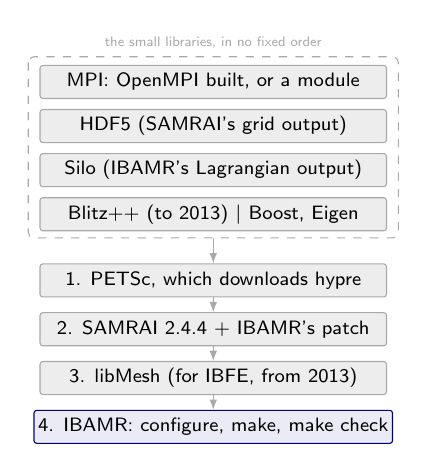
\begin{tikzpicture}[every node/.style={font=\scriptsize\sffamily}, lib/.style={draw=DarkGray, fill=LightGray!40, rounded corners=1pt, minimum width=4.4cm, minimum height=0.42cm, inner sep=1.5pt}, ar/.style={-{Latex[length=1.3mm]},DarkGray}]
  \node[font=\tiny\sffamily,text=DarkGray] at (0,0.5) {the small libraries, in no fixed order};
  \node[lib] (mpi) at (0,0) {MPI: OpenMPI built, or a module};
  \node[lib] (hdf) at (0,-0.56) {HDF5 (SAMRAI's grid output)};
  \node[lib] (silo) at (0,-1.12) {Silo (IBAMR's Lagrangian output)};
  \node[lib] (bl) at (0,-1.68) {Blitz++ (to 2013) \textbar\ Boost, Eigen};
  \draw[DarkGray, dashed, rounded corners=2pt] (-2.35,0.32) rectangle (2.35,-1.98);
  \node[lib] (pet) at (0,-2.52) {1. PETSc, which downloads hypre};
  \node[lib] (sam) at (0,-3.14) {2. SAMRAI 2.4.4 + IBAMR's patch};
  \node[lib] (lm) at (0,-3.76) {3. libMesh (for IBFE, from 2013)};
  \node[lib,draw=NavyBlue,fill=NavyBlue!8] (ib) at (0,-4.38) {4. IBAMR: configure, make, make check};
  \draw[ar] (0,-1.98) -- (pet);
  \foreach \a/\b in {pet/sam,sam/lm,lm/ib} \draw[ar] (\a) -- (\b);
\end{tikzpicture}
\end{column}
\begin{column}{0.57\textwidth}
\scriptsize
\begin{itemize}\setlength{\itemsep}{2pt}
  \item The small libraries were built in no fixed order: the 2012 ReadMe built Blitz++, HDF5 and Silo before OpenMPI, the 2016--19 recipes start with Boost, and the Mavericks notes build Boost and Eigen after SAMRAI.
  \item PETSc, SAMRAI, libMesh (from 2013) and IBAMR always come in that order, each pointed by a path in its \code{configure} line at what it uses: PETSc at MPI; SAMRAI at MPI, HDF5 and Silo; libMesh at PETSc; IBAMR at all of them.
  \item These four are built \al{twice}, a debug build and an optimized build, and the four debug (or optimized) builds must be matched: same paths, same \code{PETSC\_ARCH}.
  \item IBAMR was built with autotools: \code{configure}, then \code{make} (or \code{make lib}) and \code{make check}. A program was compiled with a Makefile that included IBAMR's \code{make.inc} (chapter X3).
  \item autoibamr (chapter 2) builds the same stack today in one command, and IBAMR itself with CMake.
\end{itemize}
\end{column}
\end{columns}
\sourcecredit{All recipes of this chapter; chapter 2.}
\end{frame}

% 4
\begin{frame}{The folder layout every recipe used}
\label{fr:folders}
\small
\begin{columns}[T,onlytextwidth]
\begin{column}{0.55\textwidth}
\scriptsize
\renewcommand{\arraystretch}{1.1}
\setlength{\tabcolsep}{4pt}
\begin{tabular}{@{}L{0.46\linewidth}L{0.5\linewidth}@{}}
\toprule
folder & what goes there \\
\midrule
\code{\$HOME/sfw/linux/\allowbreak <pkg>/<version>} & the small libraries: OpenMPI, HDF5, Silo, Blitz++, later Boost and Eigen \\
\code{\$HOME/sfw/petsc/<version>} & PETSc's source; each \code{PETSC\_ARCH} builds in its own subfolder \\
\code{\$HOME/sfw/samrai/2.4.4/} & \code{SAMRAI} (source), \code{objs-debug} (from 2016 also \code{objs-opt}) (builds), \code{linux-g++-debug}, \code{linux-g++-opt} (installs) \\
\code{\$HOME/sfw/ibamr/} & \code{IBAMR} or \code{IBAMR2} (source), \code{ibamr-objs-debug} or \code{-dbg}, \code{ibamr-objs-opt} (builds) \\
\bottomrule
\end{tabular}
\end{column}
\begin{column}{0.42\textwidth}
\footnotesize
\begin{itemize}\setlength{\itemsep}{2pt}
  \item \al{Variants}: \code{/usr/bin/sfw} (root installs on THLinux, 2013), \code{\$HOME/sfw2} (KillDevil, 2012--13), \code{\$HOME/sfw/killdevil} (2016), \code{\$HOME/Softwares} (the Mavericks notes, about 2015).
  \item A program's Makefile then pointed at the IBAMR source and build folders: \code{IBAMR\_SRC\_DIR} and \code{IBAMR\_BUILD\_DIR} (chapter X3 dates old code by these paths).
  \item \al{The debug build} is for finding errors: assertions on, slow. \al{The optimized build} is for runs.
\end{itemize}
\end{column}
\end{columns}
\sourcecredit{The recipes of 2012--2019; the 2014--2018 course Makefiles.}
\end{frame}

% 5
\begin{frame}{Eight years on one table (1/2): 2012 to 2014}
\label{fr:timeline1}
\tiny
\renewcommand{\arraystretch}{1.15}
\setlength{\tabcolsep}{2.5pt}
\begin{tabular}{@{}L{0.1\textwidth}L{0.12\textwidth}L{0.11\textwidth}L{0.1\textwidth}L{0.05\textwidth}L{0.05\textwidth}L{0.065\textwidth}L{0.08\textwidth}L{0.065\textwidth}L{0.1\textwidth}@{}}
\toprule
when & machine & MPI & Blitz / Boost / Eigen & HDF5 & Silo & PETSc & SAMRAI patch & libMesh & IBAMR \\
\midrule
2012 & lab servers; KillDevil & OpenMPI 1.4.3 (built) & Blitz 0.9 & 1.8.7 & 4.8 & 3.1-p7 & 100922 & -- & SVN \code{trunk} \\
Dec 2012 -- Jan 2013 & lab; KillDevil & as 2012 & Blitz 0.9 & 1.8.7 & 4.8 & 3.2-p6 & 111217 & -- & \code{boyceg} r3262 (forces) \\
April 2013 & lab servers; THLinux & 1.4.3, or PETSc's download & Blitz 0.9 & 1.8.7 & 4.8 & 3.3-p5 & 121212 & 0.8.0 & \code{boyceg} \\
2013 & THLinux (root); KillDevil & 1.4.3 (built) & Blitz 0.9 & 1.8.7 & 4.8 & 3.3-p5 & 121212 & 0.8.0 & \code{boyceg}; \code{ibamr-dev} r3606 \\
Dec 2013 & THLinux; a developer's Mac & 1.4.3; PETSc's & Boost, Eigen (Blitz removed) & 1.8.7 & 4.8 (4.9.1 advised) & 3.3-p5 & 121212 & 0.9.1, 0.9.2 & \code{ibamr-dev} \\
Feb--Mar 2014 & module \code{ibamr/3803} & \code{openmpi\_intel/\allowbreak 11.1} & Boost 1.53.0 & 1.8.5 & 4.9.1 & 3.4 & (module) & 0.9.3 & r3803 \\
\bottomrule
\end{tabular}

\vspace{2mm}
\footnotesize The SAMRAI version never changed: 2.4.4 with a patch from IBAMR's developers, whose date is its name (100922, 111217, 121212). ``--'': no libMesh (IB only). \code{boyceg} and \code{ibamr-dev} are branches of IBAMR's old SVN repository on Google Code.
\sourcecredit{The recipes on the next slides, compared in October 2026.}
\end{frame}

% 6
\begin{frame}{Eight years on one table (2/2): 2015 to today}
\label{fr:timeline2}
\tiny
\renewcommand{\arraystretch}{1.15}
\setlength{\tabcolsep}{2.5pt}
\begin{tabular}{@{}L{0.1\textwidth}L{0.12\textwidth}L{0.11\textwidth}L{0.1\textwidth}L{0.05\textwidth}L{0.05\textwidth}L{0.065\textwidth}L{0.08\textwidth}L{0.065\textwidth}L{0.1\textwidth}@{}}
\toprule
when & machine & MPI & Boost / Eigen & HDF5 & Silo & PETSc & SAMRAI patch & libMesh & IBAMR \\
\midrule
2015 & KillDevil modules & module & Boost 1.53.0 & 1.8.5 & 4.9.1 & 3.4 & (module) & 0.9.3 & GitHub, commit \code{386ab2} \\
about 2015 & Mac OS X 10.9.5 & OpenMPI 1.10.0 & Boost 1.59.0; Eigen 3.2.6 & 1.8.15 & 4.10.2 & 3.5.4 & 121212 & 0.9.4 & master (+ GSL) \\
Apr--Aug 2016 & KillDevil & \code{openmpi\_gcc/\allowbreak 4.8.1} & Boost 1.57.0 & 1.8.16 & 4.10.2 & master & 121212 & master & master \\
Aug 2016 & Mac OS X 10.11.6 & OpenMPI 1.10.2 & Boost 1.61.0 & 1.8.17 & 4.10.2 & 3.7.2 & 121212 & 1.0.0 & master \\
Sep 2016 -- Apr 2017 (module: Nov 2016) & KillDevil; module \code{ibamr/2016-11} & \code{openmpi\_gcc/\allowbreak 4.8.1} & Boost 1.60.0; Eigen 3.2.7 & 1.8.16 & 4.10 & 3.7.2 & 121212 & 1.0.0 & master \\
2018 & Dogwood, module \code{ibamr/2018-03} & \code{openmpi\_2.0.3/\allowbreak gcc\_4.8.5} & \multicolumn{6}{l}{(a module)} & a snapshot from before 0.3.0 \\
2019 & Dogwood & \code{openmpi\_2.0.3/\allowbreak gcc\_4.8.5} & Boost 1.70.0; Eigen 3.3.7 (unused) & 1.10.5 & 4.10.2 & 3.10.5 & \code{ibamr-\allowbreak samrai-\allowbreak fixes} & 1.4.1 & v0.4.1 \\
2020 & Dogwood, module \code{ibamr/0.6.0} & \code{openmpi\_2.0.3/\allowbreak gcc\_4.8.5} & \multicolumn{6}{l}{(a module)} & 0.6.0 \\
2026 & autoibamr (a test install in WSL) & system MPI & Boost 1.91.0; Eigen 3.4.0 (bundled) & 1.12.2 & 4.11 & 3.23.3 & IBSAMRAI2 2025.10.29 & 1.7.8 & 0.19.0 (Puma: 0.16.0) \\
\bottomrule
\end{tabular}

\vspace{2mm}
\footnotesize From 2015 IBAMR came from GitHub (\code{git clone}; in 2019 a release tarball); in 2016 PETSc and libMesh sometimes came from their moving \code{master} branches. The last row is today's install (chapter 2), for comparison.
\sourcecredit{The recipes of this chapter, compared in October 2026; IBAMR's release tags; the packages of a test install of autoibamr in WSL (October 2026).}
\end{frame}

% 7
\begin{frame}{How to read an old recipe (1/3): five invisible copy-and-paste traps}
\label{fr:traps}
\scriptsize
\renewcommand{\arraystretch}{1.15}
\setlength{\tabcolsep}{4pt}
\begin{tabular}{@{}L{0.17\textwidth}L{0.42\textwidth}L{0.36\textwidth}@{}}
\toprule
trap & where (examples) & what happens when you paste it \\
\midrule
an em dash for \code{--} & \code{\emdashmark{}-with-hypre=1} (the 2016 KillDevil notes and ``Laura's Install''); \code{./source/scripts/includes \emdashmark{}link} & the option is not recognized \\
non-breaking spaces as indentation & the 2012 ReadMe (358 of them, on 220 lines), the 2013 forces deck and text notes, the 2016 KillDevil notes (86, one at the start of nearly every continued configure line) & the shell reads \code{\textbackslash xa0./configure} as one unknown word (\code{command not found}), or hands \code{configure} a stray argument (\code{invalid host type}); the 2016 notes' workaround, pasting through an e-mail, turned them into ordinary spaces \\
\bottomrule
\end{tabular}

\vspace{2mm}
\footnotesize In this chapter the traps are shown as they were, the invisible ones marked: an em dash is printed as a red \emdashmark, a curly quote as a red \curlyclose, and \code{\textvisiblespace} marks a space after a continuation backslash (other trailing spaces, harmless, are left out). Non-breaking spaces are shown as ordinary spaces. A modern editor shows them all; a slide or a word processor does not.
\sourcecredit{The recipes of this chapter, checked in their original files (October 2026).}
\end{frame}

% 7b
\begin{frame}{How to read an old recipe (2/3): the traps, continued}
\label{fr:traps2}
\scriptsize
\renewcommand{\arraystretch}{1.15}
\setlength{\tabcolsep}{4pt}
\begin{tabular}{@{}L{0.17\textwidth}L{0.42\textwidth}L{0.36\textwidth}@{}}
\toprule
trap & where (examples) & what happens when you paste it \\
\midrule
a space after the continuation backslash & \code{--with-c++-support \textbackslash\textvisiblespace} (2012 PETSc); \code{CXX=g++-mp-4.9 \textbackslash\textvisiblespace\textvisiblespace} (2016 El Capitan HDF5; a Silo line has three spaces) & the backslash escapes the space instead of the line end: the command stops there, with a stray argument (a lone space), and the lines after it run as separate commands \\
curly quotes & \code{CFLAGS="-g -O1 -Wall\curlyclose{}} (2012 speaker notes); \code{--CXXOPTFLAGS="-O3\curlyopen{}} (2013 forces deck) & an unterminated string: the shell waits for more input \\
soft line breaks & ``Laura's Install'' (2016--17) keeps the lines of most command blocks as soft line breaks, one paragraph per block (163 soft breaks in 33 paragraphs) & readers that drop soft breaks run the commands together \\
\bottomrule
\end{tabular}
\sourcecredit{The recipes of this chapter, checked in their original files (October 2026).}
\end{frame}

% 8
\begin{frame}{How to read an old recipe (3/3): the slips that recur}
\label{fr:slips}
\scriptsize
\renewcommand{\arraystretch}{1.12}
\setlength{\tabcolsep}{4pt}
\begin{tabular}{@{}L{0.2\textwidth}L{0.75\textwidth}@{}}
\toprule
kind & examples \\
\midrule
a label that disagrees with the command & a header says PETSc 3.1-p7, the commands build 3.2-p6 (forces notes, 2012); the text names SAMRAI patch 111217, the command applies 121212 (THLinux, 2013) \\
the wrong folder & the SAMRAI patch run inside \code{SAMRAI} while the \code{.gz} sits one level up; an SVN checkout outside the folder the build expects; \code{mkdir} without \code{cd} \\
a name that changes halfway & \code{ibamr-objs-dbg} made, \code{ibamr-objs-debug} used; \code{sfw} for \code{sfw2}; \code{../IBAMR} for \code{IBAMR2}; Boost 1.60.0 in a folder named \code{1.6.0} \\
placeholders & \code{path/to/...}, \code{/path/to/libmesh-dbg}, \code{openmpi\_\_\_}, \code{wget SAMRAI} \\
a Mac path on Linux & \code{--with-boost=/sw}: Fink's folder on the developer's Mac, copied into Linux recipes \\
root on a cluster & ``Log in as root'' in the KillDevil slides (right only on the lab's own THLinux servers) \\
duplicated options & \code{--download-f-blas-lapack=yes} together with \code{=1} or \code{=ifneeded}; \code{--without-petsc} twice \\
an option renamed & \code{--with-libmesh-compile-mode} kept after December 2013, when it became \code{--with-libmesh-method} \\
dead addresses & Google Code SVN, SourceForge SVN, Bitbucket (PETSc, Eigen), the old LLNL pages for SAMRAI and Silo, sharp-n.org \\
an old example path & \code{examples/IB/staggered\_grid/explicit/ex0} (in the recipes to 2017; IBAMR itself had moved it to \code{examples/IB/explicit/ex0} by v0.1-rc1, May 2014) \\
\bottomrule
\end{tabular}
\sourcecredit{The recipes of this chapter, compared in October 2026.}
\end{frame}

% 9
\begin{frame}[fragile]{2011--13: the machines}
\label{fr:machines}
\begin{columns}[T,onlytextwidth]
\begin{column}{0.5\textwidth}
\footnotesize
\begin{itemize}\setlength{\itemsep}{2pt}
  \item \al{The lab's Ubuntu servers} (two, \code{<host>1} and \code{<host>2}; 2012): packages with \code{sudo apt-get install}, the stack in the home folder.
  \item \al{THLinux}, UNC's ``Tar Heel Linux'' (it used \code{yum}, like Red Hat and Fedora): by September 2013 the same two servers ran it, with one stack built as root in \code{/usr/bin/sfw} for everyone (chapter X1); packages with \code{yum}; it also ran inside VirtualBox.
  \item \al{KillDevil}, UNC's cluster: the stack in the home folder (\code{\$HOME/sfw2}), with the cluster's \code{openmpi\_gcc} module; from 2014, IBAMR modules (slide \ref{fr:m3803}).
\end{itemize}
\end{column}
\begin{column}{0.47\textwidth}
\hist{2012 ReadMe, slide 15: ``Other things to install on a new system'' (one item per line on the slide)}
\begin{lstlisting}[style=hist]
# "Use the command sudo apt-get install [package]"
texinfo  blas  tex  texi2html  libwxbase  m4  openmpi-dev  mpiexec or mpirun
\end{lstlisting}
\hist{THLinux slides, slide 1: ``Things to add to new THLinux'' (one item per line on the slide)}
\begin{lstlisting}[style=hist]
scipy ipython python-matplotlib filezilla texi2html graphviz screen fftw-devel
\end{lstlisting}
\hist{2012 ReadMe, slide 16: KillDevil, ``Before you begin''}
\begin{lstlisting}[style=hist]
export FC=gfortran CC=gcc CXX=g++ F77=gfortran
module add openmpi_gcc; module initadd openmpi_gcc
\end{lstlisting}
\end{column}
\end{columns}
\sourcecredit{The Miller lab's IBAMR ReadMe (2012); the instructor's ``Install THLinux and IBAMR'' slides (about 2011--13); host names replaced by \code{<host>}.}
\end{frame}

% 10
\begin{frame}[fragile]{THLinux housekeeping: \code{yum}, root, Dropbox, VirtualBox}
\label{fr:thlinux}
\begin{columns}[T,onlytextwidth]
\begin{column}{0.48\textwidth}
\footnotesize
``How to install on new system (installed as root)'': ``Instead of `sudo-apt install <package>' use `yum install <package>' \ldots\ `./configure' is now `sh ./configure' \ldots\ Had to be logged as root to `sh ./configure'{}''

\vspace{2mm}
Dropbox on THLinux needed a repository fix written for Fedora 15:
\hist{THLinux slides, slides 3--4}
\begin{lstlisting}[style=hist]
Sudo yum install nautilus-dropbox
gedit /etc/yum.repos.d/dropbox.repo
# comment out
baseurl=http://linux.dropbox.com/fedora/$releasever/
# and add
baseurl=http://linux.dropbox.com/fedora/14/
\end{lstlisting}
\end{column}
\begin{column}{0.49\textwidth}
\footnotesize
THLinux in VirtualBox, to share a Windows folder (December 2013):
\hist{``Notes on THLinux''}
\begin{lstlisting}[style=hist]
1. Devices -> Install Guest Additions
2. sudo mount -t vboxsf MyDocuments /home/<user>/Desktop/MyDocuments
\end{lstlisting}
\begin{itemize}\setlength{\itemsep}{2pt}
  \item Root installs in \code{/usr/bin/sfw} put a software tree inside a folder meant for system programs; on a shared machine a home-folder install is safer.
  \item The Dropbox fix is for a release that no longer exists. Today: WSL or a Linux machine with \code{apt} (chapter 2).
\end{itemize}
\end{column}
\end{columns}
\sourcecredit{The instructor's ``Install THLinux and IBAMR'' slides 2--4; ``Notes on THLinux'' (December 2013; user name replaced).}
\end{frame}

% 11
\begin{frame}[fragile]{New accounts and disk quotas on the lab's THLinux servers}
\label{fr:quotas}
\begin{columns}[T,onlytextwidth]
\begin{column}{0.55\textwidth}
\hist{THLinux slides, slides 23--25: ``Set up stuff for new accounts''}
\begin{lstlisting}[style=hist]
Add users: useradd onyen
# the /home line of /etc/fstab, with usrquota,grpquota added (as root):
/dev/VolGroup00/LogVol02 /home ext3 defaults,usrquota,grpquota 1 2
mount -o remount /home
quotacheck -cugm /home
edquota username
# quota -u <user> # Check quota for a user
# repquota /home # Full report for the partition for all users
Default amounts:
50000000 for grad student
25000000 for ugrad
\end{lstlisting}
\end{column}
\begin{column}{0.42\textwidth}
\scriptsize
\begin{itemize}\setlength{\itemsep}{2pt}
  \item An account per student (named by the student's UNC ``onyen''), and a disk quota on \code{/home} so that one IBAMR install could not fill the disk.
  \item \code{edquota} opens a user's limits in an editor; the slides' defaults were 50000000 for a graduate student and 25000000 for an undergraduate, in \code{edquota}'s 1 KB blocks (about 50 GB and 25 GB).
  \item In \code{\# quota -u <user>} and \code{\# repquota /home} the first \code{\#} is the slide's root prompt, not a comment.
  \item The same slides add two pages of \code{vi} commands (\code{:q}, \code{:x}, \code{i I a A o O}).
  \item Today a cluster account comes from the university (chapter 1); quotas are the cluster's.
\end{itemize}
\end{column}
\end{columns}
\sourcecredit{The instructor's ``Install THLinux and IBAMR'' slides 23--25 (a user name in the \code{quota} example replaced by \code{<user>}).}
\end{frame}

% 12
\begin{frame}[fragile]{Blitz++ 0.9 and its two patches (2012--13)}
\label{fr:blitz}
\begin{columns}[T,onlytextwidth]
\begin{column}{0.5\textwidth}
\hist{2012 ReadMe, slide 17}
\begin{lstlisting}[style=hist]
cd $HOME/sfw/linux
tar xvfz blitz-0.9.tar.gz
 cd blitz-0.9
 ./configure \
   CC=gcc \
   CXX=g++ \
   F77=gfortran \
   FC=gfortran \
   --prefix=$HOME/sfw/linux/blitz/0.9 \
   --enable-optimize \
   --disable-debug \
   --enable-shared
cd blitz
wget http://www.sharp-n.org/patches/mathfunc.h.patch
wget http://www.sharp-n.org/patches/funcs.h.patch
patch funcs.h funcs.h.patch
patch mathfunc.h mathfunc.h.patch
cd ..
 make
 make check-testsuite
 make install
\end{lstlisting}
\end{column}
\begin{column}{0.47\textwidth}
\footnotesize
\begin{itemize}\setlength{\itemsep}{2pt}
  \item Blitz++ gave IBAMR its array classes (\code{TinyVector} for positions) until December 2013, when IBAMR replaced it with Boost and Eigen (slide \ref{fr:dec2013}).
  \item The two patches came from a third-party web site that is gone.
  \item \al{A slip} in the KillDevil and THLinux slides: \code{--prefix=\$HOME/sfw2/linux/\allowbreak blitz-0.9\textbackslash} has no space before the backslash, so the next option is glued onto the prefix, and the folder differs from the one IBAMR is later told to use, \code{--with-blitz=\$HOME/sfw2/linux/\allowbreak blitz/0.9}.
  \item The indentation of the 2012 lines is made of non-breaking spaces, mixed with ordinary ones (slide \ref{fr:traps}).
\end{itemize}
\end{column}
\end{columns}
\sourcecredit{The Miller lab's IBAMR ReadMe (2012), slide 17; the instructor's KillDevil slide 4 and THLinux slide 6.}
\end{frame}

% 13
\begin{frame}[fragile]{HDF5 1.8.7, Silo 4.8 and OpenMPI 1.4.3 (2012--13)}
\label{fr:hdf5}
\begin{columns}[T,onlytextwidth]
\begin{column}{0.32\textwidth}
\hist{2012 ReadMe, slide 18}
\begin{lstlisting}[style=hist]
cd $HOME/sfw/linux
tar xvfz hdf5-1.8.7.tar.gz
 cd hdf5-1.8.7
 ./configure \
   CC=gcc \
   CXX=g++ \
   FC=gfortran \
   F77=gfortran \
   --enable-production \
   --disable-debug \
   --prefix=$HOME/sfw/linux/hdf5/1.8.7
 make
 make check
 make install
\end{lstlisting}
\end{column}
\begin{column}{0.3\textwidth}
\hist{slide 19}
\begin{lstlisting}[style=hist]
cd $HOME/sfw/linux
tar xvfz silo-4.8.tar.gz
 cd silo-4.8
 ./configure \
   CC=gcc \
   CXX=g++ \
   FC=gfortran \
   F77=gfortran \
   --prefix=$HOME/sfw/linux/silo/4.8 \
   --disable-silex
 make
 make install
\end{lstlisting}
\end{column}
\begin{column}{0.35\textwidth}
\hist{slide 20}
\begin{lstlisting}[style=hist]
cd $HOME/sfw/linux
tar xvfj openmpi-1.4.3.tar.bz2
 cd openmpi-1.4.3
 ./configure \
   CC=gcc \
   CXX=g++ \
   FC=gfortran \
   F77=gfortran \
   --prefix=$HOME/sfw/linux/openmpi/1.4.3 \
   --disable-mpi-cxx-seek \
   --disable-heterogeneous \
   --enable-orterun-prefix-by-default
 make
 make check
 make install
\end{lstlisting}
\end{column}
\end{columns}
\vspace{1mm}
\footnotesize The three quiet builds: HDF5 is the format of SAMRAI's VisIt files (the grid data); Silo is the library IBAMR writes its Lagrangian data with, in Silo's own PDB format, and no recipe gives Silo \code{--with-hdf5} (\code{--disable-silex} skips Silo's file browser); OpenMPI gives \code{mpicc}, \code{mpicxx}, \code{mpif90} and \code{mpirun}. The KillDevil and THLinux slides are the same with \code{\$HOME/sfw2} or \code{/usr/bin/sfw}, and \code{sh ./configure} for Silo (both) and OpenMPI (THLinux); their OpenMPI slide is labelled ``opempi-1.4.3''.
\sourcecredit{The Miller lab's IBAMR ReadMe (2012), slides 18--20; the instructor's KillDevil slides 5--7.}
\end{frame}

% 14
\begin{frame}[fragile]{PETSc 3.1-p7 (2012) (1/2): unpack, and the debug build}
\label{fr:petsc31}
\begin{columns}[T,onlytextwidth]
\begin{column}{0.56\textwidth}
\hist{2012 ReadMe, slides 21--22 (\textvisiblespace: a space after the backslash)}
\begin{lstlisting}[style=hist]
 cd $HOME/sfw
 mkdir petsc
 cd petsc
 tar xvfz petsc-3.1-p7.tar.gz
 mv petsc-3.1-p7 3.1-p7
 cd 3.1-p7
# Configure debugging petsc
export PETSC_DIR=$PWD
 export PETSC_ARCH=linux
 ./config/configure.py \
   --CC=$HOME/sfw/linux/openmpi/1.4.3/bin/mpicc \
   --CXX=$HOME/sfw/linux/openmpi/1.4.3/bin/mpicxx \
   --FC=$HOME/sfw/linux/openmpi/1.4.3/bin/mpif90 \
   --LDFLAGS="-L$HOME/sfw/linux/openmpi/1.4.3/lib -Wl,-rpath,$HOME/sfw/linux/openmpi/1.4.3/lib" \
   --with-default-arch=0 \
   --PETSC_ARCH=$PETSC_ARCH \
   --with-debugging=1 \
   --with-c++-support \␣
  --download-f-blas-lapack=yes \
  --download-f-blas-lapack=ifneeded \
   --with-hypre=1 \
   --download-hypre=1
 make
 make test
\end{lstlisting}
\end{column}
\begin{column}{0.41\textwidth}
\scriptsize
\begin{itemize}\setlength{\itemsep}{2pt}
  \item \code{PETSC\_DIR} is the source folder, \code{PETSC\_ARCH} names one build of it: \code{linux} (debug) and \code{linux-opt} (optimized) live side by side in the same source tree.
  \item PETSc is compiled with the OpenMPI just built (\code{--CC}, \code{--CXX}, \code{--FC}), and the \code{-rpath} makes the libraries find it at run time.
  \item \code{--download-hypre=1}: PETSc fetches and builds hypre, the multigrid library IBAMR's solvers use; later recipes keep this.
  \item \code{--download-f-blas-lapack} is given twice, with \code{yes} and with \code{ifneeded}.
  \item \code{make test} runs PETSc's own small examples.
\end{itemize}
\end{column}
\end{columns}
\sourcecredit{The Miller lab's IBAMR ReadMe (2012), slides 21--22.}
\end{frame}

% 15
\begin{frame}[fragile]{PETSc 3.1-p7 (2012) (2/2): the optimized build, and the trap in both}
\label{fr:petsc31b}
\begin{columns}[T,onlytextwidth]
\begin{column}{0.5\textwidth}
\footnotesize The optimized build (slide 23) is the debug configure with four changes:
\hist{2012 ReadMe, slide 23, the lines that differ}
\begin{lstlisting}[style=hist]
 export PETSC_ARCH=linux-opt
   --COPTFLAGS="-O3" \
   --CXXOPTFLAGS="-O3" \
   --FOPTFLAGS="-O3" \
   --with-debugging=0 \
   --with-x=0
\end{lstlisting}
\footnotesize The \code{-O3} lines follow \code{--FC}; \code{--with-x=0} is the last line; the \code{--with-c++-support~\textbackslash\textvisiblespace} line is the same as in the debug build.
\end{column}
\begin{column}{0.47\textwidth}
\begin{homebox}
\scriptsize \al{The trap.} In both slides the line \code{--with-c++-support \textbackslash} ends with a space after the backslash. The backslash then escapes the space (configure gets one extra argument, a lone space) instead of the line end, so the configure command ends there, before the BLAS/LAPACK and hypre options. The lines after it (four in the debug build, five in the optimized), still joined by their own backslashes, run as one separate command and fail: \code{--download-f-blas-lapack=yes: command not found}. Even if PETSc's configure then succeeds, it has no hypre, and IBAMR's \code{--with-hypre} later finds nothing.
\end{homebox}
\vspace{1mm}
\scriptsize The cure, then and now: no character after a continuation backslash. A modern editor shows trailing spaces; today autoibamr writes these lines itself.
\end{column}
\end{columns}
\sourcecredit{The Miller lab's IBAMR ReadMe (2012), slides 22--23.}
\end{frame}

% 16
\begin{frame}[fragile]{SAMRAI 2.4.4 (2012): unpack and patch}
\label{fr:samrai2012}
\begin{columns}[T,onlytextwidth]
\begin{column}{0.47\textwidth}
\hist{2012 ReadMe, slide 24}
\begin{lstlisting}[style=hist]
 cd $HOME/sfw
 mkdir samrai
 cd samrai
 mkdir 2.4.4
 cd 2.4.4
 tar xvfz SAMRAI-v2.4.4.tar.gz
# "Next, patch SAMRAI using the patch file
#  SAMRAI-v2.4.4-patch-100922.gz:"
 cd SAMRAI
 ./source/scripts/includes --link
 gunzip -c ../SAMRAI-v2.4.4-patch-100922.gz | patch -p2
\end{lstlisting}
\hist{slide 25, the build folder}
\begin{lstlisting}[style=hist]
 cd $HOME/sfw/samrai/2.4.4
 mkdir objs-debug
 cd objs-debug
# slide 26 (optimized) has no mkdir or cd:
#   it is configured in objs-debug too
\end{lstlisting}
\end{column}
\begin{column}{0.5\textwidth}
\scriptsize
\begin{itemize}\setlength{\itemsep}{2pt}
  \item SAMRAI is LLNL's adaptive mesh library; IBAMR used version 2.4.4, with patches from IBAMR's developers, throughout these recipes, and still does as their fork IBSAMRAI2, which autoibamr builds.
  \item \code{includes --link} makes SAMRAI's header links; the patch is piped through \code{gunzip} into \code{patch -p2} from inside \code{SAMRAI}, so the \code{.gz} must sit one folder up: \code{../}.
  \item The patch changed with the date: 100922 (2012), 111217 (the forces branch), 121212 (2013--2017, later attached to IBAMR's v0.1-rc1 release on GitHub), \code{ibamr-samrai-fixes.patch} (2019).
  \item SAMRAI is configured in a build folder beside its source, \code{objs-debug} (the optimized build reused it until 2016; from August 2016 it has its own \code{objs-opt}), and installed in another (\code{linux-g++-debug}, \code{linux-g++-opt}): next slides.
\end{itemize}
\end{column}
\end{columns}
\sourcecredit{The Miller lab's IBAMR ReadMe (2012), slides 24--26; the later recipes of this chapter.}
\end{frame}

% 17
\begin{frame}[fragile]{SAMRAI's configure, flag by flag (1/5): the list used 2012--2019}
\label{fr:samraiflags}
\begin{columns}[T,onlytextwidth]
\begin{column}{0.45\textwidth}
\hist{``Laura's Install'' (2016), the debug build}
\begin{lstlisting}[style=hist]
../SAMRAI-2.4.4/configure \
  --prefix=$HOME/sfw/samrai/2.4.4/linux-g++-debug \
  --with-CC=gcc \
  --with-CXX=g++ \
  --with-F77=gfortran \
  --with-MPICC=mpicc \
  --with-hdf5=$HOME/sfw/linux/hdf5/1.8.16 \
  --without-hypre \
  --with-silo=$HOME/sfw/linux/silo/4.10 \
  --without-blaslapack \
  --without-cubes \
  --without-eleven \
  --without-kinsol \
  --without-petsc \
  --without-sundials \
  --without-x \
  --with-doxygen \
  --with-dot \
  --enable-debug \
  --disable-opt \
  --enable-implicit-template-instantiation \
  --disable-deprecated
make
make install
\end{lstlisting}
\end{column}
\begin{column}{0.52\textwidth}
\scriptsize
\begin{itemize}\setlength{\itemsep}{2pt}
  \item Nearly the same option list appears in every recipe of this chapter, from the 2012 ReadMe to the 2019 Dogwood PDF: the paths, the compilers and the versions change (slides \ref{fr:samraivar1}--\ref{fr:samraivar3}), and two recipes change the list itself (the 2016 KillDevil notes leave out \code{--with-silo} and add \code{-g -O0} flags to the debug build; the 2019 PDF lists \code{--without-petsc} twice).
  \item \code{--prefix}: where \code{make install} puts SAMRAI; IBAMR's \code{--with-samrai} points here.
  \item \code{--with-CC}, \code{--with-CXX}, \code{--with-F77}, \code{--with-MPICC}: the compilers. In 2012--13 \code{--with-MPICC} was the home-built OpenMPI's \code{mpicc}; in 2019 the compilers themselves were \code{mpicc}, \code{mpicxx}, \code{mpifort}.
  \item \code{--with-hdf5}, \code{--with-silo}: the two output libraries built before.
\end{itemize}
\end{column}
\end{columns}
\sourcecredit{``Laura's Install'' (2016--17); the other recipes of 2012--2019, compared in October 2026.}
\end{frame}

% 17b
\begin{frame}{SAMRAI's configure, flag by flag (2/5): what is switched off, and the optimized build}
\label{fr:samraiflags2}
\begin{columns}[T,onlytextwidth]
\begin{column}{0.55\textwidth}
\small
\begin{itemize}\setlength{\itemsep}{3pt}
  \item The \code{--without-...} options switch off SAMRAI's own links to solvers (hypre, PETSc, SUNDIALS, KINSOL, BLAS/LAPACK) and optional outside packages (the CUBES and Eleven embedded-boundary libraries, and X11): IBAMR reaches PETSc and hypre itself.
  \item \code{--with-doxygen}, \code{--with-dot}: SAMRAI's documentation tools.
  \item \code{--enable-implicit-template-instantiation} and \code{--disable-deprecated}: as IBAMR's own build instructions asked.
  \item \code{--enable-debug --disable-opt} make the debug build.
\end{itemize}
\end{column}
\begin{column}{0.42\textwidth}
\begin{punchbox}
\small \al{The optimized build} adds \code{CFLAGS="-O3" CXXFLAGS="-O3" FFLAGS="-O3"} before \code{--prefix}, installs into \code{.../linux-g++-opt}, and has \code{--disable-debug --enable-opt} in place of \code{--enable-debug --disable-opt}; the rest of the list is the same.
\end{punchbox}
\vspace{2mm}
\footnotesize Then \code{make} and \code{make install}, in each build folder.
\end{column}
\end{columns}
\sourcecredit{``Laura's Install'' (2016--17); the other recipes of this chapter.}
\end{frame}

% 17c
\begin{frame}{SAMRAI's configure, flag by flag (3/5): how the step varied, 2012--2013}
\label{fr:samraivar1}
\tiny
\renewcommand{\arraystretch}{1.0}
\setlength{\tabcolsep}{3pt}
\begin{tabular}{@{}L{0.13\textwidth}L{0.3\textwidth}L{0.21\textwidth}L{0.19\textwidth}L{0.1\textwidth}@{}}
\toprule
recipe & patch, and how it was applied & installed in (debug, optimized) & MPI compiler & HDF5 / Silo \\
\midrule
2012 ReadMe & 100922: \code{cd SAMRAI; ./source/scripts/includes --link; gunzip -c ../SAMRAI-v2.4.4-patch-100922.gz | patch -p2}; configured from \code{objs-debug}, after \code{export PETSC\_ARCH=linux} (or \code{linux-opt}) & \code{\$HOME/sfw/samrai/2.4.4/\allowbreak linux-g++-\{debug,opt\}} & the home-built OpenMPI 1.4.3's \code{mpicc} & 1.8.7 / 4.8 \\
forces notes (2012--13) & 111217: \code{gunzip -c ../SAMRAI-v2.4.4-patch-111217.gz | patch -p2}; \code{./configure} in the source folder & optimized only: \code{\$HOME/sfw/SAMRAI\_petsc3p2/\allowbreak linux-g++-opt} & as 2012 & 1.8.7 / 4.8 \\
``InstallNotes2'' (2013) & 111217; \code{./configure} in \code{\$HOME/sfw/samrai\_petsc3p2/2.4.4/SAMRAI} & optimized only: \code{\$HOME/sfw/samrai\_petsc3p2/\allowbreak linux-g++-opt} & as 2012 & 1.8.7 / 4.8 \\
KillDevil (2012--13) & 121212: \code{cd SAMRAI; ./source/scripts/includes --link; gunzip -c SAMRAI-v2.4.4-patch-121212.gz | patch -p2}, from the wrong folder (the \code{.gz} is one level up) & \code{\$HOME/sfw2/samrai/2.4.4/\allowbreak linux-g++-\{debug,opt\}} & \code{\$HOME/sfw2/linux/openmpi/\allowbreak 1.4.3/bin/mpicc} & 1.8.7 / 4.8 \\
THLinux (2013) & the text says 111217, the command applies 121212 (the same wrong-folder command) & \code{/usr/bin/sfw/samrai/2.4.4/\allowbreak linux-g++-\{debug,opt\}} & \code{/usr/bin/sfw/linux/\allowbreak openmpi/1.4.3/bin/mpicc} & 1.8.7 / 4.8 \\
``THLinuxInstall'' (April 2013) & names \code{SAMRAI-v2.4.4-patch-121212.gz} only & \code{\$HOME/sfw/samrai/2.4.4/\allowbreak linux-g++-\{debug,opt\}} & PETSc's: \code{\$HOME/sfw/petsc/3.3-p5/\allowbreak linux/bin/mpicc} & 1.8.7 / 4.8 \\
December 2013 notes & 121212, fixed: \code{gunzip -c ../SAMRAI-v2.4.4-patch-121212.gz | patch -p2} & as THLinux & as THLinux & 1.8.7 / 4.8 \\
\bottomrule
\end{tabular}

\tiny The KillDevil, THLinux and December 2013 optimized configures write \code{CXXFLAGS="-O3" FFLAGS="-O3" \textbackslash} on one line (harmless).
\sourcecredit{Each recipe, checked in its original (October 2026).}
\end{frame}

% 17d
\begin{frame}{SAMRAI's configure, flag by flag (4/5): how the step varied, 2015--2016}
\label{fr:samraivar2}
\tiny
\renewcommand{\arraystretch}{1.15}
\setlength{\tabcolsep}{3pt}
\begin{tabular}{@{}L{0.13\textwidth}L{0.33\textwidth}L{0.19\textwidth}L{0.18\textwidth}L{0.1\textwidth}@{}}
\toprule
recipe & patch, and how it was applied & installed in (debug, optimized) & compilers & HDF5 / Silo \\
\midrule
Mavericks notes (about 2015) & 121212 from IBAMR's GitHub release: \code{wget https://github.com/IBAMR/IBAMR/\allowbreak releases/download/v0.1-rc1/\allowbreak SAMRAI-v2.4.4-patch-121212.gz}; \code{gunzip -c \$HOME/Softwares/SAMRAI/2.4.4/\allowbreak SAMRAI-v2.4.4-patch-121212.gz | patch -p2}; \code{../configure} from \code{2.4.4/linux-dbg} & debug only: \code{\$HOME/Softwares/SAMRAI/\allowbreak 2.4.4/linux-dbg} & \code{gcc-mp-4.9}, \code{g++-mp-4.9}, \code{gfortran-mp-4.9}; \code{\$HOME/Softwares/\allowbreak OpenMPI/1.10.0/\allowbreak bin/mpicc} & 1.8.15 / 4.10.2 \\
KillDevil, 2016 (Nick Battista) & 121212, with an extra \code{tar xvfz} of the patch (slide \ref{fr:nb2b}); \code{../SAMRAI/configure} & \code{\$HOME/sfw/samrai/2.4.4/\allowbreak killdevil-gcc-\{opt,dbg\}} & \code{gcc}, \code{g++}, \code{gfortran}; \code{mpicc} & 1.8.16 (in \code{\$HOME/\allowbreak sfw/killdevil}) / none \\
El Capitan (August 2016) & 121212 from the same GitHub release; \code{cd SAMRAI-2.4.4/; ./source/scripts/includes --link; gunzip -c ../SAMRAI-v2.4.4-patch-121212.gz | patch -p2} & \code{\$HOME/sfw/samrai/2.4.4/\allowbreak linux-g++-\{debug,opt\}} & \code{gcc-mp-4.9} \ldots; \code{\$HOME/sfw/linux/\allowbreak openmpi/1.10.2/\allowbreak bin/mpicc} & 1.8.17 / 4.10.2 \\
\bottomrule
\end{tabular}

\vspace{2mm}
\footnotesize The 2016 KillDevil notes build the debug SAMRAI with \code{CFLAGS="-g -O0" CXXFLAGS="-g -O0" FFLAGS="-g -O0"} and leave out \code{--with-silo}.
\sourcecredit{Each recipe, checked in its original (October 2026).}
\end{frame}

% 17e
\begin{frame}{SAMRAI's configure, flag by flag (5/5): how the step varied, 2016--2019}
\label{fr:samraivar3}
\tiny
\renewcommand{\arraystretch}{1.15}
\setlength{\tabcolsep}{3pt}
\begin{tabular}{@{}L{0.13\textwidth}L{0.33\textwidth}L{0.19\textwidth}L{0.18\textwidth}L{0.1\textwidth}@{}}
\toprule
recipe & patch, and how it was applied & installed in (debug, optimized) & compilers & HDF5 / Silo \\
\midrule
``Laura's Install'' (2016--17) & \code{tar xvfz SAMRAI-v2.4.4.tar.gz; mv SAMRAI SAMRAI-2.4.4; cd SAMRAI-2.4.4; ./source/scripts/includes --link;} ``*Put patch in SAMRAI-2.4.4 folder*'' \code{gunzip -c SAMRAI-v2.4.4-patch-121212.gz | patch -p2} & as quoted on slide \ref{fr:samraiflags} & \code{gcc}, \code{g++}, \code{gfortran}; \code{mpicc} & 1.8.16 / 4.10 \\
Dogwood (2019) & a new patch: \code{cp \$HOME/ibamr-samrai-fixes.patch .}; \code{patch -p1 < ibamr-samrai-fixes.patch} & \code{\$HOME/sfw/samrai/2.4.4/\allowbreak linux-g++-\{debug,opt\}} & \code{mpicc}, \code{mpicxx}, \code{mpifort} (no \code{--with-MPICC}) & 1.10.5 / 4.10.2 \\
\bottomrule
\end{tabular}

\vspace{2mm}
\footnotesize The patch changed for the last time in 2019: \code{patch -p1} with a plain patch file, in place of the dated \code{.gz} piped through \code{gunzip}. The 2019 debug line lists \code{--without-petsc} twice and has no backslashes (slide \ref{fr:dw19slips}). Today autoibamr builds IBSAMRAI2, IBAMR's fork of SAMRAI 2.4.4 with the patches applied.
\sourcecredit{Each recipe, checked in its original (October 2026).}
\end{frame}

% 18
\begin{frame}[fragile]{IBAMR from Google Code (2012) (1/3): get it, and the debug build}
\label{fr:ibamr2012}
\begin{columns}[T,onlytextwidth]
\begin{column}{0.48\textwidth}
\hist{2012 ReadMe, slides 27--28}
\begin{lstlisting}[style=hist]
cd $HOME/sfw
 mkdir ibamr
 cd ibamr
 svn co https://ibamr.googlecode.com/svn/trunk IBAMR
# configure and compile a debugging build of IBAMR
 cd $HOME/sfw/ibamr
 mkdir ibamr-objs-debug
 cd ibamr-objs-debug
 export PETSC_ARCH=linux
 export PETSC_DIR=$HOME/sfw/petsc/3.1-p7
 ../IBAMR/configure --config-cache \
   CFLAGS="-g -O1 -Wall" \
   CXXFLAGS="-g -O1 -Wall" \
   FFLAGS="-g -O1 -Wall" \
   FCFLAGS="-g -O1 -Wall" \
\end{lstlisting}
\end{column}
\begin{column}{0.49\textwidth}
\hist{slide 28, continued}
\begin{lstlisting}[style=hist]
   CC=$HOME/sfw/linux/openmpi/1.4.3/bin/mpicc \
   CXX=$HOME/sfw/linux/openmpi/1.4.3/bin/mpicxx \
   F77=$HOME/sfw/linux/openmpi/1.4.3/bin/mpif90 \
   FC=$HOME/sfw/linux/openmpi/1.4.3/bin/mpif90 \
   MPICC=$HOME/sfw/linux/openmpi/1.4.3/bin/mpicc \
   MPICXX=$HOME/sfw/linux/openmpi/1.4.3/bin/mpicxx \
   CPPFLAGS="-DOMPI_SKIP_MPICXX" \
   --with-hypre=$PETSC_DIR/$PETSC_ARCH \
   --with-samrai=$HOME/sfw/samrai/2.4.4/linux-g++-debug \
   --with-hdf5=$HOME/sfw/linux/hdf5/1.8.7 \
   --with-blitz=$HOME/sfw/linux/blitz/0.9 \
   --with-silo=$HOME/sfw/linux/silo/4.8
 make
 make check
\end{lstlisting}
\end{column}
\end{columns}
\sourcecredit{The Miller lab's IBAMR ReadMe (2012), slides 27--28.}
\end{frame}

% 18b
\begin{frame}{IBAMR from Google Code (2012) (2/3): what the configure line says}
\label{fr:ibamr2012x}
\footnotesize
\begin{itemize}\setlength{\itemsep}{3pt}
  \item IBAMR lived in a Subversion repository on Google Code; \code{trunk} was its main line. Google Code closed in January 2016; IBAMR's first GitHub release, v0.1-rc1, is from May 2014.
  \item \code{--config-cache} lets a second configure reuse the first one's answers.
  \item \code{CFLAGS}, \code{CXXFLAGS}, \code{FFLAGS}, \code{FCFLAGS}: \code{-g -O1 -Wall} for the debug build (symbols, light optimization, the common warnings).
  \item \code{CC}, \code{CXX}, \code{F77}, \code{FC}, \code{MPICC}, \code{MPICXX}: the home-built OpenMPI's wrappers, the same ones PETSc was built with.
  \item \code{CPPFLAGS="-DOMPI\_SKIP\_MPICXX"} keeps OpenMPI's C++ bindings out of the build, as most later recipes do.
  \item \code{--with-hypre=\$PETSC\_DIR/\$PETSC\_ARCH}: the hypre that PETSc downloaded into its debug build.
  \item \code{--with-samrai}, \code{--with-hdf5}, \code{--with-blitz}, \code{--with-silo}: the install folders of slides \ref{fr:blitz}--\ref{fr:samraiflags}.
  \item IBAMR was configured in a build folder beside the source (\code{ibamr-objs-debug}), not in the source itself; only the 2016 KillDevil notes configure in the source tree (slide \ref{fr:nb3}).
\end{itemize}
\sourcecredit{The Miller lab's IBAMR ReadMe (2012), slide 28.}
\end{frame}

% 19
\begin{frame}[fragile]{IBAMR from Google Code (2012) (3/3): the optimized build and the first run}
\label{fr:ibamr2012b}
\begin{columns}[T,onlytextwidth]
\begin{column}{0.5\textwidth}
\hist{2012 ReadMe, slide 29: what differs from the debug build}
\begin{lstlisting}[style=hist]
 mkdir ibamr-objs-opt
 cd ibamr-objs-opt
 export PETSC_ARCH=linux-opt
 # CFLAGS, CXXFLAGS, FFLAGS, FCFLAGS = "-O3 -Wall"
   --with-samrai=$HOME/sfw/samrai/2.4.4/linux-g++-opt \
 # then make, make check as before
\end{lstlisting}
\hist{slide 30: ``You may now compile and run the IBAMR examples, e.g.,''}
\begin{lstlisting}[style=hist]
 cd $HOME/sfw/ibamr/ibamr-objs-debug/examples/IB/staggered_grid/explicit/ex0
 make examples
 ./main2d input2d
\end{lstlisting}
\hist{speaker notes of slide 28 (curly closing quotes; shortened)}
\begin{lstlisting}[style=hist]
../IBAMR/configure --config-cache CFLAGS="-g -O1 -Wall” CXXFLAGS="-g -O1 -Wall” FFLAGS="-g -O1 -Wall” FCFLAGS="-g -O1 -Wall” ... CPPFLAGS="-DOMPI_SKIP_MPICXX”
\end{lstlisting}
\end{column}
\begin{column}{0.47\textwidth}
\scriptsize
\begin{itemize}\setlength{\itemsep}{2pt}
  \item In the optimized build the four flag lines come after the \code{MPICXX} line; otherwise it is the debug configure.
  \item \code{make check} adds no tests in IBAMR's autotools build: like \code{make lib} (\code{lib: all}), it builds the libraries. \code{make examples} in an example's build folder compiles that example.
  \item \code{ex0} of \code{IB/staggered\_grid/explicit} was the first example to run; today it is \code{examples/IB/explicit/ex0} in IBAMR's source, and this series starts with its own examples (chapter 3).
  \item The speaker notes held a one-line version of every configure command, handy for pasting except that the closing quotes of slide 28's note are curly (slide \ref{fr:traps}) and a non-breaking space glues its \code{FC=...mpif90} to \code{MPICC=...}.
  \item Running on KillDevil (\code{bsub}, \code{/netscr}) is in chapter X1.
\end{itemize}
\end{column}
\end{columns}
\sourcecredit{The Miller lab's IBAMR ReadMe (2012), slides 28--31 and speaker notes.}
\end{frame}

% 20
\begin{frame}[fragile]{The ``forces'' branch (December 2012 -- January 2013) (1/7): PETSc 3.2-p6}
\label{fr:forces1}
\small A second recipe, of December 2012 -- January 2013, built IBAMR's \code{boyceg} branch at revision 3262, for the lab's work on forces, in optimized form only. It reused Blitz++, HDF5, Silo and OpenMPI from the 2012 recipe and rebuilt PETSc and SAMRAI.

\vspace{1mm}
\hist{``InstallationNotesForces.txt'' (each long command is one line in the file)}
\begin{lstlisting}[style=hist]
**PETSC 3.1-p7*******************************
cd $HOME/sfw/petsc
tar xvfz petsc-3.2-p6.tar.gz
cd petsc-3.2-p6
//CONFIGURE OPTIMIZED PETSC
export PETSC_DIR=$PWD
export PETSC_ARCH=linux-opt
./config/configure.py --CC=$HOME/sfw/linux/openmpi/1.4.3/bin/mpicc --CXX=$HOME/sfw/linux/openmpi/1.4.3/bin/mpicxx --FC=$HOME/sfw/linux/openmpi/1.4.3/bin/mpif90 --COPTFLAGS="-O3" --CXXOPTFLAGS="-O3" --FOPTFLAGS="-O3" --LDFLAGS="-L$HOME/sfw/linux/openmpi/1.4.3/lib -Wl,-rpath,$HOME/sfw/linux/openmpi/1.4.3/lib" --with-default-arch=0 --PETSC_ARCH=$PETSC_ARCH --with-debugging=0 --with-c++-support --download-f-blas-lapack=yes --download-f-blas-lapack=ifneeded --with-hypre=1 --download-hypre=1 --with-x=0
make
make test
\end{lstlisting}
\footnotesize The header says 3.1-p7; every command builds 3.2-p6. The lines starting with \code{//} are notes, not shell comments: pasted into a shell, each gives an error such as \code{//CONFIGURE: No such file or directory}.
\sourcecredit{The Miller lab's forces install notes (text file, December 2012 -- January 2013).}
\end{frame}

% 21
\begin{frame}[fragile]{The ``forces'' branch (2/7): SAMRAI with patch 111217}
\label{fr:forces2}
\hist{``InstallationNotesForces.txt'', continued}
\begin{lstlisting}[style=hist]
**SAMRAI 2.4.4***********************************
 cd $HOME/sfw
 tar xvfz SAMRAI-v2.4.4.tar.gz
mv SAMRAI SAMRAI_petsc3p2
# "Next, patch SAMRAI using the patch file SAMRAI-v2.4.4-patch-111217.gz:"
cd SAMRAI_petsc3p2
./source/scripts/includes --link
gunzip -c ../SAMRAI-v2.4.4-patch-111217.gz | patch -p2
export PETSC_ARCH=linux
//OPTIMIZED SAMRAI
./configure CFLAGS="-O3" CXXFLAGS="-O3" FFLAGS="-O3" --prefix=$HOME/sfw/SAMRAI_petsc3p2/linux-g++-opt --with-CC=gcc --with-CXX=g++ --with-F77=gfortran --with-MPICC=$HOME/sfw/linux/openmpi/1.4.3/bin/mpicc --with-hdf5=$HOME/sfw/linux/hdf5/1.8.7 --without-hypre --with-silo=$HOME/sfw/linux/silo/4.8 --without-blaslapack --without-cubes --without-eleven --without-kinsol --without-petsc --without-sundials --without-x --with-doxygen --with-dot --disable-debug --enable-opt --enable-implicit-template-instantiation --disable-deprecated
make
make install
\end{lstlisting}
\scriptsize
\begin{itemize}\setlength{\itemsep}{2pt}
  \item A separate SAMRAI (\code{SAMRAI\_petsc3p2}) beside the 2012 one, patched with 111217, and configured inside its own source folder.
  \item \code{PETSC\_ARCH=linux} before an optimized SAMRAI: the forces deck adds ``Note: PETSC\_ARCH=linux should perhaps be PETSC\_ARCH=linux-opt''. It does no harm here: SAMRAI is configured \code{--without-petsc}.
  \item A second copy of the file differs only by three stray non-ASCII bytes before the three patch lines.
\end{itemize}
\sourcecredit{The Miller lab's forces install notes (two copies); the forces install deck (January 2013), slide 10.}
\end{frame}

% 22
\begin{frame}[fragile]{The ``forces'' branch (3/7): IBAMR at revision 3262}
\label{fr:forces3}
\hist{``InstallationNotesForces.txt'', continued}
\begin{lstlisting}[style=hist]
**IBAMR FORCES************************
cd $HOME/sfw/
mkdir ibamr_forces
svn co https://ibamr.googlecode.com/svn/branches/boyceg IBAMR
cd IBAMR
svn up -r3262
cd $HOME/sfw/ibamr_forces
mkdir ibamr-objs-opt
cd ibamr-objs-opt
export PETSC_ARCH=linux-opt
export PETSC_DIR=$HOME/sfw/petsc/petsc-3.2-p6
../IBAMR/configure --config-cache CC=$HOME/sfw/linux/openmpi/1.4.3/bin/mpicc CXX=$HOME/sfw/linux/openmpi/1.4.3/bin/mpicxx F77=$HOME/sfw/linux/openmpi/1.4.3/bin/mpif90 FC=$HOME/sfw/linux/openmpi/1.4.3/bin/mpif90 MPICC=$HOME/sfw/linux/openmpi/1.4.3/bin/mpicc MPICXX=$HOME/sfw/linux/openmpi/1.4.3/bin/mpicxx CFLAGS="-O3 -Wall" CXXFLAGS="-O3 -Wall" FFLAGS="-O3 -Wall" FCFLAGS="-O3 -Wall" CPPFLAGS="-DOMPI_SKIP_MPICXX" --with-hypre=$PETSC_DIR/$PETSC_ARCH --with-samrai=$HOME/sfw/SAMRAI_petsc3p2/linux-g++-opt --with-hdf5=$HOME/sfw/linux/hdf5/1.8.7 --with-blitz=$HOME/sfw/linux/blitz/0.9 --with-silo=$HOME/sfw/linux/silo/4.8  --enable-large-ghost-cell-width --enable-expensive-cf-interpolation
make
make check
\end{lstlisting}
\footnotesize The optimized build only, against the SAMRAI of the last slide and the 2012 Blitz++, HDF5 and Silo; then \code{make} and \code{make check}.
\sourcecredit{The Miller lab's forces install notes (December 2012 -- January 2013).}
\end{frame}

% 22b
\begin{frame}{The ``forces'' branch (4/7): what the build adds, and a slip}
\label{fr:forces3b}
\small
\begin{itemize}\setlength{\itemsep}{2pt}
  \item \code{svn up -r3262} pins the branch to one revision. \code{--enable-large-ghost-cell-width} and \code{--enable-expensive-cf-interpolation} are the two options this build adds (by their names: wider ghost-cell regions, and a costlier interpolation at coarse--fine boundaries).
  \item \al{A slip}: \code{mkdir ibamr\_forces} but no \code{cd}: the checkout lands in \code{\$HOME/sfw/IBAMR}, while the build in \code{\$HOME/sfw/ibamr\_forces/ibamr-objs-opt} looks for \code{../IBAMR}. The later text version adds the \code{cd} (slide \ref{fr:forces4c}).
\end{itemize}
\sourcecredit{The Miller lab's forces install notes (December 2012 -- January 2013).}
\end{frame}

% 23
\begin{frame}[fragile]{The ``forces'' branch (5/7): the second text version, PETSc and SAMRAI}
\label{fr:forces4}
\begin{columns}[T,onlytextwidth]
\begin{column}{0.49\textwidth}
\hist{``InstallNotes2.txt'' (2013), PETSc; blank lines left out; ``...'': as in the first file}
\begin{lstlisting}[style=hist]
PETSC3.2-p6
cd $HOME/sfw
mkdir petsc3p2
cd petsc3p2
tar xvfz petsc-3.2-p6.tar.gz
mv petsc-3.2-p6 3.2-p6
cd 3.2-p6
export PETSC_DIR=$PWD
export PETSC_ARCH=linux-opt
./config/configure.py ... --with-c++-support --download-f-blas-lapack=yes --download-f-blas-lapack=1 --with-hypre=1 --download-hypre=1 --with-x=0
make
make test
\end{lstlisting}
\end{column}
\begin{column}{0.48\textwidth}
\hist{SAMRAI}
\begin{lstlisting}[style=hist]
//SAMRAI2.4.4
cd $HOME/sfw
mkdir samrai_petsc3p2
cd samrai_petsc3p2
 mkdir 2.4.4
 cd 2.4.4
 tar xvfz SAMRAI-v2.4.4.tar.gz
# "Next, patch SAMRAI using the patch file SAMRAI-v2.4.4-patch-111217.gz:"
 cd SAMRAI
 ./source/scripts/includes --link
 gunzip -c ../SAMRAI-v2.4.4-patch-111217.gz | patch -p2
cd $HOME/sfw/samrai_petsc3p2/2.4.4/SAMRAI
export PETSC_ARCH=linux
./configure ... --prefix=$HOME/sfw/samrai_petsc3p2/linux-g++-opt ...
make
make install
\end{lstlisting}
\end{column}
\end{columns}
\sourcecredit{The Miller lab's ``InstallNotes2.txt'' (2013).}
\end{frame}

% 29b
\begin{frame}[fragile]{The ``forces'' branch (6/7): the second text version, IBAMR, and what changed}
\label{fr:forces4c}
\begin{columns}[T,onlytextwidth]
\begin{column}{0.53\textwidth}
\hist{``InstallNotes2.txt'' (2013), IBAMR}
\begin{lstlisting}[style=hist]
// IBAMR FORCES
cd $HOME/sfw/
mkdir ibamr_forces
cd ibamr_forces
svn co https://ibamr.googlecode.com/svn/branches/boyceg IBAMR
cd IBAMR
svn up -r3262
cd $HOME/sfw/ibamr_forces
mkdir ibamr-objs-opt
cd ibamr-objs-opt
export PETSC_ARCH=linux-opt
export PETSC_DIR=$HOME/sfw/petsc3p2/3.2-p6
../IBAMR/configure ... --with-samrai=$HOME/sfw/samrai_petsc3p2/linux-g++-opt ...
make
make check
\end{lstlisting}
\end{column}
\begin{column}{0.44\textwidth}
\scriptsize \al{Against the first file}
\begin{itemize}\setlength{\itemsep}{1pt}
  \item the header names the right PETSc, 3.2-p6, unpacked into \code{petsc3p2/3.2-p6};
  \item SAMRAI is unpacked into \code{samrai\_petsc3p2/2.4.4} and keeps the name \code{SAMRAI};
  \item the PETSc line has \code{--download-f-blas-lapack=1} for \code{=ifneeded};
  \item \code{cd ibamr\_forces} is there, so the checkout lands where the build looks for it (slide \ref{fr:forces3b});
  \item the headers are \code{PETSC3.2-p6}, \code{//SAMRAI2.4.4} and \code{// IBAMR FORCES}, in place of three starred headers and two \code{//} notes; pasted, each still gives an error;
  \item six lines begin with a non-breaking space byte, shown here as spaces.
\end{itemize}
\end{column}
\end{columns}
\sourcecredit{The Miller lab's ``InstallNotes2.txt'' (2013) and ``InstallationNotesForces.txt''.}
\end{frame}

% 23b
\begin{frame}{The ``forces'' branch (7/7): the slide deck of January 2013}
\label{fr:forces4b}
\small \al{The forces install deck} (14 slides, January 2013) shows the same steps:
\begin{itemize}\setlength{\itemsep}{2pt}
  \item slide 2: \code{export FC=gfortran CC=gcc CXX=g++ F77=gfortran} and \code{module initadd openmpi\_gcc/4.4.6} on KillDevil;
  \item slides 3--6: Blitz++, HDF5, Silo, OpenMPI as in 2012;
  \item slides 8, 10, 12: the PETSc, SAMRAI and IBAMR configures written over many lines \al{without continuation backslashes}, with \code{--CXXOPTFLAGS="-O3\curlyopen{}} (a curly quote) and \code{--download-f-blas-lapack=yes} with \code{=1}; pasted line by line, every option runs as a command;
  \item slide 13 runs \code{ex0} from \code{ibamr-objs-debug}, which this recipe never builds.
\end{itemize}
The speaker notes hold one-line versions of the configures: those of slides 10 and 12 match the first text file, but the PETSc note (slide 8) has \code{--download-f-blas-lapack=1}, as in ``InstallNotes2.txt'', where the first file has \code{=ifneeded}; slides 3--6 carry one-line notes for Blitz++, HDF5, Silo and OpenMPI, which the text file does not have.
\sourcecredit{The Miller lab's forces install deck (January 2013; author not verified).}
\end{frame}

% 24
\begin{frame}[fragile]{Spring 2013 (1/3): PETSc 3.3-p5 and libMesh 0.8.0, for IBFE}
\label{fr:spring2013}
\begin{columns}[T,onlytextwidth]
\begin{column}{0.55\textwidth}
\hist{MATH 769 ``IBFE install'' slides 2--4 (April 2013)}
\begin{lstlisting}[style=hist]
# "Make clean/make distclean ibamr, samrai, and petsc (or delete them).
#  Install petsc 3.3-p5. Install samrai, updating the petsc version.
#  Now install libmesh version 0.8.0."
# Install a debugging version of libmesh
svn co  https://libmesh.svn.sourceforge.net/svnroot/libmesh/tags/libmesh-0.8.0/libmesh$HOME/sfw//libmesh-dbg
    cd /path/to/libmesh-dbg
    ./configure \
       PETSC_DIR=$HOME/sfw/petsc/3.3-p5 \
       PETSC_ARCH=linux \
       CC=gcc \
       CXX=g++ \
       FC=gfortran \
       F77=gfortran \
       --enable-everything --disable-shared --disable-exceptions
    make METHOD=dbg
# slide 4, optimized: the same into $HOME/sfw//libmesh-opt,
#   with PETSC_ARCH=linux-opt and make METHOD=opt (no cd line)
\end{lstlisting}
\end{column}
\begin{column}{0.42\textwidth}
\scriptsize
\begin{itemize}\setlength{\itemsep}{2pt}
  \item ``You need petsc 3.3-p5 for the most recent version of the Boyce branch.'' IBFE, IBAMR's finite element structures, needed libMesh, so spring 2013 rebuilt the stack around PETSc 3.3-p5 and added libMesh 0.8.0.
  \item libMesh 0.8.0 came from SourceForge's Subversion and was built \al{in its own source folder}: \code{make METHOD=dbg} or \code{METHOD=opt}, no \code{make install}. IBAMR then pointed at that folder.
  \item \al{Slips}: no space between the SVN address and the target folder (\code{.../libmesh\$HOME/\allowbreak sfw//libmesh-dbg}, with a double slash), so \code{svn} gets one argument; \code{/path/to/libmesh-dbg} is a placeholder, and the optimized slide has no \code{cd} at all.
\end{itemize}
\end{column}
\end{columns}
\sourcecredit{The instructor's MATH 769 slides ``IBFE install'' (April 11, 2013), slides 2--4; the host name in the title replaced.}
\end{frame}

% 25
\begin{frame}[fragile]{Spring 2013 (2/3): IBAMR with libMesh}
\label{fr:ibfe2013}
\begin{columns}[T,onlytextwidth]
\begin{column}{0.48\textwidth}
\hist{MATH 769 ``IBFE install'' slides 5--6}
\begin{lstlisting}[style=hist]
 cd $HOME/sfw
 mkdir ibamr
 cd ibamr
svn co https://ibamr.googlecode.com/svn/branches/boyceg IBAMR
 cd $HOME/sfw/ibamr
 mkdir ibamr-objs-debug
 cd ibamr-objs-debug
 export PETSC_ARCH=linux
 export PETSC_DIR=$HOME/sfw/petsc/3.3-p5
 ../IBAMR/configure --config-cache \
   CFLAGS="-g -O1 -Wall" \
   CXXFLAGS="-g -O1 -Wall" \
   FFLAGS="-g -O1 -Wall" \
   FCFLAGS="-g -O1 -Wall" \
\end{lstlisting}
\end{column}
\begin{column}{0.49\textwidth}
\hist{continued}
\begin{lstlisting}[style=hist]
   CC=$HOME/sfw/linux/openmpi/1.4.3/bin/mpicc \
   CXX=$HOME/sfw/linux/openmpi/1.4.3/bin/mpicxx \
   F77=$HOME/sfw/linux/openmpi/1.4.3/bin/mpif90 \
   FC=$HOME/sfw/linux/openmpi/1.4.3/bin/mpif90 \
   MPICC=$HOME/sfw/linux/openmpi/1.4.3/bin/mpicc \
   MPICXX=$HOME/sfw/linux/openmpi/1.4.3/bin/mpicxx \
   CPPFLAGS="-DOMPI_SKIP_MPICXX" \
   --with-hypre=$PETSC_DIR/$PETSC_ARCH \
   --with-samrai=$HOME/sfw/samrai/2.4.4/linux-g++-debug \
   --with-hdf5=$HOME/sfw/linux/hdf5/1.8.7 \
   --with-blitz=$HOME/sfw/linux/blitz/0.9 \
   --with-silo=$HOME/sfw/linux/silo/4.8 \
     --enable-libmesh \
     --with-libmesh=$HOME/sfw/libmesh-dbg \
     --with-libmesh-compile-mode=dbg
 make lib
 make check
\end{lstlisting}
\end{column}
\end{columns}
\sourcecredit{The instructor's MATH 769 slides ``IBFE install'' (April 11, 2013), slides 5--6.}
\end{frame}

% 25b
\begin{frame}{Spring 2013 (3/3): what the libMesh options do, the optimized build, and HDF5}
\label{fr:ibfe2013b}
\small
\begin{itemize}\setlength{\itemsep}{2pt}
  \item The 2012 configure plus three options: \code{--enable-libmesh}, \code{--with-libmesh} (the libMesh source folder) and \code{--with-libmesh-compile-mode=dbg} (which of libMesh's builds to use). \code{make lib} builds the libraries only.
  \item \al{Optimized} (slide 7): \code{ibamr-objs-opt}, \code{PETSC\_ARCH=linux-opt}, \code{"-O3 -Wall"}, \code{linux-g++-opt}, \code{--with-libmesh=\$HOME/\allowbreak sfw/libmesh-opt}, \code{--with-libmesh-compile-mode=opt}; then \code{make} and \code{make check}.
  \item \al{Slide 8}, HDF5 on the lab servers: ``NEW TO \code{<host>}1/2: *Need to use \code{CFLAGS=-O1 ./configure \textbackslash} to get it to work on a newer compiler on ubuntu!''
  \item The debug PETSc build is still called \code{linux}.
\end{itemize}
\sourcecredit{The instructor's MATH 769 slides ``IBFE install'' (April 11, 2013), slides 5--8. Slides 9--13 (FE output in VisIt; the mesh formats libMesh reads) belong to chapters 28 and 17--18.}
\end{frame}

% 26
\begin{frame}[fragile]{Letting PETSc build OpenMPI (THLinux, April 2013)}
\label{fr:petscmpi}
\begin{columns}[T,onlytextwidth]
\begin{column}{0.35\textwidth}
\hist{``THLinuxInstall'' (MATH 769), debug}
\begin{lstlisting}[style=hist]
PETSC debug and opt (with mpi)
export PETSC_DIR=$PWD
export PETSC_ARCH=linux
./config/configure.py \
CC=gcc \
CXX=g++ \
FC=gfortran \
F77=gfortran \
--download-openmpi=1 \
--with-openmpi=1 \
--disable-mpi-cxx-seek \
--disable-heterogeneous \
--enable-orterun-prefix-by-default \
--with-default-arch=0 \
--PETSC_ARCH=$PETSC_ARCH \
--with-debugging=1 \
--with-c++-support \
--with-hypre=1 \
--download-hypre=1
\end{lstlisting}
\end{column}
\begin{column}{0.3\textwidth}
\hist{optimized}
\begin{lstlisting}[style=hist]
export PETSC_DIR=$PWD
export PETSC_ARCH=linux-opt
./config/configure.py \
--CC=gcc \
--CXX=g++ \
--FC=gfortran \
--F77=gfortran \
--COPTFLAGS="-O3" \
--CXXOPTFLAGS="-O3" \
--FOPTFLAGS="-O3" \
--download-openmpi \
--with-openmpi=1 \
--disable-mpi-cxx-seek \
--disable-heterogeneous \
--enable-orterun-prefix-by-default \
--with-default-arch=0 \
--PETSC_ARCH=$PETSC_ARCH \
--with-debugging=0 \
--with-c++-support \
--download-f-blas-lapack=yes \
--download-f-blas-lapack=1 \
--with-hypre=1 \
--download-hypre=1 \
--with-x=0
\end{lstlisting}
\end{column}
\begin{column}{0.32\textwidth}
\scriptsize
\begin{itemize}\setlength{\itemsep}{0.5pt}
  \item \code{--download-openmpi}: PETSc builds its own OpenMPI, and SAMRAI then uses PETSc's \code{mpicc}: \code{--with-MPICC=\$HOME/sfw/\allowbreak petsc/3.3-p5/linux/\allowbreak bin/mpicc}.
  \item SAMRAI with patch 121212; libMesh 0.8.0 as on slide \ref{fr:spring2013} (with a space before the target folder, and a real \code{cd} for the debug build).
  \item \al{Slips}: the debug line gives the compilers as \code{CC=gcc} (no \code{--}), the optimized one as \code{--CC=gcc}; three of OpenMPI's own configure options are handed to PETSc's configure; no \code{make} or \code{make test} for PETSc; the optimized libMesh is configured without \code{cd \$HOME/sfw/\allowbreak libmesh-opt}.
\end{itemize}
\end{column}
\end{columns}
\sourcecredit{The instructor's MATH 769 course folder, ``THLinuxInstall'' (modified April 30, 2013).}
\end{frame}

% 27
\begin{frame}[fragile]{KillDevil home install (2012--13) (1/5): shell, module, disk}
\label{fr:kd1}
\begin{columns}[T,onlytextwidth]
\begin{column}{0.5\textwidth}
\hist{slide 1: ``(1) add these lines to .bash\_profile''}
\begin{lstlisting}[style=hist]
export FC=gfortran CC=gcc CXX=g++ F77=gfortran
# It looks like:
if [ -f /etc/profile.modules ]
then
        . /etc/profile.modules
        export FC=gfortran
        export CC=gcc
        export CXX=g++
        export F77=gfortran
fi
# (2) in the terminal type:
module initadd openmpi_gcc/4.4.6
\end{lstlisting}
\hist{slide 3: ``IBAMR install''}
\begin{lstlisting}[style=hist]
Log in as root
cd $HOME
mkdir sfw2
cd sfw2
Move all installation files here
mkdir linux
cd linux
\end{lstlisting}
\end{column}
\begin{column}{0.47\textwidth}
\scriptsize
\begin{itemize}\setlength{\itemsep}{2pt}
  \item The compilers are set once in \code{.bash\_profile}, inside the block that loads the cluster's modules; \code{module initadd} makes the GNU OpenMPI module load at every login.
  \item Slide 2, disk space: ``Warning! For a second install with libmesh you will not have sufficient space. You can either submit a ticket for more space on killdevil, or delete your old install''.
  \item ``Log in as root'' is copied from the THLinux slides: on a cluster you have no root, and the install goes into \code{\$HOME/sfw2} anyway.
  \item Then Blitz++, HDF5, Silo and OpenMPI 1.4.3 as in 2012 (slides \ref{fr:blitz}--\ref{fr:hdf5}), in \code{\$HOME/sfw2/linux}.
\end{itemize}
\end{column}
\end{columns}
\sourcecredit{The instructor's ``Install IBAMR on KillDevil'' slides 1--7 (about 2012--13).}
\end{frame}

% 28
\begin{frame}[fragile]{KillDevil home install (2/5): PETSc 3.3-p5}
\label{fr:kd2}
\begin{columns}[T,onlytextwidth]
\begin{column}{0.56\textwidth}
\hist{slides 8--9}
\begin{lstlisting}[style=hist]
cd $HOME/sfw2
mkdir petsc
cd petsc
tar xvfz petsc-3.3-p5.tar.gz
cd petsc-3.3-p5
export PATH=$HOME/sfw2/linux/openmpi/1.4.3/bin:$PATH
export MANPATH=$HOME/sfw2/linux/openmpi/1.4.3/share/man:$MANPATH
export LD_LIBRARY_PATH="$HOME/sfw2/linux/openmpi/1.4.3/lib"
# debug
export PETSC_DIR=$PWD
export PETSC_ARCH=linux
./config/configure.py \
--CC=$HOME/sfw2/linux/openmpi/1.4.3/bin/mpicc \
--CXX=$HOME/sfw2/linux/openmpi/1.4.3/bin/mpicxx \
--FC=$HOME/sfw2/linux/openmpi/1.4.3/bin/mpif90 \
--LDFLAGS="-L$HOME/sfw2/linux/openmpi/1.4.3/lib -Wl,-rpath,$HOME/sfw2/linux/openmpi/1.4.3/lib" \
--with-default-arch=0 \
--PETSC_ARCH=$PETSC_ARCH \
--with-debugging=1 \
--with-c++-support \
--with-hypre=1 \
--download-hypre=1
make
make test
\end{lstlisting}
\end{column}
\begin{column}{0.41\textwidth}
\scriptsize
\begin{itemize}\setlength{\itemsep}{2pt}
  \item The home-built OpenMPI is put first on \code{PATH} and \code{MANPATH}, and \code{LD\_LIBRARY\_PATH} is set to its \code{lib} folder, before PETSc is configured.
  \item The slide's own note: ``I used to add this line at the beginning \code{export LD\_LIBRARY\_PATH=\$HOME/sfw2/\allowbreak linux/openmpi/1.4.3/lib} I got a gcc error since it removed gcc-4.4.3 from my library path.'' Setting the variable to one folder drops everything the modules had put there, yet slide 8 itself still does so (with quotes); prepending (\code{...:\allowbreak\$LD\_LIBRARY\_PATH}) keeps the modules' entries.
  \item \al{Optimized} (slide 10): \code{PETSC\_ARCH=linux-opt}; adds \code{--COPTFLAGS="-O3"} \code{--CXXOPTFLAGS="-O3"} \code{--FOPTFLAGS="-O3"}, \code{--with-debugging=0}, \code{--download-f-blas-lapack=yes}, \code{--download-f-blas-lapack=1}, \code{--with-x=0}; \code{make}, \code{make test}.
\end{itemize}
\end{column}
\end{columns}
\sourcecredit{The instructor's ``Install IBAMR on KillDevil'' slides 8--10.}
\end{frame}

% 29
\begin{frame}[fragile]{KillDevil home install (3/5): SAMRAI and libMesh 0.8.0}
\label{fr:kd3}
\begin{columns}[T,onlytextwidth]
\begin{column}{0.5\textwidth}
\hist{slide 11}
\begin{lstlisting}[style=hist]
cd $HOME/sfw2
mkdir samrai
cd samrai
mkdir 2.4.4
cd 2.4.4
tar xvfz SAMRAI-v2.4.4.tar.gz
cd SAMRAI
./source/scripts/includes --link
gunzip -c SAMRAI-v2.4.4-patch-121212.gz | patch -p2
\end{lstlisting}
\footnotesize Slides 12--13: SAMRAI's debug and optimized configures (slide \ref{fr:samraiflags}), after \code{export PETSC\_ARCH=linux} or \code{linux-opt}.

\vspace{1mm}
\al{A slip}: the patch command runs inside \code{SAMRAI}, but the \code{.gz} sits one folder up, beside the SAMRAI tarball; it needs \code{../SAMRAI-v2.4.4-\allowbreak patch-121212.gz}, as in 2012.
\end{column}
\begin{column}{0.47\textwidth}
\hist{slide 14 (15: the same for \code{libmesh-opt}, \code{linux-opt}, \code{METHOD=opt})}
\begin{lstlisting}[style=hist]
svn co  https://libmesh.svn.sourceforge.net/svnroot/libmesh/tags/libmesh-0.8.0/libmesh $HOME/sfw2/libmesh/libmesh-dbg
cd $HOME/sfw2/libmesh/libmesh-dbg
./configure \
PETSC_DIR=$HOME/sfw2/petsc/petsc-3.3-p5 \
PETSC_ARCH=linux \
CC=gcc \
CXX=g++ \
FC=gfortran \
F77=gfortran \
--enable-everything --disable-shared --disable-tbb --disable-cppthreads --disable-exceptions
make METHOD=dbg
http://www.mail-archive.com/libmesh-devel@lists.sourceforge.net/msg04710.html
\end{lstlisting}
\footnotesize Two options more than in April 2013, \code{--disable-tbb} and \code{--disable-cppthreads}, followed on the slide by a link to a message on the libMesh developers' mailing list.
\end{column}
\end{columns}
\sourcecredit{The instructor's ``Install IBAMR on KillDevil'' slides 11--15.}
\end{frame}

% 30
\begin{frame}[fragile]{KillDevil home install (4/5): IBAMR \code{ibamr-dev} at revision 3606}
\label{fr:kd4}
\begin{columns}[T,onlytextwidth]
\begin{column}{0.48\textwidth}
\hist{slides 16--17}
\begin{lstlisting}[style=hist]
cd $HOME/sfw2
mkdir ibamr
cd ibamr
svn co https://ibamr.googlecode.com/svn/branches/ibamr-dev IBAMR2
# "The instructions in this powerpoint only work for an older
#  version of IBAMR. So now you want to go to an older revision:"
cd IBAMR2
svn up -r3606
cd $HOME/sfw2/ibamr
mkdir ibamr-objs-debug
cd ibamr-objs-debug
export PETSC_ARCH=linux
export PETSC_DIR=$HOME/sfw2/petsc/petsc-3.3-p5
../IBAMR2/configure --config-cache \
CFLAGS="-g -O1 -Wall" \
CXXFLAGS="-g -O1 -Wall" \
FFLAGS="-g -O1 -Wall" \
FCFLAGS="-g -O1 -Wall" \
\end{lstlisting}
\end{column}
\begin{column}{0.49\textwidth}
\hist{continued}
\begin{lstlisting}[style=hist]
CC=$HOME/sfw2/linux/openmpi/1.4.3/bin/mpicc \
CXX=$HOME/sfw2/linux/openmpi/1.4.3/bin/mpicxx \
F77=$HOME/sfw2/linux/openmpi/1.4.3/bin/mpif90 \
FC=$HOME/sfw2/linux/openmpi/1.4.3/bin/mpif90 \
MPICC=$HOME/sfw2/linux/openmpi/1.4.3/bin/mpicc \
MPICXX=$HOME/sfw2/linux/openmpi/1.4.3/bin/mpicxx \
CPPFLAGS="-DOMPI_SKIP_MPICXX" \
--with-hypre=$PETSC_DIR/$PETSC_ARCH \
--with-samrai=$HOME/sfw2/samrai/2.4.4/linux-g++-debug \
--with-hdf5=$HOME/sfw2/linux/hdf5/1.8.7 \
--with-blitz=$HOME/sfw2/linux/blitz/0.9 \
--with-silo=$HOME/sfw2/linux/silo/4.8 \
--enable-libmesh \
--with-libmesh=$HOME/sfw2/libmesh/libmesh-dbg \
--with-libmesh-compile-mode=dbg
make lib
make check
\end{lstlisting}
\end{column}
\end{columns}
\sourcecredit{The instructor's ``Install IBAMR on KillDevil'' slides 16--17.}
\end{frame}

% 30b
\begin{frame}[fragile]{KillDevil home install (5/5): the optimized build and the first run}
\label{fr:kd5}
\begin{columns}[T,onlytextwidth]
\begin{column}{0.5\textwidth}
\small
\begin{itemize}\setlength{\itemsep}{2pt}
  \item The \code{ibamr-dev} branch, pinned to revision 3606 because the slides were written for it; the source folder is \code{IBAMR2}.
  \item \al{Optimized} (slide 18): \code{ibamr-objs-opt}, \code{linux-opt}, \code{"-O3 -Wall"}, \code{linux-g++-opt}, \code{libmesh-opt}, \code{--with-libmesh-compile-mode=opt}; \code{make}, \code{make check}.
  \item \al{Run} (slide 19), with a slip: \code{cd \$HOME/sfw/ibamr/ibamr-objs-debug/...} names \code{sfw}, not \code{sfw2}.
\end{itemize}
\end{column}
\begin{column}{0.47\textwidth}
\hist{slide 19}
\begin{lstlisting}[style=hist]
 cd $HOME/sfw/ibamr/ibamr-objs-debug/examples/IB/staggered_grid/explicit/ex0
 make examples
 ./main2d input2d
\end{lstlisting}
\end{column}
\end{columns}
\sourcecredit{The instructor's ``Install IBAMR on KillDevil'' slides 18--19.}
\end{frame}

% 31
\begin{frame}[fragile]{KillDevil: ``Working directions for newer IBAMR -{}- In progress''}
\label{fr:kdnewer}
\begin{columns}[T,onlytextwidth]
\begin{column}{0.5\textwidth}
\hist{``Install IBAMR on KillDevil'', slide 20}
\begin{lstlisting}[style=hist]
cd $HOME/sfw2/ibamr
mkdir ibamr-objs-debug2
cd ibamr-objs-debug2
export LD_LIBRARY_PATH=$HOME/sfw2/linux/openmpi/1.4.3/lib
export PETSC_ARCH=linux
export PETSC_DIR=$HOME/sfw2/petsc/petsc-3.3-p5
sh ../IBAMR/configure --config-cache \
# (here: the debug flags and MPI wrappers of slide 17)
--with-boost=/sw \
--with-hypre=$PETSC_DIR/$PETSC_ARCH \
--with-samrai=$HOME/sfw2/samrai/2.4.4/linux-g++-debug \
--with-hdf5=$HOME/sfw2/linux/hdf5/1.8.7 \
--with-silo=$HOME/sfw2/linux/silo/4.8 \

make
make check
\end{lstlisting}
\end{column}
\begin{column}{0.47\textwidth}
\scriptsize An unfinished attempt at the post-December-2013 IBAMR (no Blitz++, Boost instead). Its problems:
\begin{itemize}\setlength{\itemsep}{2pt}
  \item \code{--with-boost=/sw} is the Fink folder of the developer's Mac (slide \ref{fr:mac2013}); on KillDevil there is no \code{/sw};
  \item it configures \code{../IBAMR}, but the checkout is \code{IBAMR2};
  \item it leaves out libMesh;
  \item its last option ends with a backslash, made harmless by the empty line after it (without that line, \code{make} would become an argument of configure);
  \item \code{export LD\_LIBRARY\_PATH=...} replaces the whole variable, the gcc problem of slide \ref{fr:kd2}.
\end{itemize}
Slides 21--22 (running on KillDevil, changing spring parameters) belong to chapters X1 and X3.
\end{column}
\end{columns}
\sourcecredit{The instructor's ``Install IBAMR on KillDevil'' slide 20.}
\end{frame}

% 32
\begin{frame}{THLinux, as root (2013) (1/2): what differs from KillDevil}
\label{fr:throot}
\small The THLinux slides repeat the KillDevil recipe with these differences:
\begin{itemize}\setlength{\itemsep}{2pt}
  \item ``IBAMR install / Log in as root / cd /usr/bin / mkdir sfw / cd sfw / Move all installation files here / mkdir linux / cd linux'': the stack in \code{/usr/bin/sfw};
  \item \code{sh ./configure} for Blitz++, Silo, OpenMPI and libMesh; the Blitz prefix \code{/usr/bin/sfw/linux/blitz-0.9\textbackslash} (no space);
  \item the PETSc debug slide starts with \code{export LD\_LIBRARY\_PATH=/usr/bin/sfw/\allowbreak linux/openmpi/1.4.3/lib};
  \item libMesh 0.8.0 checked out to \code{/usr/bin/sfw/libmesh/\allowbreak libmesh-dbg}, then \code{cd libmesh-dbg} (relative) and \code{sh ./configure PETSC\_DIR=/usr/bin/sfw/\allowbreak petsc/petsc-3.3-p5 ...};
  \item IBAMR from \code{branches/boyceg} (no revision pin) into \code{IBAMR2}; \code{sh ../IBAMR2/configure --config-cache};
  \item the text names patch 111217, the command applies 121212, from the wrong folder (slide \ref{fr:kd3}).
\end{itemize}
\sourcecredit{The instructor's ``Install THLinux and IBAMR'' slides 5--20 (2013; the deck's Dropbox note dates from about 2011).}
\end{frame}

% 32b
\begin{frame}[fragile]{THLinux, as root (2/2): the \code{LD\_LIBRARY\_PATH} ritual, and Makefile paths}
\label{fr:throot2}
\begin{columns}[T,onlytextwidth]
\begin{column}{0.5\textwidth}
\hist{THLinux slide 21 = ``Running IBAMR on THLinux'' slide 2}
\begin{lstlisting}[style=hist]
Add #include <ibtk/LDataManager.h>  to main.C
IBAMR_SRC_DIR = /usr/bin/sfw/ibamr/IBAMR2
IBAMR_BUILD_DIR = /usr/bin/sfw/ibamr/ibamr-objs-opt
# "You must type this in your terminal every time
#  you run main2d/3d:"
export LD_LIBRARY_PATH=/usr/bin/sfw/linux/openmpi/1.4.3/lib
# "Adding this to .bash_profile and .bashrc does not
#  seem to fix it."
\end{lstlisting}
\vspace{1mm}
\footnotesize The include was the fix for one compile error of that IBAMR (chapter X3); the \code{export} had to be typed at every login because the home-built OpenMPI's libraries were not on the system's library path.
\end{column}
\begin{column}{0.47\textwidth}
\hist{``Running IBAMR on KillDevil'', slide 2}
\begin{lstlisting}[style=hist]
IBAMR_SRC_DIR = $HOME/sfw2/ibamr/IBAMR2
IBAMR_BUILD_DIR = $HOME/sfw2/ibamr/ibamr-objs-opt
# "Warning - Something changed on killdevil so my home directory
#  was messed up, and I had to put in the full path."
IBAMR_SRC_DIR = /pathto/sfw2/ibamr/IBAMR2
IBAMR_BUILD_DIR = /pathto/sfw2/ibamr/ibamr-objs-opt
\end{lstlisting}
\vspace{1mm}
\footnotesize The same Makefile lines on KillDevil, first with \code{\$HOME}, then with the full path. In a Makefile \code{\$HOME} reads as \code{\$H} followed by \code{OME}: \code{\$H} is empty, so the path became \code{OME/sfw2/...}. \code{\$(HOME)} would have worked, then as now (chapter X1).
\end{column}
\end{columns}
\sourcecredit{The instructor's ``Install THLinux and IBAMR'' slide 21, ``Running IBAMR on THLinux'' and ``Running IBAMR on KillDevil'' slides (2013--15; the home path is shown as \code{/pathto}). Running, screen and etiquette: chapter X1.}
\end{frame}

% 33
\begin{frame}{December 2013 (1/2): Blitz++ out, Boost and Eigen in}
\label{fr:dec2013}
\begin{columns}[T,onlytextwidth]
\begin{column}{0.56\textwidth}
\footnotesize Boyce Griffith's advice for the December 2013 rebuild (e-mailed, kept in the instructor's working notes; summarized):
\begin{itemize}\setlength{\itemsep}{2pt}
  \item third-party libraries for the current code: PETSc 3.3, HDF5 1.8.x, a recent Silo (he used 4.9.1), SAMRAI 2.4.4 with the patches from IBAMR's web site;
  \item just committed to \code{branches/ibamr-dev}: \al{Blitz++ removed}. Boost's MultiArray replaces Blitz's Array class and Boost's Array replaces \code{TinyVector} (bundled in \code{ibtk/contrib/boost}, or \code{--with-boost=PATH});
  \item new NDIM-dimensional \code{Matrix}, \code{Vector} and \code{Point} classes based on Eigen (Vector and Point interchangeable, Point by convention for positions; bundled in \code{ibtk/contrib/eigen}, or \code{--with-eigen=PATH});
\end{itemize}
\end{column}
\begin{column}{0.41\textwidth}
\begin{punchbox}
\footnotesize This is the line between the two eras of course code: before it, \code{TinyVector<double,NDIM>} positions; after it, \code{Point} (chapter X3, slide ``Target points: four types for one position'').
\end{punchbox}
\end{column}
\end{columns}
\sourcecredit{The instructor's ``December 2013 IBAMR install working notes'', slides 2--4 (Boyce Griffith's e-mailed notes, summarized).}
\end{frame}

% 33b
\begin{frame}{December 2013 (2/2): muParser, an installed libMesh, and what configure reads from PETSc}
\label{fr:dec2013b}
\small
\begin{itemize}\setlength{\itemsep}{4pt}
  \item muParser moved to \code{ibtk/contrib/muparser} and updated to 2.2.3 (or \code{--with-muparser=PATH});
  \item libMesh 0.9.1 supported, which needs an \al{installed} libMesh (configure, make, make install), pointed at with \code{--with-libmesh=DIR}; and \code{--with-libmesh-compile-mode=METHOD} renamed \code{--with-libmesh-method=METHOD};
  \item with libMesh, Boost must be installed (unpacked is enough: header-only) and the same Boost given to libMesh and IBAMR;
  \item configure now reads the hypre, HDF5, BLAS and LAPACK information from PETSc.
\end{itemize}
\vspace{2mm}
\footnotesize The same notes (slides 5--22) then show a configure line from the developer's Mac and the instructor's THLinux rebuild: the next four slides.
\sourcecredit{The instructor's ``December 2013 IBAMR install working notes'', slides 2--4 (Boyce Griffith's e-mailed notes, summarized).}
\end{frame}

% 34
\begin{frame}[fragile]{A configure line from the developer's Mac (December 2013) (1/2)}
\label{fr:mac2013}
\begin{columns}[T,onlytextwidth]
\begin{column}{0.53\textwidth}
\hist{working notes, slide 5 (the prompt scrubbed)}
\begin{lstlisting}[style=hist]
<host>:ibamr-objs-dbg <user>$ cat configure_command
export PETSC_ARCH=darwin
export PETSC_DIR=$HOME/sfw/petsc/3.3-p5
../IBAMR-dev/configure --config-cache \
 CFLAGS="-g -W -Wall -Wextra" \
 CXXFLAGS="-g -W -Wall -Wextra" \
 FCFLAGS="-g -W -Wall -Wextra" \
 CC=$PETSC_DIR/$PETSC_ARCH/bin/mpicc \
 CXX=$PETSC_DIR/$PETSC_ARCH/bin/mpicxx \
 FC=gfortran \
 MPICC=$PETSC_DIR/$PETSC_ARCH/bin/mpicc \
 MPICXX=$PETSC_DIR/$PETSC_ARCH/bin/mpicxx \
 --with-boost=/sw \
 --with-hdf5=/sw \
 --with-samrai=$HOME/sfw/samrai/2.4.4/darwin-g++-dbg \
 --with-silo=$HOME/sfw/darwin/silo/4.8 \
 --enable-libmesh \
 --with-libmesh=$HOME/sfw/darwin/libmesh/0.9.1-dbg \
 --with-libmesh-method=dbg
\end{lstlisting}
\end{column}
\begin{column}{0.44\textwidth}
\small
\code{/sw} is Fink's folder on a Mac: Boost and HDF5 from the package manager. The compilers are the MPI wrappers PETSc built (\code{\$PETSC\_DIR/\$PETSC\_ARCH/bin/mpicc}), and the new option name \code{--with-libmesh-method} is used.
\end{column}
\end{columns}
\sourcecredit{The instructor's December 2013 working notes, slide 5 (Boyce Griffith's example; machine and user name replaced).}
\end{frame}

% 34b
\begin{frame}{A configure line from the developer's Mac (2/2): the debug and optimized variants}
\label{fr:mac2013b}
\small
\begin{itemize}\setlength{\itemsep}{5pt}
  \item Slide 6, debug (``I have had PETSc download/install hypre for me, but I am using a system installation of HDF5''): \code{../IBAMR/configure --config-cache --enable-maintainer-mode}, \code{CFLAGS="-g -O0 -W -Wall -Wextra"}, \code{CXXFLAGS="-g -O0 -W -Wall -Wextra -Wno-variadic-macros"}, \code{FCFLAGS="-g -O0 -W -Wall -Wextra"}, the same wrappers and options, \code{darwin-g++-debug}.
  \item Slide 7, optimized: \code{PETSC\_ARCH=darwin-opt}, \code{-O3 -W -Wall -Wextra} (\code{-Wno-variadic-macros} in \code{CXXFLAGS}), \code{darwin-g++-opt}, \code{0.9.1-opt}, \code{--with-libmesh-method=opt}.
\end{itemize}
\vspace{2mm}
\footnotesize \code{-Wno-variadic-macros} silences a warning about macros with a variable number of arguments; \code{--enable-maintainer-mode} is an autotools option for developers who change IBAMR's build files.
\sourcecredit{The instructor's December 2013 working notes, slides 6--7.}
\end{frame}

% 35
\begin{frame}[fragile]{The THLinux rebuild of December 2013 (1/2): libMesh 0.9.2 from GitHub}
\label{fr:th2013a}
\begin{columns}[T,onlytextwidth]
\begin{column}{0.5\textwidth}
\hist{working notes, slides 18--19}
\begin{lstlisting}[style=hist]
https://github.com/libMesh/libmesh/releases
/usr/bin/sfw/libmesh/libmesh-dbg
move to /usr/bin/sfw/libmesh, unzip, and rename libmesh-dbg
cd libmesh-dbg
sh ./configure \
PETSC_DIR=/usr/bin/sfw/petsc/petsc-3.3-p5 \
PETSC_ARCH=linux \
CC=gcc \
CXX=g++ \
FC=gfortran \
F77=gfortran \
--enable-everything --disable-shared --disable-tbb --disable-cppthreads --disable-exceptions
make METHOD=dbg
make
make install
# slide 18 then ends with the mailing-list link of the KillDevil slides and "Libmesh-0.9.2"
# optimized slide: the same text "rename libmesh-dbg", then cd libmesh-opt,
#   PETSC_ARCH=linux-opt, make METHOD=opt; make; make install
\end{lstlisting}
\end{column}
\begin{column}{0.47\textwidth}
\scriptsize
\begin{itemize}\setlength{\itemsep}{2pt}
  \item The stack as in the THLinux root install (\code{/usr/bin/sfw}) but \al{without Blitz++}: HDF5 1.8.7, Silo 4.8, OpenMPI 1.4.3, PETSc 3.3-p5 (debug and optimized), SAMRAI 2.4.4 with 121212, now with the fixed patch command \code{gunzip -c ../SAMRAI-v2.4.4-patch-121212.gz | patch -p2}.
  \item libMesh 0.9.2, downloaded from libMesh's GitHub releases, and now \code{make install}ed, as the new IBAMR requires.
  \item But the configure has no \code{--prefix}, so \code{make install} puts libMesh in autoconf's default, \code{/usr/local}, while IBAMR is still pointed at the source folder (\code{--with-libmesh=/usr/bin/sfw/\allowbreak libmesh/libmesh-dbg}).
  \item The optimized slide repeats ``rename libmesh-dbg''.
\end{itemize}
\end{column}
\end{columns}
\sourcecredit{The instructor's December 2013 working notes, slides 8--19.}
\end{frame}

% 36
\begin{frame}[fragile]{The THLinux rebuild of December 2013 (2/2): IBAMR \code{ibamr-dev}}
\label{fr:th2013b}
\begin{columns}[T,onlytextwidth]
\begin{column}{0.48\textwidth}
\hist{working notes, slides 20--22}
\begin{lstlisting}[style=hist]
cd /usr/bin/sfw
mkdir ibamr
cd ibamr
svn co https://ibamr.googlecode.com/svn/branches/ibamr-dev IBAMR2
# optimized configure (slide 22) ends:
--with-boost=/sw \
--with-hypre=$PETSC_DIR/$PETSC_ARCH \
--with-samrai=/usr/bin/sfw/samrai/2.4.4/linux-g++-opt \
--with-hdf5=/usr/bin/sfw/linux/hdf5/1.8.7 \
--with-silo=/usr/bin/sfw/linux/silo/4.8
make
make check
\end{lstlisting}
\hist{slide 23, ``Specific TH Linux reminders''}
\begin{lstlisting}[style=hist]
export LD_LIBRARY_PATH=/usr/bin/sfw/linux/openmpi/1.4.3/lib
\end{lstlisting}
\scriptsize \al{Code that broke with it} (slide 24 of the notes; chapter X3): the \code{*\_prefix\_config.h} includes had to be commented out, and target positions changed from \code{TinyVector<double,NDIM>\&} to \code{Point\&}.
\end{column}
\begin{column}{0.49\textwidth}
\scriptsize \al{The debug configure} (slide 21) is the THLinux debug configure with \code{export LD\_LIBRARY\_PATH=/usr/bin/sfw/\allowbreak linux/openmpi/1.4.3/lib} first, \code{../IBAMR2/configure} (no \code{sh}), no \code{--with-blitz}, \code{--with-boost=/sw}, and still \code{--with-libmesh=/usr/bin/sfw/\allowbreak libmesh/libmesh-dbg} \code{--with-libmesh-compile-mode=dbg}.

\vspace{1mm}
\al{What the December notes got wrong}
\begin{itemize}\setlength{\itemsep}{2pt}
  \item the debug configure keeps the old option name \code{--with-libmesh-compile-mode}, although slide 4 says it was renamed \code{--with-libmesh-method};
  \item the optimized configure has no libMesh at all;
  \item \code{--with-boost=/sw}, the Fink folder of the developer's Mac, is copied onto Linux;
  \item libMesh is installed without \code{--prefix} (last slide);
  \item the SVN addresses are dead.
\end{itemize}
\vspace{1mm}
A separate note of the same month, ``Notes on THLinux'', gave THLinux a VirtualBox recipe (slide \ref{fr:thlinux}).
\end{column}
\end{columns}
\sourcecredit{The instructor's December 2013 working notes, slides 20--24.}
\end{frame}

% 37
\begin{frame}[fragile]{2014: the KillDevil module \code{ibamr/3803}}
\label{fr:m3803}
\begin{columns}[T,onlytextwidth]
\begin{column}{0.5\textwidth}
\hist{``IBAMR Killdevil Module'' (March 26, 2014), slides 2--4}
\begin{lstlisting}[style=hist]
# slide 2, "Load the ibamr module":
# "You must first remove any other module."
module remove openmpi___
# "You may also need to delete manually in your .profile, .bashrc,
#  and .bash_profile files in your home directory."
module add ibamr/3803
# In Makefile
IBAMR_SRC_DIR = /nas02/apps/ibamr-3803/OFED-1.5.2/IBAMR2
IBAMR_BUILD_DIR = /nas02/apps/ibamr-3803/ibamr-objs-opt
# "Path to ibamr files in general": /nas02/apps/ibamr-3803
\end{lstlisting}
\hist{``Using IBAMR Module on Kure'' (2014), after \code{module initadd ibamr/3803} and a new login}
\begin{lstlisting}[style=hist]
[<user>@<host> ~]$ module list
1) null 2) openmpi_intel/11.1 3) hdf5/1.8.5 4) petsc/3.4 5) libmesh/0.9.3 6) silo/4.9.1 7) boost/1.53.0 8) ibamr/3803
\end{lstlisting}
\end{column}
\begin{column}{0.47\textwidth}
\scriptsize
\begin{itemize}\setlength{\itemsep}{2pt}
  \item From 2014 nobody had to build the stack on KillDevil: UNC's IT services (ITS) installed IBAMR as a module, and a program's Makefile pointed at it.
  \item The module list is the version matrix of 2014: the Intel 11.1 build of OpenMPI, HDF5 1.8.5, PETSc 3.4, libMesh 0.9.3, Silo 4.9.1, Boost 1.53.0, and IBAMR at revision 3803 (the module was installed about February 2014, ``Feb. 2014 (?)'' in the course Makefiles; before IBAMR's first tagged release, v0.1-rc1 of May 2014).
  \item The course examples said so: ``These examples use IBAMR version 3803. I only update the examples once every 6-12 months when we update IBAMR on the UNC cluster.''
  \item \code{openmpi\_\_\_} is a placeholder for whichever OpenMPI module was loaded. Loading modules, the queues and the rest of the cluster work are in chapter X1; the code changes this module brought are in chapter X3.
\end{itemize}
\end{column}
\end{columns}
\sourcecredit{The instructor's ``IBAMR Killdevil Module'' slides 2--4 (2014); the undergraduate guide ``Using IBAMR Module on Kure'' (2014; author not recorded; prompt scrubbed); the course examples' READ ME.}
\end{frame}

% 38
\begin{frame}[fragile]{2014: the Intel runtime error, and its fix}
\label{fr:libimf}
\begin{columns}[T,onlytextwidth]
\begin{column}{0.55\textwidth}
\hist{``IBAMR Killdevil Module'', slide 9, ``LD\_LIBRARY\_PATH''}
\begin{lstlisting}[style=hist]
# "If you get this:"
/usr/mpi/intel/openmpi-1.4.1/bin/orted: error while loading shared libraries: libimf.so: cannot open shared object file: No such file or directory
# "Then try this:"
export LD_LIBRARY_PATH=/nas02/apps/intel-11.1/cc/lib/intel64/
\end{lstlisting}
\end{column}
\begin{column}{0.42\textwidth}
\footnotesize
\begin{itemize}\setlength{\itemsep}{2pt}
  \item The module's OpenMPI was built with Intel's compilers; its launcher daemon \code{orted} needs Intel's math library \code{libimf.so} at run time.
  \item The fix puts the Intel 11.1 libraries on the library path. Like the 2013 \code{export} lines, it replaces the variable rather than adding to it.
  \item The same kind of error (a shared library not found) is what the \code{-rpath} in the PETSc configures of 2012--19 was there to prevent.
\end{itemize}
\end{column}
\end{columns}
\sourcecredit{The instructor's ``IBAMR Killdevil Module'' slide 9 (2014). Slides 5--8 (code changes) are in chapter X3.}
\end{frame}

% 39
\begin{frame}[fragile]{2015: a newer IBAMR against the module's libraries (Alex Hoover) (1/2)}
\label{fr:hoover}
\small ``Why do this?'': ``Sometimes it's necessary to use updated versions of IBAMR and asking ITS to update the module might take too long/too much work'' and ``We want to use the module directories of the libraries that Killdevil uses. This avoids the having to install SAMRAI, PETSc, Libmesh, etc\ldots''

\vspace{1mm}
\hist{``Installing IBAMR on Killdevil using Modules'' (2015)}
\begin{lstlisting}[style=hist]
Log on to killdevil.unc.edu
cd path/to/ibamr
module load ibamr         (this is done for the modules)
module load git
git clone https://github.com/IBAMR/IBAMR.git
cd IBAMR
git checkout 386ab2
cd ..
mkdir ibamr-objs-opt
cd ibamr-objs-opt
../IBAMR/configure --config-cache CFLAGS="-g -O3 -Wall" CXXFLAGS="-g -O3  -Wall" FFLAGS="-g -O3 -Wall" FCFLAGS="-g -O3 -Wall" CC=mpicc CXX=mpicxx F77=mpif90 FC=mpif90 MPICC=mpicc MPICXX=mpicxx --with-hypre=/nas02/apps/petsc-3.4/arch-linux2-c-opt --with-samrai=/nas02/apps/ibamr-3803/samrai-2.4.4/linux-opt --with-hdf5=/nas02/apps/hdf5-1.8.5 --with-boost=/nas02/apps/boost-1.53.0 --with-silo=/nas02/apps/silo-4.9.1 --enable-libmesh --with-libmesh=/nas02/apps/libmesh-0.9.3
make
make check
\end{lstlisting}
\sourcecredit{Alex Hoover, ``Installing IBAMR on Killdevil using Modules'' (2015), slides 1--3.}
\end{frame}

% 40
\begin{frame}[fragile]{2015: a newer IBAMR against the module's libraries (2/2)}
\label{fr:hoover2}
\begin{columns}[T,onlytextwidth]
\begin{column}{0.45\textwidth}
\hist{slide 4: ``Remember to change your Makefiles!''}
\begin{lstlisting}[style=hist]
IBAMR_SRC_DIR = $HOME/path/to/ibamr/IBAMR
IBAMR_BUILD_DIR = $HOME/path/to/ibamr/ibamr-objs-opt
\end{lstlisting}
\footnotesize
\begin{itemize}\setlength{\itemsep}{2pt}
  \item The first recipe in this chapter that gets IBAMR from GitHub with \code{git}, pinned to commit \code{386ab2}.
  \item Only IBAMR is built; PETSc 3.4 (\code{arch-linux2-c-opt}), SAMRAI 2.4.4 (from the \code{ibamr-3803} module), HDF5 1.8.5, Boost 1.53.0, Silo 4.9.1 and libMesh 0.9.3 are the module's.
\end{itemize}
\end{column}
\begin{column}{0.52\textwidth}
\footnotesize \al{What the recipe leaves to the modules, and its gaps}
\begin{itemize}\setlength{\itemsep}{2pt}
  \item no \code{PETSC\_DIR} or \code{PETSC\_ARCH}, which the loaded modules are left to supply, and no \code{--with-libmesh-method}, whose default, \code{opt}, matches the module's optimized libMesh;
  \item no \code{CPPFLAGS="-DOMPI\_SKIP\_MPICXX"};
  \item \code{-g -O3}: debug symbols in the optimized build (larger files, same speed);
  \item a pinned 2015 commit: newer IBAMR may need newer libraries than the module's;
  \item \code{path/to/ibamr}: a placeholder.
\end{itemize}
\vspace{1mm}
autoibamr does the opposite: it builds IBAMR's libraries itself (SAMRAI, PETSc, libMesh, HDF5, Silo, Boost) on the machine's compilers and MPI, so that one script works on any machine (chapter 2).
\end{column}
\end{columns}
\sourcecredit{Alex Hoover, ``Installing IBAMR on Killdevil using Modules'' (2015), slide 4; chapter 2.}
\end{frame}

% 41
\begin{frame}[fragile]{OS X Mavericks (about 2015) (1/6): MacPorts gcc 4.9 and HDF5}
\label{fr:mav1}
\begin{columns}[T,onlytextwidth]
\begin{column}{0.5\textwidth}
\hist{OS X Mavericks 10.9.5 notes (unattributed)}
\begin{lstlisting}[style=hist]
mkdir $HOME/Softwares
sudo port install gcc49
mkdir $HOME/Softwares/HDF5
cd $HOME/Softwares/HDF5
wget http://www.hdfgroup.org/ftp/HDF5/current/src/hdf5-1.8.15-patch1.tar
tar xvf hdf5-1.8.15-patch1.tar
mv hdf5-1.8.15-patch1 1.8.15
mv hdf5-1.8.15-patch1.tar 1.8.15/
cd 1.8.15
./configure \
  CC=gcc-mp-4.9 \
  CXX=g++-mp-4.9 \
  FC=gfortran-mp-4.9 \
  F77=gfortran-mp-4.9 \
  --enable-production \
  --disable-debug \
  --prefix=$HOME/Softwares/HDF5/1.8.15
make
make check
make install
\end{lstlisting}
\end{column}
\begin{column}{0.47\textwidth}
\hist{the same notes, Silo and OpenMPI (same pattern; summarized)}
\begin{lstlisting}[style=hist]
# Silo:
wget https://wci.llnl.gov/content/assets/docs/simulation/computer-codes/silo/silo-4.10.2/silo-4.10.2.tar.gz
#   --prefix=$HOME/Softwares/Silo/4.10.2 --disable-silex
#   make; make check; make install
# OpenMPI:
wget http://www.open-mpi.org/software/ompi/v1.10/downloads/openmpi-1.10.0.tar.gz
#   --prefix=$HOME/Softwares/OpenMPI/1.10.0
#   --disable-mpi-cxx-seek --disable-heterogeneous
#   --enable-orterun-prefix-by-default
\end{lstlisting}
\scriptsize
\begin{itemize}\setlength{\itemsep}{2pt}
  \item A Mac build with MacPorts' gcc 4.9 (\code{gcc-mp-4.9}, \code{g++-mp-4.9}, \code{gfortran-mp-4.9}), every package in \code{\$HOME/Softwares/<Package>/<version>}, each download fetched with \code{wget}.
  \item PETSc, SAMRAI, libMesh and IBAMR are built in debug form only.
\end{itemize}
\end{column}
\end{columns}
\sourcecredit{OS X Mavericks 10.9.5 install notes (about 2015; kept in the course's old install notes; unattributed).}
\end{frame}

% 42
\begin{frame}[fragile]{OS X Mavericks (2/6): PETSc 3.5.4 and SAMRAI}
\label{fr:mav2}
\begin{columns}[T,onlytextwidth]
\begin{column}{0.5\textwidth}
\hist{Mavericks notes, PETSc}
\begin{lstlisting}[style=hist]
mkdir $HOME/Softwares/PETSc
cd $HOME/Softwares/PETSc
wget http://ftp.mcs.anl.gov/pub/petsc/release-snapshots/petsc-3.5.4.tar.gz
tar xvfz petsc-3.5.4.tar.gz
mv petsc-3.5.4 3.5.4/
cd 3.5.4
mkdir linux-dbg
export PETSC_DIR=$HOME/Softwares/PETSc/3.5.4
export PETSC_ARCH=linux-dbg
./config/configure.py \
  --CC=$HOME/Softwares/OpenMPI/1.10.0/bin/mpicc \
  --CXX=$HOME/Softwares/OpenMPI/1.10.0/bin/mpicxx \
  --FC=$HOME/Softwares/OpenMPI/1.10.0/bin/mpif90 \
  --LDFLAGS="-L$HOME/Softwares/OpenMPI/1.10.0/lib -Wl,-rpath,$HOME/Softwares/OpenMPI/1.10.0/lib" \
  --PETSC_ARCH=linux-dbg \
  --with-shared-libraries \
  --download-hypre
make
make test
\end{lstlisting}
\end{column}
\begin{column}{0.47\textwidth}
\hist{Mavericks notes, SAMRAI}
\begin{lstlisting}[style=hist]
mkdir $HOME/Softwares/SAMRAI
cd $HOME/Softwares/SAMRAI
wget SAMRAI
wget https://github.com/IBAMR/IBAMR/releases/download/v0.1-rc1/SAMRAI-v2.4.4-patch-121212.gz
tar xvfz SAMRAI-v2.4.4.tar.gz
mv SAMRAI 2.4.4
mv *.gz 2.4.4/
cd 2.4.4
./source/scripts/includes --link
gunzip -c $HOME/Softwares/SAMRAI/2.4.4/SAMRAI-v2.4.4-patch-121212.gz | patch -p2
mkdir linux-dbg
cd linux-dbg
# ../configure \  with the debug option list of slide 17,
#   prefix $HOME/Softwares/SAMRAI/2.4.4/linux-dbg
make
make install
\end{lstlisting}
\footnotesize \code{wget SAMRAI} is a placeholder: SAMRAI 2.4.4 had to be fetched by hand from LLNL. The patch, by now, came from IBAMR's GitHub release.
\end{column}
\end{columns}
\sourcecredit{OS X Mavericks 10.9.5 install notes (about 2015; unattributed).}
\end{frame}

% 43
\begin{frame}[fragile]{OS X Mavericks (3/6): Boost 1.59.0, Eigen 3.2.6 and GSL 1.16}
\label{fr:mav3}
\begin{columns}[T,onlytextwidth]
\begin{column}{0.48\textwidth}
\hist{Mavericks notes, Boost and Eigen (unpacked, not built)}
\begin{lstlisting}[style=hist]
mkdir $HOME/Softwares/Boost
cd $HOME/Softwares/Boost
wget http://sourceforge.net/projects/boost/files/latest/download?source=files
tar xvjf boost_1_59_0.tar.bz2
mv boost_1_59_0 1.59.0
cd 1.59.0
mkdir include
mv boost include/
mkdir $HOME/Softwares/Eigen
cd $HOME/Softwares/Eigen
wget http://bitbucket.org/eigen/eigen/get/3.2.6.tar.gz
tar xvfz 3.2.6.tar.gz
mv 3.2.6.tar.gz 3.2.6/
cd 3.2.6
mkdir include
mv eigen include/
\end{lstlisting}
\end{column}
\begin{column}{0.49\textwidth}
\hist{Mavericks notes, GSL}
\begin{lstlisting}[style=hist]
mkdir $HOME/Softwares/GSL
wget ftp://ftp.gnu.org/gnu/gsl/gsl-1.16.tar.gz
tar xvfz gsl-1.16.tar.gz
mv gsl-1.16 1.16
mv gsl-1.16.tar.gz  1.16/
cd 1.16
./configure \
  --prefix=$HOME/Softwares/GSL/1.16 \
  --disable-static \
  --disable-shared \
  CC=gcc-mp-4.9 \
  CXX=g++-mp-4.9 \
  F77=gfortran-mp-4.9 \
  FC=gfortran-mp-4.9
make
make install
\end{lstlisting}
\footnotesize Boost and Eigen are header-only for IBAMR: unpacked, with the headers moved under an \code{include} folder, as libMesh's \code{--with-boost} expected (IBAMR's configure also looks in the folder itself). GSL, the GNU Scientific Library, is built for IBAMR's optional \code{--enable-gsl}.
\end{column}
\end{columns}
\sourcecredit{OS X Mavericks 10.9.5 install notes (about 2015; unattributed).}
\end{frame}

% 44
\begin{frame}[fragile]{OS X Mavericks (4/6): libMesh 0.9.4}
\label{fr:mav4}
\hist{Mavericks notes, libMesh (each configure is one line in the notes)}
\begin{lstlisting}[style=hist]
mkdir -p $HOME/Softwares/libMesh/0.9.4
wget https://github.com/libMesh/libmesh/releases/download/v0.9.4/libmesh-0.9.4.tar.gz
tar xvfz libmesh-0.9.4.tar.gz
mv libmesh-0.9.4 0.9.4
mv libmesh-0.9.4.tar.gz  0.9.4/
cd 0.9.4
mkdir linux-dbg
cd linux-dbg
../configure  --prefix=$HOME/Softwares/libMesh/0.9.4/linux-dbg  --with-methods=dbg  PETSC_DIR=$HOME/Softwares/PETSc/3.5.4  PETSC_ARCH=linux-dbg  CC=$HOME/Softwares/OpenMPI/1.10.0/bin/mpicc  CXX=$HOME/Softwares/OpenMPI/1.10.0/bin/mpicxx  FC=$HOME/Softwares/OpenMPI/1.10.0/bin/mpif90  F77=$HOME/Softwares/OpenMPI/1.10.0/bin/mpif90  --with-boost=$HOME/Softwares/Boost/1.59.0  --with-eigen=$HOME/Softwares/Eigen/3.2.6  --enable-everything  --disable-libHilbert  --disable-cxx11
make
make install
\end{lstlisting}
\footnotesize libMesh is now configured in a build folder and installed, with \code{--prefix} and \code{--with-methods=dbg}, against the same Boost and Eigen that IBAMR gets next.
\sourcecredit{OS X Mavericks 10.9.5 install notes (about 2015; unattributed).}
\end{frame}

% 44b
\begin{frame}[fragile]{OS X Mavericks (5/6): IBAMR's master, with GSL}
\label{fr:mav5}
\hist{Mavericks notes, IBAMR}
\begin{lstlisting}[style=hist]
mkdir -p $HOME/Softwares/IBAMR/v0
cd $HOME/Softwares/IBAMR/v0
git clone https://github.com/IBAMR/IBAMR.git
mkdir linux-dbg
cd linux-dbg
export PETSC_ARCH=linux-dbg
export PETSC_DIR=$HOME/Softwares/PETSc/3.5.4
../IBAMR/configure  CFLAGS="-O1 -Wall"  CXXFLAGS="-O1 -Wall"  FCFLAGS="-O1 -Wall"  CC=$HOME/Softwares/OpenMPI/1.10.0/bin/mpicc  CXX=$HOME/Softwares/OpenMPI/1.10.0/bin/mpicxx  FC=$HOME/Softwares/OpenMPI/1.10.0/bin/mpif90  CPPFLAGS="-DOMPI_SKIP_MPICXX"  --with-hdf5=$HOME/Softwares/HDF5/1.8.15  --enable-silo  --with-silo=$HOME/Softwares/Silo/4.10.2  --with-samrai=$HOME/Softwares/SAMRAI/2.4.4/linux-dbg  --with-boost=$HOME/Softwares/Boost/1.59.0  --with-eigen=$HOME/Softwares/Eigen/3.2.6  --enable-libmesh  --with-libmesh=$HOME/Softwares/libMesh/0.9.4/linux-dbg  --with-libmesh-method=dbg  --enable-gsl  --with-gsl=$HOME/Softwares/GSL/1.16
make
make check
\end{lstlisting}
\footnotesize IBAMR from GitHub (\code{git clone}, the moving \code{master}), configured against the libMesh install, the same Boost and Eigen, Silo (\code{--enable-silo}) and GSL (\code{--enable-gsl}); \code{make}, \code{make check}.
\sourcecredit{OS X Mavericks 10.9.5 install notes (about 2015; unattributed).}
\end{frame}

% 45
\begin{frame}{OS X Mavericks (6/6): the notes' traps}
\label{fr:mavslips}
\footnotesize
\begin{itemize}\setlength{\itemsep}{3pt}
  \item \code{wget SAMRAI} is a placeholder (SAMRAI had to be fetched from LLNL by hand).
  \item The Boost download is saved under the name \code{download?source=files}, so \code{tar xvjf boost\_1\_59\_0.tar.bz2} finds no such file; the El Capitan notes of 2016 add the missing \code{mv} (slide \ref{fr:ec1}).
  \item Eigen: the tarball is moved into \code{3.2.6/} before that folder exists, and it unpacks under another name; the Eigen tree's header folder is \code{Eigen/}, not \code{eigen} (the same on the Mac's case-insensitive disk, not on Linux).
  \item GSL and libMesh: \code{mkdir} without \code{cd}, so the downloads land in the previous folder.
  \item PETSc is configured without \code{--with-c++-support}; PETSc, SAMRAI, libMesh and IBAMR are built in debug form only, and the ``debug'' IBAMR has no \code{-g}.
  \item GSL is configured with both \code{--disable-static} and \code{--disable-shared}; libtool then builds the static library anyway.
  \item The Silo address on \code{wci.llnl.gov} and the Bitbucket address of Eigen are out of date (Silo is now on GitHub, Eigen on GitLab).
\end{itemize}
\vspace{1mm}
\footnotesize The notes are kept unattributed: the author is not recorded in a form this series can credit.
\sourcecredit{OS X Mavericks 10.9.5 install notes (about 2015), checked in October 2026.}
\end{frame}

% 46
\begin{frame}{2016: the requirements, from Boyce Griffith's e-mails}
\label{fr:req2016}
\begin{columns}[T,onlytextwidth]
\begin{column}{0.52\textwidth}
\footnotesize \al{June 27, 2016} (requirements being updated):
\begin{itemize}\setlength{\itemsep}{2pt}
  \item Boost 1.46.1 or newer, or the bundled 1.60.0, except with libMesh, which needs an external Boost;
  \item Eigen 3.1.0 or newer, or the bundled 3.2.1 (external with libMesh);
  \item HDF5 1.8.7 or newer; hypre 2.10b or newer, preferably installed by PETSc;
  \item libMesh 0.9.5 (optional); PETSc 3.6.x; SAMRAI 2.4.4; Silo 4.9.1 or newer (optional);
  \item PETSc 3.7 and libMesh 1.0 ``soonish''.
\end{itemize}
\end{column}
\begin{column}{0.45\textwidth}
\footnotesize \al{July 8, 2016}:
\begin{itemize}\setlength{\itemsep}{2pt}
  \item IBAMR's GitHub \code{master} now requires \al{PETSc 3.7.x and libMesh 1.0.0}, and Boost 1.57 or newer;
  \item libMesh 1.0.0 must be configured with \code{--disable-unique-ptr} (fixed in libMesh's master; expected to be dropped after the next libMesh release).
\end{itemize}
\vspace{1mm}
\al{July 18}: a link to IBAMR's wiki page ``Building'' on GitHub.
\vspace{2mm}
\begin{punchbox}
\footnotesize These two e-mails explain the 2016 recipes: Boost 1.57.0 to 1.61.0 built or unpacked by hand, PETSc 3.7.2, libMesh 1.0.0 with \code{--disable-unique-ptr}.
\end{punchbox}
\end{column}
\end{columns}
\sourcecredit{``July 18 Notes on building IBAMR'' (2016): the instructor's notes of Boyce Griffith's e-mails, summarized.}
\end{frame}

% 47
\begin{frame}[fragile]{KillDevil from git masters (2016) (1/6): modules, HDF5, Silo, Boost}
\label{fr:nb1}
\begin{columns}[T,onlytextwidth]
\begin{column}{0.53\textwidth}
\hist{``IBAMR Installation 4/16/16'' (revised to August 2016)}
\begin{lstlisting}[style=hist]
module add boost/1.55.0   <——not needed since July 2016, since must install boost yourself
module add git/1.8.5.3
module add subversion/1.7.14
module add openmpi_gcc/4.8.1
module add python/2.7.6   <— needed to configure PETSc
tar xvfz hdf5-1.8.16.tar.gz
 cd hdf5-1.8.16
./configure CC=gcc CXX=g++ FC=gfortran F77=gfortran --enable-production --disable-debug --prefix=$HOME/sfw/killdevil/hdf5/1.8.16
make
make check
make install
tar xvfz silo-4.10.2.tar.gz
 cd silo-4.10.2
sh ./configure CC=gcc CXX=g++ FC=gfortran F77=gfortran --prefix=$HOME/sfw/killdevil/silo-4.10.2 --disable-silex
make
make install
tar xvfz boost_1_57_0.tar.gz
(2) cd boost_1_57_0
(3)./bootstrap.sh --prefix=$HOME/sfw/killdevil/boost_1_57_0
(4)./b2 install
\end{lstlisting}
\end{column}
\begin{column}{0.44\textwidth}
\scriptsize
\begin{itemize}\setlength{\itemsep}{2pt}
  \item The cluster's modules for git, Subversion, the GNU OpenMPI and Python 2.7.6 (``needed to configure PETSc''); the Boost module is dropped from July 2016 (``must install boost yourself''): IBAMR now asked for Boost 1.57 or newer (last slide), and the module had 1.55.0.
  \item Boost 1.57.0 is \al{built} with its own tools, \code{bootstrap.sh} and \code{b2}, into \code{\$HOME/sfw/killdevil/boost\_1\_57\_0}.
  \item The \code{<\emdashmark{}} arrows are the author's notes, with em dashes, inside the command list.
  \item Silo is built without HDF5 (no \code{--with-hdf5}), as in every recipe of this chapter: IBAMR writes its Silo files in Silo's own PDB format.
\end{itemize}
\end{column}
\end{columns}
\sourcecredit{Nick Battista, ``IBAMR Installation 4/16/16'' (RTF, revised to August 2016; a PDF print of it is kept beside it).}
\end{frame}

% 48
\begin{frame}[fragile]{KillDevil from git masters (2/6): PETSc's master from Bitbucket}
\label{fr:nb2}
\begin{columns}[T,onlytextwidth]
\begin{column}{0.53\textwidth}
\hist{``IBAMR Installation 4/16/16'', PETSc (the home path shown as \code{/pathto})}
\begin{lstlisting}[style=histsmall]
cd sfw/petsc/current
git clone https://bitbucket.org/petsc/petsc.git
(maybe: git clone -b maint https://bitbucket.org/petsc/petsc petsc)
cd petsc
export PETSC_DIR=$PWD
export PETSC_ARCH=killdevil-gcc-opt
./configure \
  --CC=mpicc \
  --CXX=mpicxx \
  --FC=mpif90 \
  --COPTFLAGS="-O3" \
  --CXXOPTFLAGS="-O3" \
  --FOPTFLAGS="-O3" \
  --PETSC_ARCH=$PETSC_ARCH \
  --with-debugging=0 \
  --with-c++-support=1 \
  —-with-hypre=1 \
  --download-hypre=1
make PETSC_DIR=/pathto/sfw/petsc/current/petsc PETSC_ARCH=killdevil-gcc-opt all
make PETSC_DIR=/pathto/sfw/petsc/current/petsc PETSC_ARCH=killdevil-gcc-opt test
make PETSC_DIR=/pathto/sfw/petsc/current/petsc PETSC_ARCH=killdevil-gcc-opt streams
# "( command should be listed in one of the last lines in the terminal :) )"
\end{lstlisting}
\end{column}
\begin{column}{0.44\textwidth}
\scriptsize
\begin{itemize}\setlength{\itemsep}{2pt}
  \item PETSc from its development repository (then on Bitbucket, now on GitLab), its moving \code{master}; the \code{maint} branch is offered as a ``maybe''.
  \item In the notes each indented line here, but the hypre one, begins with a non-breaking space (slide \ref{fr:nbslips}).
  \item Only an optimized build, \code{PETSC\_ARCH=killdevil-gcc-opt}, compiled with the module's MPI wrappers.
  \item \code{make ... all}, \code{test}, \code{streams}: PETSc prints each of these commands at the end of the step before it (configure, then \code{all}, then \code{test}), as the note after each says; \code{streams} measures memory bandwidth.
  \item \code{\emdashmark{}-with-hypre=1} begins with an em dash: configure does not see \code{--with-hypre} (slide \ref{fr:nbslips}).
\end{itemize}
\end{column}
\end{columns}
\sourcecredit{Nick Battista, ``IBAMR Installation 4/16/16'' (2016); a hard-coded home path replaced by \code{/pathto}.}
\end{frame}

% 49
\begin{frame}[fragile]{KillDevil from git masters (3/6): SAMRAI, optimized and debug}
\label{fr:nb2b}
\begin{columns}[T,onlytextwidth]
\begin{column}{0.53\textwidth}
\hist{``IBAMR Installation 4/16/16'', SAMRAI}
\begin{lstlisting}[style=hist]
(1) put SAMRAI-v2.4.4.tar.gz and SAMRAI-v2.4.4-patch-121212.gz into $HOME/sfw/packages/configures/killdevil/
(2) cd sfw/packages/configures/killdevil
    (3a) tar xvfz SAMRAI-v2.4.4.tar.gz
    (3b) tar xvfz SAMRAI-v2.4.4-patch-121212.gz <<—is this necessary?!!?
    (3c) cd SAMRAI
    (3d) ./source/scripts/includes —link
    (3e) gunzip -c ../SAMRAI-v2.4.4-patch-121212.gz | patch -p2
# (5a) configure SAMARI opt: ../SAMRAI/configure with the list of slide 17,
#      prefix $HOME/sfw/samrai/2.4.4/killdevil-gcc-opt, no --with-silo
# (5b) make  (5c) make install
# (5d) configure SAMRAI dbg: CFLAGS="-g -O0" CXXFLAGS="-g -O0" FFLAGS="-g -O0",
#      prefix .../killdevil-gcc-dbg; make; make install
# every indented line of both configures begins with a non-breaking space
\end{lstlisting}
\end{column}
\begin{column}{0.44\textwidth}
\footnotesize
\begin{itemize}\setlength{\itemsep}{2pt}
  \item The numbered steps are the notes' own. Step (3b) answers its own question: no. A \code{.gz} patch is not a tar archive, and step (3e) already reads it through \code{gunzip}.
  \item Step (3d) has an em dash: \code{includes \emdashmark{}link} in place of \code{--link}.
  \item As written, the shell is still inside \code{SAMRAI} after step (3e), and there \code{../SAMRAI/configure} is the source tree's own \code{configure}: the optimized SAMRAI is built in the source tree, and the debug configure (5d) reconfigures the same tree. A build folder beside the source (\code{mkdir}, \code{cd}) would avoid both; the notes show none.
  \item ``SAMARI'' is the notes' typo; the debug build uses \code{-g -O0}, no optimization at all.
\end{itemize}
\end{column}
\end{columns}
\sourcecredit{Nick Battista, ``IBAMR Installation 4/16/16'' (2016).}
\end{frame}

% 50
\begin{frame}[fragile]{KillDevil from git masters (4/6): libMesh and IBAMR}
\label{fr:nb3}
\begin{columns}[T,onlytextwidth]
\begin{column}{0.48\textwidth}
\hist{``IBAMR Installation 4/16/16'', libMesh (each indented line begins with a non-breaking space)}
\begin{lstlisting}[style=hist]
cd sfw/killdevil/libmesh/master-opt
git clone https://github.com/libMesh/libmesh.git
cd libmesh
./configure --disable-maintainer-mode \
  --prefix=$HOME/sfw/killdevil/libmesh/master-opt \
  --with-methods=opt \
  PETSC_DIR=$HOME/sfw/petsc/current/petsc \
  PETSC_ARCH=killdevil-gcc-opt \
  CC=mpicc \
  CXX=mpicxx \
  CFLAGS="-O3" \
  CXXFLAGS="-O3" \
  --with-boost=$HOME/sfw/killdevil/boost_1_57_0 \
  --disable-cxx11 \
  --disable-openmp \
  --disable-perflog \
  --disable-strict-lgpl \
  --disable-pthreads \
  --disable-cppthreads \
  --disable-unique-ptr
make
make install
\end{lstlisting}
\end{column}
\begin{column}{0.49\textwidth}
\hist{``IBAMR Installation 4/16/16'', IBAMR (the same)}
\begin{lstlisting}[style=hist]
(2) git IBAMR: git clone https://github.com/IBAMR/IBAMR.git
(3) cd IBAMR
export PETSC_ARCH=killdevil-gcc-opt
export PETSC_DIR=$HOME/sfw/petsc/current/petsc
$HOME/sfw/IBAMR/configure --config-cache \
  CC=mpicc \
  CXX=mpicxx \
  FC=gfortran \
  CFLAGS="-O3" \
  CXXFLAGS="-O3" \
  FFLAGS="-O3" \
  --with-hypre=$PETSC_DIR/$PETSC_ARCH \
  --with-boost=$HOME/sfw/killdevil/boost_1_57_0 \
  --with-hdf5=$HOME/sfw/killdevil/hdf5/1.8.16 \
  --with-samrai=$HOME/sfw/samrai/2.4.4/killdevil-gcc-opt \
  --with-silo=$HOME/sfw/killdevil/silo-4.10.2 \
  --enable-libmesh \
  --with-libmesh=$HOME/sfw/killdevil/libmesh/master-opt \
  --with-libmesh-method=opt
\end{lstlisting}
\tiny libMesh's and IBAMR's \code{master} branches; libMesh with \code{--disable-unique-ptr}, which the July 2016 e-mail asked for libMesh 1.0.0 (it says libMesh's \code{master}, cloned here, already had the fix). IBAMR is configured \al{inside its source tree}, and the notes stop at configure: no \code{make}, \code{make lib} or \code{make check}.
\end{column}
\end{columns}
\sourcecredit{Nick Battista, ``IBAMR Installation 4/16/16'' (2016).}
\end{frame}

% 51
\begin{frame}{KillDevil from git masters (5/6): ``Copy it into an email in gmail'': what was really wrong}
\label{fr:nbslips}
\begin{columns}[T,onlytextwidth]
\begin{column}{0.42\textwidth}
\small The notes record the same problem four times, twice in these words: ``for some reason copying and pasting this straight from this document does not seem to work, I copied it into an email in gmail, and then copy and pasted it and it worked fine.''
\end{column}
\begin{column}{0.55\textwidth}
\begin{homebox}
\footnotesize \al{The cause}, almost certainly: non-breaking spaces. Every indented line of the SAMRAI, libMesh and IBAMR configures, and all but one of PETSc's, begins with a non-breaking space, 86 in all. The shell hands each one to \code{configure} as an extra argument, which an autotools \code{configure} takes for a machine type, and it stops (\code{invalid host type}). Copied through a web page such as Gmail, non-breaking spaces become ordinary spaces, so the command then worked. The em dashes (\code{\emdashmark-with-hypre=1}, \code{includes \emdashmark{}link}, the prose \code{\emdashmark{}enable-implicit-template-instantiation\curlyclose{}}) are a second trap, which an e-mail does not repair; none of them is in a block that carries the Gmail note. A plain-text editor shows both.
\end{homebox}
\end{column}
\end{columns}
\sourcecredit{Nick Battista, ``IBAMR Installation 4/16/16'' (RTF and its PDF print, 2016), checked in October 2026.}
\end{frame}

% 51b
\begin{frame}{KillDevil from git masters (6/6): the notes' other slips}
\label{fr:nbslips2}
\small
\begin{itemize}\setlength{\itemsep}{3pt}
  \item \code{tar xvfz} on the patch (slide \ref{fr:nb2b});
  \item SAMRAI configured without \code{--with-silo} (harmless: IBAMR does not use SAMRAI's Silo restart files);
  \item IBAMR configured in its source tree, and no \code{make} for it;
  \item PETSc and libMesh from moving \code{master} branches: the build cannot be repeated;
  \item the Bitbucket address of PETSc is obsolete (PETSc is on GitLab);
  \item a hard-coded home path in the PETSc \code{make} lines;
  \item typos ``SAMARI'' and ``it's master branch''.
\end{itemize}

\vspace{2mm}
The PDF print of the notes also wraps long lines in the middle of options (e.g.\ \code{--enable-} / \code{production}).
\sourcecredit{Nick Battista, ``IBAMR Installation 4/16/16'' (RTF and its PDF print, 2016), checked in October 2026.}
\end{frame}

% 52
\begin{frame}[fragile]{2016--17: switching between the modules and your own install (1/2)}
\label{fr:switch}
\begin{columns}[T,onlytextwidth]
\begin{column}{0.5\textwidth}
\footnotesize ``To use the old one, you need to module initadd ibamr/3803. Make sure that you module initrm other ibamr and open\_mpi modules. To use the new one, you need to module initadd ibamr/2016-11. Make sure that you module initrm other ibamr and openmpi. To use your own install, you need to remove all ibamr modules and add these modules --''
\hist{``How to update examples to new install'', slide 3}
\begin{lstlisting}[style=hist]
module add openmpi_gcc/4.8.1
module add python
module add git
\end{lstlisting}
\hist{slide 4, the Makefile for the new module}
\begin{lstlisting}[style=hist]
IBAMR_SRC_DIR = /nas02/apps/ibamr-2016-11/OFED-1.5.2/sfw/ibamr/IBAMR
IBAMR_BUILD_DIR = /nas02/apps/ibamr-2016-11/OFED-1.5.2/sfw/ibamr/ibamr-objs-opt
\end{lstlisting}
\end{column}
\begin{column}{0.47\textwidth}
\footnotesize
\begin{itemize}\setlength{\itemsep}{3pt}
  \item In November 2016 UNC installed a second module, \code{ibamr/2016-11}; ``Module 2016-11 is the newest killdevil module. 3803 is old.''
  \item \code{module initadd} and \code{initrm} change the modules loaded at every login; two IBAMR or two OpenMPI modules at once give mixed libraries.
  \item Nick Battista moved the IB examples to the new module early in 2017 (the code changes: chapter X3); his IBFE ports still failed to compile on February 3, and a week later the course's to-do list reports ``All IBFE examples are updated and work the new module.''{}
\end{itemize}
\end{column}
\end{columns}
\sourcecredit{The instructor's ``How to update examples to new install'' (2017), slides 3--4; the Spring 2017 to-do list; the IBFE read-me; the 2016-11 example Makefiles (a host name in a comment replaced).}
\end{frame}

% 52b
\begin{frame}{2016--17: switching between the modules and your own install (2/2)}
\label{fr:switch2}
\small
The 2016-11 example Makefiles list four install locations, three of them commented out: the 3803 module (``Feb. 2014 (?)''), the 2016-11 module (``Nov 2016''), a home install on KillDevil (``KD (NOT MODULE)'', \code{\$(HOME)/sfw2/...}) and the lab's THLinux machines (\code{/usr/bin/sfw/ibamr/...}): a short history of this chapter.

\vspace{3mm}
\begin{punchbox}
\small Every era of this chapter left a line in those comments; chapter X3 (slides on dating old code) reads them the other way round, to tell which IBAMR an old program was written for.
\end{punchbox}
\sourcecredit{The 2016-11 example Makefiles (a host name in a comment replaced).}
\end{frame}

% 53
\begin{frame}[fragile]{El Capitan, 2016 (1/7): MacPorts gcc, Boost 1.61.0, HDF5 1.8.17}
\label{fr:ec1}
\begin{columns}[T,onlytextwidth]
\begin{column}{0.48\textwidth}
\hist{``IBAMR install on OS X El Capitan Version 10.11.6, August 17, 2016''}
\begin{lstlisting}[style=hist]
sudo port install gcc49
cd $HOME
mkdir sfw
cd sfw
mkdir linux
cd $HOME/sfw/linux
mkdir boost
cd boost/
wget http://sourceforge.net/projects/boost/files/latest/download?source=files
mv download\?source\=files boost_1_61_0.tar.bz2
tar xvjf boost_1_61_0.tar.bz2
mv boost_1_61_0 1.61.0
cd 1.61.0/
export BOOST_ROOT=$HOME/sfw/linux/boost/1.61.0/
\end{lstlisting}
\end{column}
\begin{column}{0.49\textwidth}
\hist{the same notes, HDF5 (\textvisiblespace: spaces after the backslash)}
\begin{lstlisting}[style=hist]
cd $HOME/sfw/linux
wget http://www.hdfgroup.org/ftp/HDF5/current/src/hdf5-1.8.17.tar
tar xvf hdf5-1.8.17.tar
cd hdf5-1.8.17
./configure   \
CC=gcc-mp-4.9   \
CXX=g++-mp-4.9 \␣␣
FC=gfortran-mp-4.9 \␣␣
F77=gfortran-mp-4.9  \␣
--enable-production   \
--disable-debug   \
--prefix=$HOME/sfw/linux/hdf5/1.8.17
make
make check
make install
\end{lstlisting}
\end{column}
\end{columns}
\vspace{1mm}
\scriptsize \al{Boost} is only unpacked (header-only), renamed by hand from ``latest'' to 1.61.0, and announced to later configures with \code{BOOST\_ROOT}. \al{HDF5}: the trap of slide \ref{fr:petsc31b} three times. In \code{CXX=g++-mp-4.9 \textbackslash\textvisiblespace\textvisiblespace} the backslash quotes one space, so \code{configure} receives a stray argument made of a single space; it takes it for a machine type and stops with an error (\code{invalid host type}). The \code{FC=} and \code{F77=} lines then fail as commands of their own, the three option lines run together as one more failing command, and \code{make} finds no \code{Makefile}.
\sourcecredit{``IBAMR install on OS X El Capitan Version 10.11.6, August 17, 2016'' (RTF; unattributed). The trailing spaces were checked in the RTF source.}
\end{frame}

% 54
\begin{frame}[fragile]{El Capitan (2/7): Silo 4.10.2 and OpenMPI 1.10.2}
\label{fr:ec2}
\begin{columns}[T,onlytextwidth]
\begin{column}{0.48\textwidth}
\hist{El Capitan notes, Silo}
\begin{lstlisting}[style=hist]
cd $HOME/sfw/linux
wget https://wci.llnl.gov/content/assets/docs/simulation/computer-codes/silo/silo-4.10.2/silo-4.10.2.tar.gz
tar xvfz silo-4.10.2.tar.gz
cd silo-4.10.2
./configure   \
CC=gcc-mp-4.9 \
CXX=g++-mp-4.9 \
FC=gfortran-mp-4.9 \
F77=gfortran-mp-4.9 \␣␣␣
--prefix=$HOME/sfw/linux/silo/4.10.2   \
--disable-silex
make
make check
make install
\end{lstlisting}
\footnotesize ``Mac OS X comes with zlib'', the notes say, so Silo needs no separate zlib here (contrast 2019, slide \ref{fr:dw3}). The \code{F77=} line has the same trap: Silo's \code{configure} stops too.
\end{column}
\begin{column}{0.49\textwidth}
\hist{El Capitan notes, OpenMPI}
\begin{lstlisting}[style=hist]
cd $HOME/sfw/linux/
wget http://www.open-mpi.org/software/ompi/v1.10/downloads/openmpi-1.10.2.tar.gz
tar xvfz openmpi-1.10.2.tar.gz
cd openmpi-1.10.2
./configure \
CC=gcc-mp-4.9 \
CXX=g++-mp-4.9 \
FC=gfortran-mp-4.9 \
F77=gfortran-mp-4.9 \
--prefix=$HOME/sfw/linux/openmpi/1.10.2  \
--disable-mpi-cxx-seek \
--disable-heterogeneous \
--enable-orterun-prefix-by-default
make
make check
make install
\end{lstlisting}
\end{column}
\end{columns}
\sourcecredit{``IBAMR install on OS X El Capitan Version 10.11.6, August 17, 2016'' (unattributed).}
\end{frame}

% 55
\begin{frame}[fragile]{El Capitan (3/7): PETSc 3.7.2, debug and optimized; SAMRAI}
\label{fr:ec3}
\begin{columns}[T,onlytextwidth]
\begin{column}{0.55\textwidth}
\hist{El Capitan notes, PETSc debug}
\begin{lstlisting}[style=hist]
cd $HOME/sfw
mkdir petsc
cd petsc
wget http://ftp.mcs.anl.gov/pub/petsc/release-snapshots/petsc-3.7.2.tar.gz
tar xvfz petsc-3.7.2.tar.gz
mv petsc-3.7.2 3.7.2
cd 3.7.2/
export PETSC_DIR=$PWD
export PETSC_ARCH=linux-debug
./config/configure.py   \
--CC=$HOME/sfw/linux/openmpi/1.10.2/bin/mpicc   \
--CXX=$HOME/sfw/linux/openmpi/1.10.2/bin/mpicxx   \
--FC=$HOME/sfw/linux/openmpi/1.10.2/bin/mpif90   \
--LDFLAGS="-L$HOME/sfw/linux/openmpi/1.10.2/lib -Wl,-rpath,$HOME/sfw/linux/openmpi/1.10.2/lib"   \
--with-default-arch=0   \
--PETSC_ARCH=$PETSC_ARCH   \
--with-debugging=1   \
--with-c++-support   \
--with-hypre=1   \
--download-hypre=1
make
make test
\end{lstlisting}
\end{column}
\begin{column}{0.42\textwidth}
\scriptsize
\begin{itemize}\setlength{\itemsep}{2pt}
  \item PETSc 3.7.2, the version IBAMR's master required from July 2016 (slide \ref{fr:req2016}). The spaces before these backslashes are harmless: only a space \emph{after} a backslash breaks a line.
  \item \al{Optimized}: \code{export PETSC\_ARCH=linux-opt}; adds \code{--COPTFLAGS="-O3"} \code{--CXXOPTFLAGS="-O3"} \code{--FOPTFLAGS="-O3"}, \code{--with-debugging=0}, and ends \code{--download-hypre=1 --with-x=0}; \code{make}, \code{make test}.
  \item \al{SAMRAI}: ``*download SAMRAI-v2.4.4.tar.gz from \url{http://computation.llnl.gov/projects/samrai/software}''; the patch from IBAMR's GitHub release, debug and optimized (slide \ref{fr:samraivar2}).
\end{itemize}
\end{column}
\end{columns}
\sourcecredit{``IBAMR install on OS X El Capitan Version 10.11.6, August 17, 2016'' (unattributed).}
\end{frame}

% 56
\begin{frame}[fragile]{El Capitan (4/7): libMesh 1.0.0, configured for debugging}
\label{fr:ec4}
\begin{columns}[T,onlytextwidth]
\begin{column}{0.48\textwidth}
\hist{El Capitan notes, libMesh debug}
\begin{lstlisting}[style=hist]
cd $HOME/sfw/linux
mkdir libmesh
cd libmesh
mkdir 1.0.0
cd 1.0.0/
wget https://github.com/libMesh/libmesh/releases/download/v1.0.0/libmesh-1.0.0.tar.gz
tar xvfz libmesh-1.0.0.tar.gz
mv libmesh-1.0.0 LIBMESH
cd $HOME/sfw/linux/libmesh/1.0.0
mkdir objs-debug
cd objs-debug/
export BOOST_ROOT=$HOME/sfw/linux/boost/1.61.0/
../LIBMESH/configure \
  --prefix=$HOME/sfw/linux/libmesh/1.0.0/1.0.0-debug \
  --with-methods=dbg \
  PETSC_DIR=$HOME/sfw/petsc/3.7.2 \
  PETSC_ARCH=linux-debug \
\end{lstlisting}
\end{column}
\begin{column}{0.49\textwidth}
\hist{continued}
\begin{lstlisting}[style=hist]
  CC=$HOME/sfw/linux/openmpi/1.10.2/bin/mpicc \
  CXX=$HOME/sfw/linux/openmpi/1.10.2/bin/mpicxx \
  FC=$HOME/sfw/linux/openmpi/1.10.2/bin/mpif90 \
  F77=$HOME/sfw/linux/openmpi/1.10.2/bin/mpif90 \
  --enable-triangle \
  --disable-cxx11 \
  --disable-openmp \
  --disable-perflog \
  --disable-strict-lgpl \
  --disable-pthreads \
  --disable-cppthreads \
  --disable-unique-ptr
make
make install
\end{lstlisting}
\scriptsize libMesh is configured in a build folder (\code{objs-debug}) beside its source (\code{LIBMESH}) and installed into \code{1.0.0-debug}, with \code{--disable-unique-ptr} as the July 2016 e-mail asked and Triangle for 2D meshes.
\end{column}
\end{columns}
\sourcecredit{``IBAMR install on OS X El Capitan Version 10.11.6, August 17, 2016'' (unattributed).}
\end{frame}

% 56b
\begin{frame}[fragile]{El Capitan (5/7): hiding libMesh's bundled Boost; the optimized libMesh}
\label{fr:ec4b}
\begin{columns}[T,onlytextwidth]
\begin{column}{0.5\textwidth}
\small ``**Note: If using libMesh, it is necessary to use an external boost with IBAMR. Change the name of the boost directory in the include folder so IBAMR uses the external library:''
\hist{El Capitan notes, after \code{make install}}
\begin{lstlisting}[style=hist]
cd $HOME/sfw/linux/libmesh/1.0.0/1.0.0-debug/include
mv boost/ boost_name_change
\end{lstlisting}
\end{column}
\begin{column}{0.47\textwidth}
\footnotesize
\begin{itemize}\setlength{\itemsep}{3pt}
  \item libMesh 1.0.0 installs its own copy of Boost in its \code{include} folder; the notes rename that folder so that IBAMR uses the external Boost, as the June 2016 e-mail required.
  \item \al{Optimized libMesh}: \code{cd sfw/linux/libmesh/1.0.0} (a relative path), \code{objs-opt}, the prefix \code{.../1.0.0-opt}, \code{--with-methods=opt}, \code{PETSC\_ARCH=linux-opt}, the same options; then the same \code{mv} in \code{1.0.0-opt/include}.
\end{itemize}
\end{column}
\end{columns}
\sourcecredit{``IBAMR install on OS X El Capitan Version 10.11.6, August 17, 2016'' (unattributed).}
\end{frame}

% 57
\begin{frame}[fragile]{El Capitan (6/7): IBAMR, debug and optimized, and \code{ex0}}
\label{fr:ec5}
\begin{columns}[T,onlytextwidth]
\begin{column}{0.48\textwidth}
\hist{El Capitan notes, IBAMR debug}
\begin{lstlisting}[style=hist]
cd $HOME/sfw
mkdir ibamr
cd ibamr
git clone https://github.com/IBAMR/IBAMR.git
mkdir ibamr-objs-dbg
cd ibamr-objs-dbg
export BOOST_ROOT=$HOME/sfw/linux/boost/1.61.0/
export PETSC_ARCH=linux-debug
export PETSC_DIR=$HOME/sfw/petsc/3.7.2
../IBAMR/configure \
  CFLAGS="-g -O1 -Wall" \
  CXXFLAGS="-g -O1 -Wall" \
  FCFLAGS="-g -O1 -Wall" \
  CC=$HOME/sfw/linux/openmpi/1.10.2/bin/mpicc \
  CXX=$HOME/sfw/linux/openmpi/1.10.2/bin/mpicxx \
  FC=$HOME/sfw/linux/openmpi/1.10.2/bin/mpif90 \
  CPPFLAGS="-DOMPI_SKIP_MPICXX" \
\end{lstlisting}
\end{column}
\begin{column}{0.49\textwidth}
\hist{continued}
\begin{lstlisting}[style=hist]
  --with-hypre=$PETSC_DIR/$PETSC_ARCH \
  --with-samrai=$HOME/sfw/samrai/2.4.4/linux-g++-debug \
  --with-hdf5=$HOME/sfw/linux/hdf5/1.8.17 \
  --with-silo=$HOME/sfw/linux/silo/4.10.2 \
  --with-boost=$HOME/sfw/linux/boost/1.61.0 \
  --enable-libmesh \
  --with-libmesh=$HOME/sfw/linux/libmesh/1.0.0/1.0.0-debug \
  --with-libmesh-method=dbg
make lib
make examples
cd $HOME/sfw/ibamr/ibamr-objs-debug/examples/IB/explicit/ex0
./main2d input2d
\end{lstlisting}
\scriptsize \al{Optimized}: \code{ibamr-objs-opt}; \code{CC}, \code{CXX}, \code{F77}, \code{FC}, \code{MPICC}, \code{MPICXX} the OpenMPI 1.10.2 wrappers; \code{CFLAGS="-O3 -Wall"} \code{CXXFLAGS="-O3 -Wall -std=gnu++11"} \code{FFLAGS="-O3 -Wall"} \code{FCFLAGS="-O3 -Wall"} \code{CPPFLAGS="-DOMPI\_SKIP\_MPICXX"}; \code{linux-g++-opt}, \code{1.0.0-opt}, \code{--with-libmesh-method=opt}; \code{make}, \code{make check}, \code{make examples}; then \code{cd \$HOME/sfw/ibamr/\allowbreak ibamr-objs-opt/examples/\allowbreak IB/explicit/ex0} and \code{./main2d input2d}. The example path is the new one: \code{IB/explicit/ex0}.
\end{column}
\end{columns}
\sourcecredit{``IBAMR install on OS X El Capitan Version 10.11.6, August 17, 2016'' (unattributed).}
\end{frame}

% 58
\begin{frame}{El Capitan (7/7): the notes' slips}
\label{fr:ec6}
\small
\begin{itemize}\setlength{\itemsep}{4pt}
  \item The debug build folder is created as \code{ibamr-objs-dbg}, but the run goes to \code{ibamr-objs-debug}.
  \item Spaces after the continuation backslash in three HDF5 lines and one Silo line (slides \ref{fr:ec1}--\ref{fr:ec2}): those configures stop early.
  \item \code{cd sfw/linux/libmesh/1.0.0} (relative) before the optimized libMesh works only from the home folder.
  \item Boost's ``latest'' download is renamed to 1.61.0 by hand: correct in August 2016, wrong from September 28, 2016, when Boost 1.62.0 came out.
  \item libMesh's own Boost is hidden by renaming a folder of the install (\code{boost\_name\_change}), a change made by hand inside an installed library.
\end{itemize}
\vspace{2mm}
\footnotesize These notes are kept unattributed: they were shared from another lab account.
\sourcecredit{``IBAMR install on OS X El Capitan Version 10.11.6, August 17, 2016'' (unattributed), checked in October 2026.}
\end{frame}

% 59
\begin{frame}[fragile]{``Laura's Install'' (KillDevil, 2016--17) (1/9): modules, Boost 1.60.0, Eigen}
\label{fr:li1}
\begin{columns}[T,onlytextwidth]
\begin{column}{0.48\textwidth}
\hist{``Laura's Install'' (KillDevil Modules)}
\begin{lstlisting}[style=hist]
*remove ibamr/3803 module*
module add openmpi_gcc/4.8.1
module add python
module add git
cd $HOME
mkdir sfw
cd sfw
mkdir linux
\end{lstlisting}
\end{column}
\begin{column}{0.49\textwidth}
\hist{Boost; Eigen}
\begin{lstlisting}[style=hist]
*Boost*
cd $HOME/sfw/linux
mkdir boost
cd boost
*Put boost file in the boost folder*
tar xvfz boost_1_60_0.tar.gz
mv boost_1_60_0 1.6.0
export BOOST_ROOT=$HOME/sfw/linux/boost/1.6.0
cd 1.6.0
./bootstrap.sh --prefix=$HOME/sfw/linux/boost/1.6.0
./b2 install
ln -s $PWD/boost $PWD/include/boost
Eigen
cd $HOME/sfw/linux
mkdir eigen
cd eigen
*Put eigen file in the eigen folder*
tar xvjf eigen-eigen-b30b87236a1b.tar.bz2
\end{lstlisting}
\end{column}
\end{columns}
\sourcecredit{``Laura's Install'' (the instructor, KillDevil, Sep 2016 -- Apr 2017; kept as a 2023 export of the Google document).}
\end{frame}

% 59b
\begin{frame}{``Laura's Install'' (2/9): what the first steps say}
\label{fr:li1b}
\small
\begin{itemize}\setlength{\itemsep}{4pt}
  \item The instructor's own KillDevil install of 2016--17, written as a Google document; a copy titled ``IBAMR Install Notes'' (November 2016) adds ``Please use the exact versions of all libraries.''
  \item The stars mark instructions, not commands: \code{*remove ibamr/3803 module*}, \code{*Put boost file in the boost folder*}.
  \item Boost 1.60.0 is built with \code{bootstrap.sh} and \code{b2} into a folder named \code{1.6.0} (a slip for 1.60.0); the \code{ln -s} line is Boyce Griffith's workaround (slide \ref{fr:boostws}), redundant here because \code{b2 install} has already made \code{include/boost}.
  \item Eigen is the 3.2.7 release, as Bitbucket's archive named by its Mercurial changeset (\code{b30b87236a1b}), unpacked and used in place.
  \item The downloads it expects to be ``put'' in place, and PETSc's, were kept beside it (slide \ref{fr:lifiles}).
\end{itemize}
\sourcecredit{``Laura's Install'' (the instructor, KillDevil, 2016--17); ``IBAMR Install Notes'' (November 2016).}
\end{frame}

% 60
\begin{frame}[fragile]{``Laura's Install'' (3/9): HDF5 1.8.16 and Silo 4.10}
\label{fr:li2}
\begin{columns}[T,onlytextwidth]
\begin{column}{0.48\textwidth}
\hist{``Laura's Install'', HDF5}
\begin{lstlisting}[style=hist]
Hdf5
cd $HOME/sfw/linux
*put file in linux folder*
tar xvjf hdf5-1.8.16.tar.bz2
cd hdf5-1.8.16
./configure \
  CC=gcc \
  CXX=g++ \
  FC=gfortran \
  F77=gfortran \
  --enable-production \
  --disable-debug \
  --prefix=$HOME/sfw/linux/hdf5/1.8.16
make
make check
make install
\end{lstlisting}
\end{column}
\begin{column}{0.49\textwidth}
\hist{``Laura's Install'', Silo}
\begin{lstlisting}[style=hist]
Silo
cd $HOME/sfw/linux
*Put silo .tar.gz in the linux folder*
tar xvfz path/to/silo-4.10.tar.gz
cd silo-4.10
./configure \
  CC=gcc \
  CXX=g++ \
  FC=gfortran \
  F77=gfortran \
  --prefix=$HOME/sfw/linux/silo/4.10 \
  --disable-silex
make
make install
\end{lstlisting}
\footnotesize The patterns of 2012 with newer versions and the GNU compilers of the \code{openmpi\_gcc/4.8.1} module. \code{path/to/} is a placeholder: the file was ``put'' in the current folder one line before.
\end{column}
\end{columns}
\sourcecredit{``Laura's Install'' (the instructor, KillDevil, 2016--17).}
\end{frame}

% 61
\begin{frame}[fragile]{``Laura's Install'' (4/9): PETSc 3.7.2, optimized, with hypre}
\label{fr:li3}
\begin{columns}[T,onlytextwidth]
\begin{column}{0.44\textwidth}
\hist{``Laura's Install'', PETSc}
\begin{lstlisting}[style=hist]
Petsc
module load python
cd $HOME/sfw
mkdir petsc
cd petsc
wget http://ftp.mcs.anl.gov/pub/petsc/release-snapshots/petsc-3.7.2.tar.gz
tar xvfz petsc-3.7.2.tar.gz
mv petsc-3.7.2 3.7.2
cd 3.7.2
export PETSC_DIR=$PWD
export PETSC_ARCH=killdevil-gcc-opt
\end{lstlisting}
\scriptsize
\begin{itemize}\setlength{\itemsep}{0pt}
  \item The 2016 KillDevil notes' PETSc step (slide \ref{fr:nb2}), with the 3.7.2 release instead of the moving \code{master}, and the \code{make} lines with \code{\$HOME} instead of a fixed path.
  \item The same em dash in \code{\emdashmark{}-with-hypre=1}, carried over from those notes; \code{--download-hypre=1} on the next line still asks for hypre.
  \item Only the optimized build (\code{killdevil-gcc-opt}): this install is for runs.
\end{itemize}
\end{column}
\begin{column}{0.53\textwidth}
\hist{continued}
\begin{lstlisting}[style=hist]
./configure \
  --CC=mpicc \
  --CXX=mpicxx \
  --FC=mpif90 \
  --COPTFLAGS="-O3" \
  --CXXOPTFLAGS="-O3" \
  --FOPTFLAGS="-O3" \
  --PETSC_ARCH=$PETSC_ARCH \
  --with-debugging=0 \
  --with-c++-support=1 \
  —-with-hypre=1 \
  --download-hypre=1
make PETSC_DIR=$HOME/sfw/petsc/3.7.2 PETSC_ARCH=killdevil-gcc-opt all
make PETSC_DIR=$HOME/sfw/petsc/3.7.2 PETSC_ARCH=killdevil-gcc-opt test
make PETSC_DIR=$HOME/sfw/petsc/3.7.2 PETSC_ARCH=killdevil-gcc-opt streams
\end{lstlisting}
\end{column}
\end{columns}
\sourcecredit{``Laura's Install'' (the instructor, KillDevil, 2016--17).}
\end{frame}

% 62
\begin{frame}[fragile]{``Laura's Install'' (5/9): SAMRAI, debug and optimized}
\label{fr:li4}
\begin{columns}[T,onlytextwidth]
\begin{column}{0.5\textwidth}
\hist{``Laura's Install'', SAMRAI}
\begin{lstlisting}[style=hist]
SAMRAI
cd $HOME/sfw
mkdir samrai
cd samrai
mkdir 2.4.4
cd 2.4.4
*put SAMRAI file in 2.4.4. folder*
tar xvfz SAMRAI-v2.4.4.tar.gz
mv SAMRAI SAMRAI-2.4.4
cd SAMRAI-2.4.4
./source/scripts/includes --link
*Put patch in SAMRAI-2.4.4 folder*
gunzip -c SAMRAI-v2.4.4-patch-121212.gz | patch -p2
cd $HOME/sfw/samrai/2.4.4
mkdir objs-debug
cd objs-debug
# the debug configure of slide 17, exactly;
# then objs-opt with the optimized one
\end{lstlisting}
\end{column}
\begin{column}{0.47\textwidth}
\footnotesize
\begin{itemize}\setlength{\itemsep}{2pt}
  \item This recipe is the source of the configure line on slide \ref{fr:samraiflags}.
  \item The patch is put \emph{inside} \code{SAMRAI-2.4.4}, so the \code{gunzip} needs no \code{../}: a fix for the wrong-folder slip of 2012--13, done by moving the file instead of the command.
  \item SAMRAI is built twice, although PETSc, libMesh and IBAMR are built only optimized; the debug SAMRAI is not used by this recipe.
\end{itemize}
\end{column}
\end{columns}
\sourcecredit{``Laura's Install'' (the instructor, KillDevil, 2016--17).}
\end{frame}

% 63
\begin{frame}[fragile]{``Laura's Install'' (6/9): libMesh 1.0.0}
\label{fr:li5}
\begin{columns}[T,onlytextwidth]
\begin{column}{0.48\textwidth}
\hist{``Laura's Install'', libMesh}
\begin{lstlisting}[style=hist]
Libmesh
cd $HOME/sfw/linux
mkdir libmesh
cd libmesh
mkdir 1.0.0
cd 1.0.0
*Put libmesh-1.0.0 file in this folder*
tar xvfz libmesh-1.0.0.tar.gz
mv libmesh-1.0.0 LIBMESH
mkdir objs-opt
cd objs-opt
export BOOST_ROOT=$HOME/sfw/linux/boost/1.6.0
../LIBMESH/configure --disable-maintainer-mode \
  --prefix=$HOME/sfw/linux/libmesh/1.0.0/LIBMESH/master-opt \
  --with-methods=opt \
  --with-boost=$HOME/sfw/linux/boost/1.6.0 \
  --with-eigen=$HOME/sfw/linux/eigen/eigen-eigen-b30b87236a1b \
  PETSC_DIR=$HOME/sfw/petsc/3.7.2 \
  PETSC_ARCH=killdevil-gcc-opt \
  CC=mpicc \
\end{lstlisting}
\end{column}
\begin{column}{0.49\textwidth}
\hist{continued}
\begin{lstlisting}[style=hist]
  CXX=mpicxx \
  FC=gfortran \
  CFLAGS="-O3" \
  CXXFLAGS="-O3" \
  FFLAGS="-O3" \
 --enable-triangle \
  --disable-cxx11 \
  --disable-openmp \
  --disable-perflog \
  --disable-strict-lgpl \
  --disable-pthreads \
  --disable-cppthreads \
  --disable-unique-ptr
make
make install
\end{lstlisting}
\scriptsize libMesh 1.0.0 with \code{--disable-unique-ptr} (the July 2016 e-mail) and Triangle for 2D meshes. It is installed inside its own source folder (\code{.../LIBMESH/master-opt}) and named ``master'' although it is the 1.0.0 release; \code{--disable-cxx11} here while IBAMR is compiled with \code{-std=gnu++11} (next slide) worked, but mixes two language standards.
\end{column}
\end{columns}
\sourcecredit{``Laura's Install'' (the instructor, KillDevil, 2016--17).}
\end{frame}

% 64
\begin{frame}[fragile]{``Laura's Install'' (7/9): IBAMR's master}
\label{fr:li6}
\begin{columns}[T,onlytextwidth]
\begin{column}{0.48\textwidth}
\hist{``Laura's Install'', IBAMR}
\begin{lstlisting}[style=hist]
IBAMR
module load git
cd $HOME/sfw
mkdir ibamr
cd ibamr
git clone https://github.com/IBAMR/IBAMR.git
cd $HOME/sfw/ibamr
mkdir ibamr-objs-opt
cd ibamr-objs-opt
export PETSC_DIR=$HOME/sfw/petsc/3.7.2
export  PETSC_ARCH=killdevil-gcc-opt
export BOOST_ROOT=$HOME/sfw/linux/boost/1.6.0
../IBAMR/configure  --config-cache \
  CC=mpicc \
  CXX=mpicxx \
  FC=gfortran \
  F77=gfortran \
  MPICC=mpicc \
  MPICXX=mpicxx \
  CFLAGS="-O3 -Wall" \
  CXXFLAGS="-O3 -Wall -std=gnu++11" \
  FFLAGS="-O3 -Wall" \
  FCFLAGS="-O3 -Wall" \
  CPPFLAGS="-DOMPI_SKIP_MPICXX" \
\end{lstlisting}
\end{column}
\begin{column}{0.49\textwidth}
\hist{continued}
\begin{lstlisting}[style=hist]
  --with-hypre=$PETSC_DIR/$PETSC_ARCH \
  --with-samrai=$HOME/sfw/samrai/2.4.4/linux-g++-opt \
  --with-hdf5=$HOME/sfw/linux/hdf5/1.8.16 \
  --with-silo=$HOME/sfw/linux/silo/4.10 \
  --with-boost=$HOME/sfw/linux/boost/1.6.0 \
  --with-eigen=$HOME/sfw/linux/eigen/eigen-eigen-b30b87236a1b \
  --enable-libmesh \
  --with-libmesh=$HOME/sfw/linux/libmesh/1.0.0/LIBMESH/master-opt \
  --with-libmesh-method=opt
make lib
make check
\end{lstlisting}
\scriptsize IBAMR's \code{master} of late 2016, unpinned; \code{-std=gnu++11} asks the compiler for C++11 with GNU extensions.
\end{column}
\end{columns}
\sourcecredit{``Laura's Install'' (the instructor, KillDevil, 2016--17).}
\end{frame}

% 64b
\begin{frame}[fragile]{``Laura's Install'' (8/9): the first run, from a path the 2016 IBAMR no longer had}
\label{fr:li6b}
\hist{``Laura's Install'', after \code{make check}}
\begin{lstlisting}[style=hist]
cd $HOME/sfw/ibamr/ibamr-objs-opt/examples/IB/staggered_grid/explicit/ex0
make examples
./main2d input2d
\end{lstlisting}
\vspace{1mm}
\small The run uses the 2012 example path (\code{IB/staggered\_grid/explicit/ex0}), which IBAMR no longer had: its examples were in \code{IB/explicit} by its first GitHub release (2014), as the El Capitan notes of the same year use. So the \code{cd} fails, \code{make examples} builds every example from the top of the build folder, and \code{./main2d} is not found. The KillDevil module \code{ibamr/2016-11} dates from the same November.
\sourcecredit{``Laura's Install'' (the instructor, KillDevil, 2016--17).}
\end{frame}


% 66
\begin{frame}{``Laura's Install'' (9/9): the files beside it, and its own slips}
\label{fr:lifiles}
\begin{columns}[T,onlytextwidth]
\begin{column}{0.45\textwidth}
\footnotesize \al{Kept beside the recipe} (``Install Files''): every download it uses, eight files of about 168~MB added in September and November 2016: Boost 1.60.0, the Eigen archive \code{b30b87236a1b} (1{,}155{,}162 bytes), HDF5 1.8.16, \code{silo-4.10.tar.gz} (13{,}134{,}261 bytes), PETSc 3.7.2, SAMRAI 2.4.4, \code{SAMRAI-v2.4.4-patch-121212.gz} (82{,}467 bytes) and libMesh 1.0.0.
\vspace{1mm}
A copy titled ``Copy of Laura's Install (In Progress)'' (November 2016) has the same commands; only its headings differ (``*Modules*'' in place of ``*Killdevil Modules*'', no ``*Install Instructions*'', two star separator lines in place of five).
\end{column}
\begin{column}{0.52\textwidth}
\footnotesize \al{The recipe's slips}
\begin{itemize}\setlength{\itemsep}{2pt}
  \item \code{\emdashmark{}-with-hypre=1}: an em dash (slide \ref{fr:li3});
  \item soft line breaks: the lines of most command blocks are soft line breaks inside one paragraph per block (163 soft breaks in 33 paragraphs), so readers that ignore soft breaks run the commands together;
  \item Boost 1.60.0 in a folder named \code{1.6.0};
  \item the redundant \code{ln -s} after \code{b2 install};
  \item libMesh installed inside its source folder and named ``master'';
  \item \code{--disable-cxx11} for libMesh, \code{-std=gnu++11} for IBAMR;
  \item the 2012 example path, absent from the 2016 IBAMR; \code{tar xvfz path/to/silo-4.10.tar.gz};
  \item the appendix leftovers; IBAMR's \code{master} not pinned.
\end{itemize}
\end{column}
\end{columns}
\sourcecredit{``Laura's Install'' and its copy (2016--17); the Install Files folder (listed on the course's Drive, not unpacked), checked in October 2026.}
\end{frame}

% 66b
\begin{frame}[fragile]{Boyce Griffith's Boost include-folder workaround (2016)}
\label{fr:boostws}
\begin{columns}[T,onlytextwidth]
\begin{column}{0.5\textwidth}
\small From the appendix of ``Laura's Install'', ``Random Misc.\ Notes for Laura'' (Boyce Griffith's advice, summarized):
\begin{itemize}\setlength{\itemsep}{3pt}
  \item unpack Boost (his example: \code{boost\_1\_62\_0}, in a \code{boost} folder of his software tree);
  \item libMesh expects \code{<boost folder>/include} to contain the headers, which a Boost download does not have; so, inside \code{boost\_1\_62\_0}, make \code{include} and link the headers into it;
  \item give the same \code{--with-boost=} to libMesh and to IBAMR.
\end{itemize}
\end{column}
\begin{column}{0.47\textwidth}
\hist{the workaround, as summarized (his home path shown as \code{/pathto})}
\begin{lstlisting}[style=hist]
cd /pathto/sfw/boost/boost_1_62_0
mkdir include
ln -s $PWD/boost $PWD/include/boost
./configure --with-boost=$HOME/sfw/boost/boost_1_62_0   # libMesh
\end{lstlisting}
\footnotesize The same appendix keeps a stray SAMRAI flag list and a second, shorter IBAMR configure: \code{CC=mpicc CXX=mpicxx FC=gfortran CFLAGS="-O3" CXXFLAGS="-O3" FFLAGS="-O3"}, no \code{MPICC} or \code{MPICXX}, no \code{CPPFLAGS}, no \code{-std=gnu++11}, the same \code{--with-...} options; then \code{make} and \code{make check}.

\vspace{1mm}
The 2019 recipe uses the same trick (slide \ref{fr:dw2}).
\end{column}
\end{columns}
\sourcecredit{``Laura's Install'', appendix ``Random Misc.\ Notes for Laura'' (2016--17; Boyce Griffith's e-mailed advice, summarized; his home path replaced).}
\end{frame}

% 67
\begin{frame}[fragile]{Dogwood (2018--20): the modules \code{ibamr/2018-03} and \code{ibamr/0.6.0}}
\label{fr:dogwood}
\begin{columns}[T,onlytextwidth]
\begin{column}{0.5\textwidth}
\hist{``Run your IBAMR simulation on Dogwood'' (2018), slides 11 and 23 (prompt scrubbed)}
\begin{lstlisting}[style=hist]
# "Ibamr is now installed on dogwood, the module is ibamr/2018-03!"
[<user>@<host> 769_examples]$ module add ibamr/2018-03
[<user>@<host> 769_examples]$ module list
Currently Loaded Modules:
  1) openmpi_2.0.3/gcc_4.8.5   2) ibamr/2018-03
# In the Makefile:
IBAMR_SRC_DIR = /nas/longleaf/apps-dogwood/ibamr/2018-03/sfw/ibamr/IBAMR
IBAMR_BUILD_DIR  =/nas/longleaf/apps-dogwood/ibamr/2018-03/sfw/ibamr/ibamr-objs-opt
\end{lstlisting}
\hist{IBFE lecture 5, ``Plans for June'' (2020), slides 2--4}
\begin{lstlisting}[style=hist]
module add ibamr          # the old one: ibamr/2018-03
module add ibamr/0.6.0
module rm ibamr
\end{lstlisting}
\end{column}
\begin{column}{0.47\textwidth}
\footnotesize
\begin{itemize}\setlength{\itemsep}{2pt}
  \item Dogwood was UNC's cluster for large parallel jobs after KillDevil, with Slurm in place of LSF (chapter X1). In 2018 its IBAMR module, \code{ibamr/2018-03}, was a snapshot of IBAMR from before the 0.3.0 release (September 2018), loaded together with the module \code{openmpi\_2.0.3/gcc\_4.8.5}.
  \item In June 2020 a second module, \code{ibamr/0.6.0}, held IBAMR 0.6.0 (released December 2019); plain \code{module add ibamr} still gave the old one. The lecture added: ``I recommend installing your own updated version of ibamr as well'', and planned to keep the old examples in a folder \code{ibamr-examples-2018-03}.
  \item The porting work that the 2018 module required is chapter X3's subject.
\end{itemize}
\end{column}
\end{columns}
\sourcecredit{The instructor's ``Run your IBAMR simulation on Dogwood'' slides 11 and 23 (2018--20); IBFE lecture 5, ``Plans for June'' (June 2020); IBAMR's release tags.}
\end{frame}

% 68
\begin{frame}{Dogwood, 2019 (1/9): the recipe at a glance}
\label{fr:dw1}
\begin{columns}[T,onlytextwidth]
\begin{column}{0.5\textwidth}
\small The last hand-built install in the course's files: a PDF written in July 2019 and added to the course folder in November 2019, ``IBAMR Install'', which lists its commands in the order they were run. Its list of versions (``I used the following library/package versions:'') names \code{boost\_1\_70\_0}, \code{eigen-3.3.7}, \code{hdf5-1.10.5}, \code{SAMRAI-v2.4.4}, \code{silo-4.10.2} and \code{zlib-1.2.11}.

\vspace{2mm}
\footnotesize The PDF is not signed; it is kept in the repository's \code{originals} folder.
\end{column}
\begin{column}{0.47\textwidth}
\footnotesize
\renewcommand{\arraystretch}{1.1}
\setlength{\tabcolsep}{4pt}
\begin{tabular}{@{}L{0.4\linewidth}L{0.55\linewidth}@{}}
\toprule
step & version \\
\midrule
shell, MPI & \code{bash}; module \code{openmpi\_2.0.3/\allowbreak gcc\_4.8.5} \\
Boost & 1.70.0, headers only \\
Eigen & 3.3.7 (unpacked, not used) \\
HDF5 & 1.10.5 \\
zlib, Silo & 1.2.11, 4.10.2 \\
PETSc & 3.10.5, optimized and debug, with hypre \\
SAMRAI & 2.4.4 with \code{ibamr-samrai-\allowbreak fixes.patch} \\
libMesh & 1.4.1, debug and optimized \\
IBAMR & v0.4.1 (a GitHub release), debug and optimized \\
\bottomrule
\end{tabular}
\end{column}
\end{columns}
\sourcecredit{``IBAMR Install'' / ``IBAMR Install November 2019'' (PDF of July 2019, uploaded November 2019; author not stated).}
\end{frame}

% 69
\begin{frame}[fragile]{Dogwood, 2019 (2/9): Boost 1.70.0 and Eigen 3.3.7}
\label{fr:dw2}
\begin{columns}[T,onlytextwidth]
\begin{column}{0.5\textwidth}
\hist{``IBAMR Install'' (2019), page 1}
\begin{lstlisting}[style=hist]
bash
module add openmpi_2.0.3/gcc_4.8.5
cd $HOME/sfw/linux
mkdir boost
cd boost
tar xvfz path/to/boost_1_70_0.tar.gz
mv boost_1_70_0 1.7.0
export BOOST_ROOT=$HOME/sfw/linux/boost/1.7.0
mkdir $BOOST_ROOT/include
ln -s $BOOST_ROOT/boost $BOOST_ROOT/include
cd $HOME/sfw
tar -xvf eigen-eigen-323c052e1731.tar.bz2
mv eigen-eigen-323c052e1731 eigen-3.3.7
mkdir eigen
mv eigen-3.3.7/ eigen/
\end{lstlisting}
\end{column}
\begin{column}{0.47\textwidth}
\footnotesize
\begin{itemize}\setlength{\itemsep}{2pt}
  \item \code{bash} first: the recipe switches to the bash shell before anything else.
  \item Boost 1.70.0 is only unpacked, into a folder named \code{1.7.0}, and given an \code{include} folder with a link to its headers: Boyce Griffith's 2016 workaround (slide \ref{fr:boostws}).
  \item Eigen 3.3.7 (a snapshot named by its Mercurial hash) is unpacked to \code{\$HOME/sfw/eigen/eigen-3.3.7} but never passed to libMesh or IBAMR, so IBAMR uses the copy it bundles.
  \item \code{path/to/} is a placeholder.
\end{itemize}
\end{column}
\end{columns}
\sourcecredit{``IBAMR Install'' (2019), page 1.}
\end{frame}

% 70
\begin{frame}[fragile]{Dogwood, 2019 (3/9): HDF5 1.10.5, zlib 1.2.11 and Silo 4.10.2}
\label{fr:dw3}
\begin{columns}[T,onlytextwidth]
\begin{column}{0.48\textwidth}
\hist{``IBAMR Install'' (2019), pages 1--2}
\begin{lstlisting}[style=hist]
mkdir hdf5
cd hdf5
tar xvjf $HOME/hdf5-1.10.5.tar.bz2
cd hdf5-1.10.5/
./configure CC=gcc CXX=g++ FC=gfortran F77=gfortran --enable-build-mode=production --prefix=$HOME/sfw/linux/hdf5/1.10.5
make -j4
make -j4 check
make -j4 install
cd
cd sfw/
cd linux/
mkdir zlib
cd zlib/
tar xvf $HOME/zlib-1.2.11.tar
mv zlib-1.2.11/ 1.2.11
cd 1.2.11
./configure --prefix=$HOME/sfw/linux/zlib/1.2.11
make install
\end{lstlisting}
\end{column}
\begin{column}{0.49\textwidth}
\hist{continued}
\begin{lstlisting}[style=hist]
cd
cd sfw/linux/
tar xvf $HOME/silo-4.10.2.tar
cd silo-4.10.2/
 ./configure CC=gcc CXX=g++ FC=gfortran F77=gfortran --prefix=$HOME/sfw/linux/silo/4.10.2 --with-zlib="$HOME/sfw/linux/zlib/1.2.11/include,$HOME/sfw/linux/zlib/1.2.11/lib" --disable-silex
make
make install
\end{lstlisting}
\scriptsize
\begin{itemize}\setlength{\itemsep}{2pt}
  \item HDF5 1.10 renamed \code{--enable-production} to \code{--enable-build-mode=production}; \code{make -j4} compiles four files at a time, the first parallel build in these recipes.
  \item zlib is built for Silo, which is told where its headers and library are (\code{--with-zlib="include,lib"}).
  \item The HDF5 source is unpacked in \code{\$HOME/sfw/hdf5} (the shell is still in \code{\$HOME/sfw} after Eigen) and installed in \code{\$HOME/sfw/linux/hdf5/1.10.5}.
\end{itemize}
\end{column}
\end{columns}
\sourcecredit{``IBAMR Install'' (2019), pages 1--2.}
\end{frame}

% 71
\begin{frame}[fragile]{Dogwood, 2019 (4/9): PETSc 3.10.5, optimized and debug}
\label{fr:dw4}
\begin{columns}[T,onlytextwidth]
\begin{column}{0.53\textwidth}
\hist{``IBAMR Install'' (2019), pages 2--3}
\begin{lstlisting}[style=hist]
cd $HOME/sfw
mkdir petsc
cd petsc
wget http://ftp.mcs.anl.gov/pub/petsc/release-snapshots/petsc-3.10.5.tar.gz
tar xvfz petsc-3.10.5.tar.gz
mv petsc-3.10.5 3.10.5
cd 3.10.5
export PETSC_DIR=$HOME/sfw/petsc/3.10.5
export PETSC_ARCH=linux-opt
./config/configure.py \
 --CC=mpicc \
 --CXX=mpicxx \
 --FC=mpif90 \
 --COPTFLAGS="-O3" \
 --CXXOPTFLAGS="-O3" \
 --FOPTFLAGS="-O3" \
 --LDFLAGS="-L/usr/mpi/gcc/openmpi-2.0.3/lib64 -Wl,-rpath,/usr/mpi/gcc/openmpi-2.0.3/lib64" \
 --with-default-arch=0 \
 --PETSC_ARCH=$PETSC_ARCH \
 --with-debugging=0 \
 --with-c++-support \
 --with-hypre=1 \
\end{lstlisting}
\end{column}
\begin{column}{0.44\textwidth}
\hist{continued; then the debug build}
\begin{lstlisting}[style=hist]
 --download-hypre=1 \
 --with-x=0
make
make test
export PETSC_DIR=$PWD
export PETSC_ARCH=linux-debug
./configure \
 --CC=mpicc \
 --CXX=mpicxx \
 --FC=mpif90 \
 --with-debugging=1 \
 --download-hypre=1 \
 --with-x=0
make
make test
\end{lstlisting}
\scriptsize
\begin{itemize}\setlength{\itemsep}{2pt}
  \item The compilers are the module's MPI wrappers; the \code{-rpath} points at the module's OpenMPI in \code{/usr/mpi/gcc/openmpi-2.0.3/lib64}.
  \item Optimized: \code{./config/configure.py} with the full 2012-style list; debug: \code{./configure} with a short one (no \code{--LDFLAGS}, no \code{--with-c++-support}).
\end{itemize}
\end{column}
\end{columns}
\sourcecredit{``IBAMR Install'' (2019), pages 2--3.}
\end{frame}

% 72
\begin{frame}[fragile]{Dogwood, 2019 (5/9): SAMRAI with \code{ibamr-samrai-fixes.patch}}
\label{fr:dw5}
\begin{columns}[T,onlytextwidth]
\begin{column}{0.48\textwidth}
\hist{``IBAMR Install'' (2019), pages 3--4}
\begin{lstlisting}[style=hist]
cd $HOME/sfw
mkdir samrai
cd samrai
mkdir 2.4.4
cd 2.4.4/
tar xvf $HOME/SAMRAI-v2.4.4.tar
mv SAMRAI/ SAMRAI-2.4.4
cd SAMRAI-2.4.4/
cp $HOME/ibamr-samrai-fixes.patch .
patch -p1 < ibamr-samrai-fixes.patch
cd $HOME/sfw/samrai/2.4.4
mkdir objs-debug
cd objs-debug
\end{lstlisting}
\footnotesize A new patch file, applied with \code{patch -p1} (no \code{gunzip}, no \code{includes --link}).
\end{column}
\begin{column}{0.49\textwidth}
\hist{the debug configure, broken where the PDF breaks it; then the optimized build}
\begin{lstlisting}[style=hist]
../SAMRAI-2.4.4/configure --prefix=$HOME/sfw/samrai/2.4.4/linux-g++-debug
--with-CC=mpicc --with-CXX=mpicxx --with-F77=mpifort --with-
hdf5=$HOME/sfw/linux/hdf5/1.10.5 --without-petsc --without-hypre --with-
silo=$HOME/sfw/linux/silo/4.10.2 --without-blaslapack --without-cubes --
without-eleven --without-kinsol --without-petsc --without-sundials --
without-x --with-doxygen --with-dot --enable-debug --disable-opt --
enable-implicit-template-instantiation --disable-deprecated
make
make install
cd $HOME/sfw/samrai/2.4.4
mkdir objs-opt
cd objs-opt
# the optimized configure, written with backslashes:
#   CFLAGS, CXXFLAGS, FFLAGS="-O3", prefix .../linux-g++-opt,
#   --with-CC=mpicc --with-CXX=mpicxx --with-F77=mpifort,
#   HDF5 1.10.5, Silo 4.10.2, the list of slide 17
make
make install
\end{lstlisting}
\end{column}
\end{columns}
\sourcecredit{``IBAMR Install'' (2019), pages 3--4.}
\end{frame}

% 73
\begin{frame}[fragile]{Dogwood, 2019 (6/9): libMesh 1.4.1, with ExodusII and without Boost}
\label{fr:dw6}
\begin{columns}[T,onlytextwidth]
\begin{column}{0.48\textwidth}
\hist{``IBAMR Install'' (2019), pages 4--5}
\begin{lstlisting}[style=hist]
mkdir libmesh
cd libmesh
mkdir 1.4.1
cd 1.4.1
wget https://github.com/libMesh/libmesh/releases/download/v1.4.1/libmesh-1.4.1.tar.gz
tar xvfz libmesh-1.4.1.tar.gz
mv libmesh-1.4.1 LIBMESH
cd $HOME/sfw/linux/libmesh/1.4.1
mkdir objs-debug
cd objs-debug
../LIBMESH/configure \
    --prefix=$HOME/sfw/linux/libmesh/1.4.1/1.4.1-debug \
    --with-methods=dbg \
    PETSC_DIR=$HOME/sfw/petsc/3.10.5 \
    PETSC_ARCH=linux-debug \
\end{lstlisting}
\end{column}
\begin{column}{0.49\textwidth}
\hist{continued}
\begin{lstlisting}[style=hist]
    CC=mpicc \
    CXX=mpicxx \
    FC=mpif90 \
    F77=mpif90 \
    --enable-exodus \
    --enable-triangle \
    --disable-boost \
    --disable-openmp \
    --disable-perflog \
    --disable-pthreads \
    --disable-strict-lgpl \
    --disable-glibcxx-debugging
make
make install
\end{lstlisting}
\scriptsize \code{--enable-exodus} for IBFE's ExodusII output, Triangle for 2D meshes, and \code{--disable-boost}: this libMesh needs no Boost, so the bundled-Boost trick of 2016 is gone. \al{Optimized}: \code{objs-opt}, the prefix \code{.../1.4.1-opt}, \code{--with-methods=opt}, \code{PETSC\_ARCH=linux-opt}, the same options; \code{make}, \code{make install}.
\end{column}
\end{columns}
\sourcecredit{``IBAMR Install'' (2019), pages 4--5.}
\end{frame}

% 74
\begin{frame}[fragile]{Dogwood, 2019 (7/9): IBAMR v0.4.1, the debug build}
\label{fr:dw7}
\begin{columns}[T,onlytextwidth]
\begin{column}{0.48\textwidth}
\hist{``IBAMR Install'' (2019), page 6}
\begin{lstlisting}[style=hist]
cd $HOME/sfw
mkdir ibamr
cd ibamr
wget https://github.com/IBAMR/IBAMR/archive/v0.4.1.tar.gz
tar xf v0.4.1.tar.gz
mv IBAMR-0.4.1 IBAMR
cd $HOME/sfw/ibamr
mkdir ibamr-objs-dbg
cd ibamr-objs-dbg
export BOOST_ROOT=$HOME/sfw/linux/boost/1.7.0
export PETSC_ARCH=linux-debug
export PETSC_DIR=$HOME/sfw/petsc/3.10.5
../IBAMR/configure \
 CFLAGS="-g -O1 -Wall" \
 CXXFLAGS="-g -O1 -Wall" \
 FCFLAGS="-g -O1 -Wall" \
\end{lstlisting}
\end{column}
\begin{column}{0.49\textwidth}
\hist{continued}
\begin{lstlisting}[style=hist]
 CC=mpicc \
 CXX=mpicxx \
 FC=mpif90 \
 CPPFLAGS="-DOMPI_SKIP_MPICXX" \
 --with-hypre=$PETSC_DIR/$PETSC_ARCH \
 --with-samrai=$HOME/sfw/samrai/2.4.4/linux-g++-debug \
 --with-hdf5=$HOME/sfw/linux/hdf5/1.10.5 \
 --with-silo=$HOME/sfw/linux/silo/4.10.2 \
 --with-boost=$HOME/sfw/linux/boost/1.7.0 \
 --enable-libmesh \
 --with-libmesh=$HOME/sfw/linux/libmesh/1.4.1/1.4.1-debug \
 --with-libmesh-method=dbg \
--with-zlib=$HOME/sfw/linux/zlib/
make lib
make examples
\end{lstlisting}
\scriptsize The first recipe built from a tagged IBAMR release, v0.4.1 (a GitHub archive tarball), not from a moving branch: it can be repeated.
\end{column}
\end{columns}
\sourcecredit{``IBAMR Install'' (2019), page 6.}
\end{frame}

% 75
\begin{frame}[fragile]{Dogwood, 2019 (8/9): IBAMR v0.4.1, the optimized build}
\label{fr:dw8}
\begin{columns}[T,onlytextwidth]
\begin{column}{0.53\textwidth}
\hist{``IBAMR Install'' (2019), pages 6--7}
\begin{lstlisting}[style=hist]
cd $HOME/sfw/ibamr
mkdir ibamr-objs-opt
cd ibamr-objs-opt
export PETSC_ARCH=linux-opt
export PETSC_DIR=$HOME/sfw/petsc/3.10.5
../IBAMR/configure \
 CC=mpicc \
 CXX=mpicxx \
 F77=mpif90 \
 FC=mpif90 \
 MPICC=mpicc \
 MPICXX=mpicxx \
 CFLAGS="-O2 -funroll-loops -Wall" \
 CXXFLAGS="-O2 -funroll-loops -Wall" \
 FCFLAGS="-O3 -funroll-loops -Wall" \
 CPPFLAGS="-DOMPI_SKIP_MPICXX" \
 --with-hypre=$PETSC_DIR/$PETSC_ARCH \
 --with-samrai=$HOME/sfw/samrai/2.4.4/linux-g++-opt \
 --with-hdf5=$HOME/sfw/linux/hdf5/1.10.5 \
 --with-silo=$HOME/sfw/linux/silo/4.10.2 \
 --with-boost=$HOME/sfw/linux/boost/1.7.0 \
 --enable-libmesh \
 --with-libmesh=$HOME/sfw/linux/libmesh/1.4.1/1.4.1-opt \
 --with-libmesh-method=opt
\end{lstlisting}
\end{column}
\begin{column}{0.44\textwidth}
\hist{continued}
\begin{lstlisting}[style=hist]
make
make check
\end{lstlisting}
\footnotesize
\begin{itemize}\setlength{\itemsep}{2pt}
  \item \code{-O2 -funroll-loops} for C and C++, \code{-O3 -funroll-loops} for Fortran, in place of the \code{-O3} of earlier recipes (\code{-funroll-loops}: GCC unrolls loops whose number of iterations it can compute).
  \item The debug build ran \code{make lib} and \code{make examples}; the optimized one \code{make} and \code{make check}.
  \item This is the last recipe in the course's files. The later group builds at Arizona left only their paths (slide \ref{fr:last}); since 2025 the series uses autoibamr (chapter 2).
\end{itemize}
\end{column}
\end{columns}
\sourcecredit{``IBAMR Install'' (2019), pages 6--7.}
\end{frame}

% 76
\begin{frame}{Dogwood, 2019 (9/9): what the PDF hides}
\label{fr:dw19slips}
\footnotesize
\begin{itemize}\setlength{\itemsep}{3pt}
  \item \al{Eigen} is unpacked but never passed to libMesh or IBAMR (IBAMR then uses its bundled copy).
  \item \code{--with-zlib} appears in the debug IBAMR configure only, and names the folder \code{zlib/}, not \code{zlib/1.2.11}.
  \item The PDF wraps long lines where the page ends, often inside an option or a path: the HDF5 configure (\code{--enable-build-} / \code{mode=production}), the Silo configure, PETSc's \code{--LDFLAGS}, the libMesh \code{wget} address and the debug SAMRAI configure, one long line with no backslashes (\code{--with-} / \code{hdf5=...}, \code{--} / \code{without-eleven}). Pasted from the PDF, each fails. The SAMRAI line also lists \code{--without-petsc} twice.
  \item PETSc's optimized build uses \code{./config/configure.py}, the debug build \code{./configure}.
  \item Boost 1.70.0 sits in a folder named \code{1.7.0}.
  \item \code{mkdir libmesh} comes without a \code{cd \$HOME/sfw/linux}: the shell is still in \code{samrai/2.4.4/objs-opt}, so the folder is made there, and the next \code{cd \$HOME/sfw/linux/libmesh/1.4.1} fails. The debug libMesh still builds, in that wrong folder, and its \code{make install} creates \code{\$HOME/sfw/linux/libmesh/1.4.1}; the optimized step then \code{cd}s there, finds no \code{../LIBMESH/configure} and fails, and so does the optimized IBAMR that needs it.
  \item Debug: \code{make lib}, \code{make examples}; optimized: \code{make}, \code{make check}.
  \item The PDF's metadata title is its first line, ``I used the following library/package versions:''.
\end{itemize}
\sourcecredit{``IBAMR Install'' (2019), checked in October 2026.}
\end{frame}

% 77
\begin{frame}{Then and now, side by side (1/2): the libraries}
\label{fr:thennow}
\scriptsize
\renewcommand{\arraystretch}{1.06}
\setlength{\tabcolsep}{3pt}
\begin{tabular}{@{}L{0.11\textwidth}L{0.18\textwidth}L{0.2\textwidth}L{0.2\textwidth}L{0.23\textwidth}@{}}
\toprule
 & 2012 (lab servers) & 2016--17 (``Laura's Install'') & 2019 (Dogwood) & 2026 (autoibamr, chapter 2) \\
\midrule
MPI & OpenMPI 1.4.3, built & module \code{openmpi\_gcc/4.8.1} & module \code{openmpi\_2.0.3/\allowbreak gcc\_4.8.5} & the machine's MPI (Puma: \code{gnu13}, \code{openmpi5}) \\
arrays & Blitz++ 0.9 & Boost 1.60.0 (built), Eigen 3.2.7 & Boost 1.70.0 (headers), Eigen 3.3.7 (unused) & Boost 1.91.0, Eigen 3.4.0 \\
HDF5, Silo & 1.8.7, 4.8 & 1.8.16, 4.10 & 1.10.5, 4.10.2 (+ zlib) & 1.12.2, 4.11 \\
PETSc & 3.1-p7 & 3.7.2 & 3.10.5 & 3.23.3 \\
SAMRAI & 2.4.4 + 100922 & 2.4.4 + 121212 & 2.4.4 + \code{ibamr-samrai-fixes} & IBSAMRAI2 2025.10.29 \\
libMesh & -- & 1.0.0 & 1.4.1 & 1.7.8 \\
\bottomrule
\end{tabular}
\sourcecredit{The recipes of this chapter; chapter 2; the package list of the WSL test install.}
\end{frame}

% 77b
\begin{frame}{Then and now, side by side (2/2): IBAMR and the build}
\label{fr:thennow2}
\scriptsize
\renewcommand{\arraystretch}{1.06}
\setlength{\tabcolsep}{3pt}
\begin{tabular}{@{}L{0.11\textwidth}L{0.18\textwidth}L{0.2\textwidth}L{0.2\textwidth}L{0.23\textwidth}@{}}
\toprule
 & 2012 (lab servers) & 2016--17 (``Laura's Install'') & 2019 (Dogwood) & 2026 (autoibamr, chapter 2) \\
\midrule
IBAMR & SVN \code{trunk} & GitHub \code{master} & v0.4.1 & 0.19.0 (Puma: 0.16.0) \\
build & autotools; debug and optimized & autotools; optimized & autotools; debug and optimized & CMake; one optimized build (\code{--enable-debugging} for a separate debug install) \\
how & 17 slides of commands (ReadMe slides 15--31), typed or pasted & a six-page document & a seven-page PDF & \code{./autoibamr.sh -j 8} \\
\bottomrule
\end{tabular}

\vspace{2mm}
\footnotesize The 2026 versions are those of a test install of autoibamr's default, IBAMR 0.19.0, in WSL on a desktop PC (October 2026); Puma's install is 0.16.0 (chapters 1--2).
\sourcecredit{The recipes of this chapter; chapter 2; the package list of the WSL test install.}
\end{frame}

% 78
\begin{frame}{What autoibamr does that these recipes did by hand}
\label{fr:automates}
\scriptsize
\renewcommand{\arraystretch}{1.15}
\setlength{\tabcolsep}{4pt}
\begin{tabular}{@{}L{0.43\textwidth}L{0.52\textwidth}@{}}
\toprule
by hand, 2011--2019 & autoibamr (chapter 2) \\
\midrule
find each library, choose versions that work together (PETSc 3.3-p5 ``for the most recent version of the Boyce branch'', PETSc 3.7 for the 2016 master) & downloads, configures, builds and installs IBAMR ``together with the libraries it needs'', in matching versions; \code{--ibamr-version} picks an older IBAMR \\
download from addresses that moved (Google Code, SourceForge, Bitbucket, LLNL) & the script's own download list \\
patch SAMRAI 2.4.4 with the right dated patch & IBSAMRAI2, IBAMR's patched SAMRAI \\
write a configure line for each library, twice (debug, optimized), and keep the pairs matched & one build; \code{--enable-debugging} for a separate debug install in \code{\textasciitilde/autoibamr-debug} \\
\code{LD\_LIBRARY\_PATH} at every login; \code{-rpath} by hand & \code{source \ldots/configuration/enable.sh} sets \code{IBAMR\_ROOT}, \code{PETSC\_DIR} and \code{PATH} \\
Boost and Eigen tricks (\code{include} links, renamed folders) & handled inside the script \\
compile one file at a time (until 2019's \code{make -j4}) & \code{-j N} \\
Makefiles that include IBAMR's \code{make.inc} & CMake with \code{find\_package(IBAMR)} (chapter 3) \\
\bottomrule
\end{tabular}

\vspace{2mm}
\footnotesize The steps are the same as in 2012; the script performs them. When an install fails today, its log names the step, and that step is one of the slides of this chapter.
\sourcecredit{Chapter 2 (autoibamr); the recipes of this chapter.}
\end{frame}

% 79
\begin{frame}{The recurring failures, and how today's tools avoid them}
\label{fr:failures}
\scriptsize
\renewcommand{\arraystretch}{1.07}
\setlength{\tabcolsep}{4pt}
\begin{tabular}{@{}L{0.27\textwidth}L{0.32\textwidth}L{0.36\textwidth}@{}}
\toprule
failure & where in this chapter & today \\
\midrule
pasted text that is not what it looks like (em dashes, non-breaking spaces, curly quotes, a space after a backslash, soft line breaks) & 2012 ReadMe; forces deck; 2016 KillDevil notes; El Capitan; ``Laura's Install'' & copy commands from plain-text files (this series' listings, scripts and READMEs), in an editor that shows white space; better, run the script \\
the library path (\code{LD\_LIBRARY\_PATH} at every login; \code{libimf.so}; gcc lost from the path) & THLinux; KillDevil 2013 and 2014 & \code{enable.sh}, and libraries linked with their paths \\
module clashes (two IBAMR or OpenMPI modules; a module plus a home build) & 2014 and 2016--17 KillDevil notes & load the documented set (Puma: \code{gnu13}, \code{openmpi5}), then \code{enable.sh} (chapters 1--2) \\
debug and optimized builds mixed & every recipe with two builds & one optimized build; a debug install apart \\
moving branches (\code{trunk}, \code{master}, the SVN branches of 2013) & 2012--13, 2015--17 & tagged releases: \code{--ibamr-version} \\
a missing \code{cd}, a misnamed folder & most recipes & the script does the folders \\
dead download addresses & every recipe, the 2019 one included (PETSc's old \code{ftp.mcs.anl.gov} address) & the script's download list, kept up to date by its developers \\
\bottomrule
\end{tabular}
\sourcecredit{The slips of each recipe, as this chapter shows them; chapters 1--3.}
\end{frame}

% 80
\begin{frame}{From \code{make.inc} to CMake, and the end of autotools}
\label{fr:cmake}
\begin{columns}[T,onlytextwidth]
\begin{column}{0.52\textwidth}
\small
\begin{itemize}\setlength{\itemsep}{4pt}
  \item Every recipe here builds IBAMR with autotools (\code{configure}, \code{make}), and every course program of 2012--2025 is compiled by a Makefile that includes the install's \code{config/make.inc}.
  \item IBAMR 0.8.0 (January 2021): ``IBAMR can now be configured, compiled, and installed with CMake instead of with autotools.''
  \item autoibamr builds with CMake and installs no \code{make.inc}, so an old Makefile stops at its \code{include} line (chapter 3).
  \item IBAMR 0.20, in development in 2026, removes the autotools build and stops bundling Boost.
\end{itemize}
\end{column}
\begin{column}{0.45\textwidth}
\begin{punchbox}
\small Porting an old program, then, is two jobs: a \code{CMakeLists.txt} in place of the Makefile, and the code changes of a decade. Chapter X3 maps both, era by era; chapter 3's porting checklist is the short form.
\end{punchbox}
\end{column}
\end{columns}
\sourcecredit{IBAMR's changelog 0.7.1 to 0.8.0; the code check of October 2026 (IBAMR's development branch); chapters 3 and X3.}
\end{frame}

% 81
\begin{frame}{The last hand-built installs, 2020--2025}
\label{fr:last}
\scriptsize
\renewcommand{\arraystretch}{1.15}
\setlength{\tabcolsep}{4pt}
\begin{tabular}{@{}L{0.2\textwidth}L{0.37\textwidth}L{0.38\textwidth}@{}}
\toprule
when, where & install & what the sources say \\
\midrule
2020, Dogwood & module \code{ibamr/0.6.0} & a cluster module; ``I recommend installing your own updated version of ibamr as well'' \\
2020--21, Arizona & \code{/contrib/<group>/ibamr/0.7.1} & a group build of IBAMR 0.7.1 (the UA rubber band and a few other UA folders) \\
2022--24, Arizona (Ocelote era) & \code{/groups/<group>/ib10/\allowbreak ibamr/ibamr-objs-opt} & an autotools build used by almost all UA folders; presumably 0.10, judged by the name \\
July 2025, Arizona & \code{/groups/<group>/ib16/\allowbreak Code/ibamr-objs-opt} & an autotools build, presumably 0.16; its Makefile builds IBAMR's own \code{example.cpp} \\
2025--26, Puma; a desktop PC (WSL) & autoibamr: IBAMR 0.16.0 on Puma, 0.19.0 by default & this series (chapters 2--3) \\
\bottomrule
\end{tabular}

\vspace{2mm}
\footnotesize The build recipes of the Arizona installs are not in the course's files; only the paths in Makefiles remain (chapter X3 dates code by them). The clusters themselves, from Kure to Puma, are chapter X1's subject.
\sourcecredit{IBFE lecture 5 (June 2020); the Makefiles of \code{examples/legacy}; the code check of October 2026; chapters 2, X1 and X3.}
\end{frame}

% 82
\begin{frame}{Every recipe in this chapter}
\label{fr:recipes}
\tiny
\renewcommand{\arraystretch}{1.0}
\setlength{\tabcolsep}{3pt}
\begin{tabular}{@{}L{0.3\textwidth}L{0.12\textwidth}L{0.2\textwidth}L{0.2\textwidth}L{0.1\textwidth}@{}}
\toprule
recipe & date & machine & written by & slides \\
\midrule
IBAMR ReadMe, slides 15--31 & 2012 & lab servers; KillDevil & the Miller lab (author not verified) & \ref{fr:machines}, \ref{fr:blitz}--\ref{fr:ibamr2012b} \\
forces install notes, ``InstallNotes2'', forces deck & Dec 2012 -- Jan 2013 & lab; KillDevil & the Miller lab (author not verified) & \ref{fr:forces1}--\ref{fr:forces4b} \\
MATH 769 ``IBFE install'' & April 2013 & lab servers & the instructor & \ref{fr:spring2013}--\ref{fr:ibfe2013b} \\
``THLinuxInstall'' & April 2013 & THLinux & the instructor's course folder & \ref{fr:petscmpi} \\
``Install IBAMR on KillDevil'' & 2012--13 & KillDevil & the instructor & \ref{fr:kd1}--\ref{fr:kdnewer} \\
``Install THLinux and IBAMR''; ``Running IBAMR on THLinux / KillDevil'' & 2011--15 & THLinux; KillDevil & the instructor & \ref{fr:thlinux}, \ref{fr:quotas}, \ref{fr:throot}--\ref{fr:throot2} \\
December 2013 working notes; ``Notes on THLinux'' & Dec 2013 & THLinux; a developer's Mac & the instructor, with Boyce Griffith's notes & \ref{fr:thlinux}, \ref{fr:dec2013}--\ref{fr:th2013b} \\
``IBAMR Killdevil Module''; ``Using IBAMR Module on Kure''; READ ME & 2014 & KillDevil, Kure & the instructor; an undergraduate guide (author not recorded) & \ref{fr:m3803}--\ref{fr:libimf} \\
``Installing IBAMR on Killdevil using Modules'' & 2015 & KillDevil & Alex Hoover & \ref{fr:hoover}--\ref{fr:hoover2} \\
OS X Mavericks notes & about 2015 & Mac OS X 10.9.5 & unattributed & \ref{fr:mav1}--\ref{fr:mavslips} \\
``July 18 Notes on building IBAMR'' & 2016 & -- & the instructor's notes of Boyce Griffith's e-mails & \ref{fr:req2016} \\
``IBAMR Installation 4/16/16'' & Apr--Aug 2016 & KillDevil & Nick Battista & \ref{fr:nb1}--\ref{fr:nbslips2} \\
``IBAMR install on OS X El Capitan'' & Aug 2016 & Mac OS X 10.11.6 & unattributed & \ref{fr:ec1}--\ref{fr:ec6} \\
``Laura's Install'' (and ``IBAMR Install Notes''); Install Files & Sep 2016 -- Apr 2017 & KillDevil & the instructor, with Boyce Griffith's Boost workaround & \ref{fr:li1}--\ref{fr:lifiles} \\
``How to update examples to new install''; to-do list; IBFE read-me & 2016--17 & KillDevil modules & the instructor (code edits by Nick Battista) & \ref{fr:switch}--\ref{fr:switch2} \\
``Run your IBAMR simulation on Dogwood''; IBFE lecture 5 & 2018--20 & Dogwood & the instructor & \ref{fr:dogwood} \\
``IBAMR Install'' (PDF) & 2019 & Dogwood & not stated & \ref{fr:dw1}--\ref{fr:dw19slips} \\
\bottomrule
\end{tabular}
\sourcecredit{The recipes themselves, compared in October 2026. Where a recipe's author is not credited by the series, it stays unattributed.}
\end{frame}

% 83
\begin{frame}{Summary}
\label{fr:summary}
\begin{columns}[T,onlytextwidth]
\begin{column}{0.55\textwidth}
\footnotesize
\begin{itemize}\setlength{\itemsep}{3pt}
  \item From 2011 to 2019 an IBAMR install was eight to ten libraries built by hand in a fixed order, PETSc, SAMRAI, libMesh and IBAMR usually twice; the versions moved every year or two (slides \ref{fr:timeline1}--\ref{fr:timeline2}).
  \item The same few slips recur in every era: pasted characters that are not what they look like, a missing \code{cd}, a renamed folder, the library path, a debug build mixed with an optimized one, a moving branch.
  \item December 2013 (Blitz++ to Boost and Eigen), 2016 (PETSc 3.7, libMesh 1.0, an external Boost) and 2019 (a tagged release, v0.4.1) are the turning points; each also changed the course code (chapter X3).
  \item autoibamr (chapter 2) does every step of these recipes, with versions that match.
\end{itemize}
\end{column}
\begin{column}{0.42\textwidth}
\begin{punchbox}
\small \al{Keep from them}: write install notes in plain text, with the version of every library; pin releases, not branches; build in a folder beside the source; test each library before the next (\code{make check}, \code{make test}); and never paste a command from a word processor.
\end{punchbox}
\end{column}
\end{columns}
\sourcecredit{This chapter.}
\end{frame}

\end{document}
